
\providecommand{\pandocbounded}[1]{#1}
\makeatletter
\def\maxwidth{\ifdim\Gin@nat@width>\linewidth\linewidth\else\Gin@nat@width\fi}
\def\maxheight{\ifdim\Gin@nat@height>\textheight\textheight\else\Gin@nat@height\fi}
\makeatother
\providecommand{\tightlist}{\setlength{\itemsep}{0pt}\setlength{\parskip}{0pt}}
\chapter{Giới thiệu về Tham số và Đối tượng}
\section{Chương 3: Giới Thiệu Về Các Tham Số và Đối Tượng (Introduction
to Parameters and
Objects)}\label{chux1b0ux1a1ng-3-giux1edbi-thiux1ec7u-vux1ec1-cuxe1c-tham-sux1ed1-vuxe0-ux111ux1ed1i-tux1b0ux1ee3ng-introduction-to-parameters-and-objects}

\subsection{Tham Số (Parameters)}\label{tham-sux1ed1-parameters}

• Cơ chế của các Tham Số (The Mechanics of Parameters) • Hạn chế của các
Tham Số (Limitations of Parameters) • Nhiều Tham Số (Multiple
Parameters) • Tham Số so với Hằng Số (Parameters versus Constants) • Nạp
chồng Phương thức (Overloading of Methods)

\subsection{Các Phương Thức Trả Về Giá Trị (Methods That Return
Values)}\label{cuxe1c-phux1b0ux1a1ng-thux1ee9c-trux1ea3-vux1ec1-giuxe1-trux1ecb-methods-that-return-values}

• Lớp \texttt{Math} (The \texttt{Math} Class) • Định nghĩa các Phương
thức Trả về Giá trị (Defining Methods That Return Values)

\subsection{Sử Dụng Đối Tượng (Using
Objects)}\label{sux1eed-dux1ee5ng-ux111ux1ed1i-tux1b0ux1ee3ng-using-objects}

• Các Đối tượng \texttt{String} (String Objects) • Các Chương trình
Tương tác và các Đối tượng \texttt{Scanner} (Interactive Programs and
\texttt{Scanner} Objects) • Một Chương trình Tương tác Mẫu (Sample
Interactive Program)

\subsection{Nghiên Cứu Điển Hình: Quỹ Đạo Đạn Đạo (Case Study:
Projectile
Trajectory)}\label{nghiuxean-cux1ee9u-ux111iux1ec3n-huxecnh-quux1ef9-ux111ux1ea1o-ux111ux1ea1n-ux111ux1ea1o-case-study-projectile-trajectory}

• Giải pháp Không Có Cấu Trúc (Unstructured Solution) • Giải pháp Có Cấu
Trúc (Structured Solution)

\subsubsection{Giới Thiệu
(Introduction)}\label{giux1edbi-thiux1ec7u-introduction}

Chương 2 đã giới thiệu các kỹ thuật để quản lý sự phức tạp (managing
complexity), bao gồm việc sử dụng các hằng số lớp (class constants), thứ
làm cho các chương trình linh hoạt hơn. Chương này khám phá một kỹ thuật
mạnh mẽ hơn để đạt được sự linh hoạt như vậy. Ở đây, bạn sẽ học cách sử
dụng các tham số (parameters) để tạo ra các phương thức giải quyết không
chỉ các tác vụ đơn lẻ, mà là toàn bộ một nhóm (families) các tác vụ.
Việc tạo ra các phương thức như vậy đòi hỏi bạn phải khái quát hóa
(generalize), hoặc nhìn xa hơn một tác vụ cụ thể để tìm ra loại tác vụ
tổng quát hơn mà nó làm ví dụ. Khả năng khái quát hóa là một trong những
phẩm chất quan trọng nhất của một kỹ sư phần mềm giỏi, và kỹ thuật khái
quát hóa mà bạn sẽ học trong chương này là một trong những kỹ thuật mạnh
mẽ nhất mà các lập trình viên sử dụng.

Sau khi khám phá các tham số, chúng ta sẽ thảo luận một số vấn đề khác
liên quan đến các phương thức, chẳng hạn như khả năng một phương thức
trả về (return) một giá trị.

Chương này sau đó giới thiệu ý tưởng về các đối tượng (objects) và cách
sử dụng chúng trong các chương trình Java. Chúng ta sẽ chưa vội khám phá
các chi tiết về việc định nghĩa các đối tượng trong một thời gian nữa,
nhưng chúng ta muốn bắt đầu sử dụng các đối tượng từ sớm. Một trong
những tính năng hấp dẫn nhất của Java là nó đi kèm với một thư viện
phong phú gồm các đối tượng được định nghĩa sẵn, có thể được sử dụng để
giải quyết nhiều tác vụ lập trình phổ biến.

Chương kết thúc với việc khám phá một loại đối tượng rất quan trọng được
gọi là một \texttt{Scanner} (Máy quét). Bằng cách sử dụng một đối tượng
\texttt{Scanner}, bạn có thể viết các chương trình thu thập các giá trị
từ người dùng. Tính năng này sẽ cho phép bạn viết các chương trình tương
tác (interactive programs) có thể nhắc (prompt) người dùng nhập dữ liệu
cũng như tạo ra đầu ra.

\subsection{Tham Số (Parameters)}\label{tham-sux1ed1-parameters-1}

Con người rất giỏi trong việc học các nhiệm vụ mới. Khi chúng ta học,
chúng ta thường phát triển một giải pháp tổng quát duy nhất cho một nhóm
các tác vụ có liên quan với nhau. Ví dụ, ai đó có thể yêu cầu bạn bước
tới trước 10 bước hoặc bước tới trước 20 bước. Đây là những tác vụ khác
nhau, nhưng chúng đều bao gồm việc bước tới trước một số lượng bước nhất
định. Chúng ta coi hành động này là một tác vụ duy nhất của việc bước
tới trước, và chúng ta hiểu rằng số bước sẽ khác nhau từ tác vụ này sang
tác vụ khác. Trong thuật ngữ lập trình, chúng ta gọi số bước là một tham
số (parameter) cho phép chúng ta khái quát hóa tác vụ.

\textbf{Tham số (Parameter / Parameterize)} \textgreater{} Bất kỳ đặc
điểm nào trong một tập hợp các đặc điểm phân biệt các thành viên khác
nhau của một nhóm các tác vụ. Để tham số hóa (parameterize) một tác vụ
nghĩa là xác định một tập hợp các tham số của nó.

Đối với một ví dụ lập trình, hãy quay lại chương trình
\texttt{DrawFigure2} của Chương 2. Nó thực hiện tác vụ một cách đầy đủ,
nhưng có một vài khía cạnh của chương trình này mà chúng ta có thể cải
thiện. Ví dụ, có rất nhiều vị trí khác nhau nơi một vòng lặp
\texttt{for} in ra các khoảng trắng.

Cách tiếp cận này là dư thừa (redundant) và có thể được hợp nhất lại
(consolidated) thành một phương thức duy nhất thực hiện tất cả các tác
vụ in khoảng trắng.

Mỗi tác vụ in khoảng trắng đòi hỏi một số lượng khoảng trắng khác nhau,
vì vậy bạn cần một cách nào đó để nói cho phương thức biết cần in bao
nhiêu khoảng trắng. Các phương thức bạn đã viết cho đến nay có một cơ
chế gọi (calling mechanism) đơn giản nơi bạn viết:

\begin{verbatim}
writeSpaces();
\end{verbatim}

Một cách tiếp cận có thể là gán cho một biến một giá trị cụ thể trước
khi phương thức được gọi:

\begin{verbatim}
int number = 10;
writeSpaces();
\end{verbatim}

Khi đó, phương thức có thể nhìn vào giá trị của biến \texttt{number} để
xem cần in bao nhiêu khoảng trắng. Thật không may, cách tiếp cận này sẽ
không hoạt động. Hãy nhớ lại từ Chương 2 rằng các quy tắc phạm vi (scope
rules) quyết định nơi các biến có thể được truy cập. Theo các quy tắc
đó, biến \texttt{number} sẽ là một biến cục bộ trong \texttt{main} và
không thể được nhìn thấy ở bên trong \texttt{writeSpaces}.

Thay vào đó, bạn có thể chỉ định một hoặc nhiều tham số cho một phương
thức. Ý tưởng là thay vì viết một phương thức chỉ thực hiện một phiên
bản của một tác vụ, bạn viết một phiên bản linh hoạt hơn giải quyết một
nhóm các tác vụ có liên quan, tất cả đều khác nhau bởi một hoặc nhiều
tham số. Trong trường hợp của phương thức \texttt{writeSpaces}, tham số
là số lượng khoảng trắng cần in ra.

Dưới đây là định nghĩa của \texttt{writeSpaces} với một tham số cho số
lượng khoảng trắng cần in:

\begin{verbatim}
public static void writeSpaces(int number) {
    for (int i = 1; i <= number; i++) {
        System.out.print(" ");
    }
}
\end{verbatim}

Tham số xuất hiện trong tiêu đề (header) của phương thức, sau phần tên
và nằm bên trong cặp dấu ngoặc đơn mà cho đến thời điểm này, bạn vẫn
luôn để trống. Phương thức \texttt{writeSpaces} sử dụng một tham số có
tên là \texttt{number} với kiểu \texttt{int}. Như chúng tôi đã chỉ ra
trước đó, bạn không còn có thể gọi phương thức đã được tham số hóa bằng
cách chỉ sử dụng tên của nó nữa:

\begin{verbatim}
writeSpaces();
\end{verbatim}

Bây giờ bạn phải viết một cái gì đó giống như thế này:

\begin{verbatim}
writeSpaces(10);
\end{verbatim}

Khi một lời gọi như thế này được thực hiện, giá trị \texttt{10} được sử
dụng để khởi tạo (initialize) cho tham số \texttt{number}. Bạn có thể
coi điều này giống như thông tin đang chảy (flowing) vào phương thức từ
lời gọi:

\begin{figure}
\centering


\begin{center}
\pandocbounded{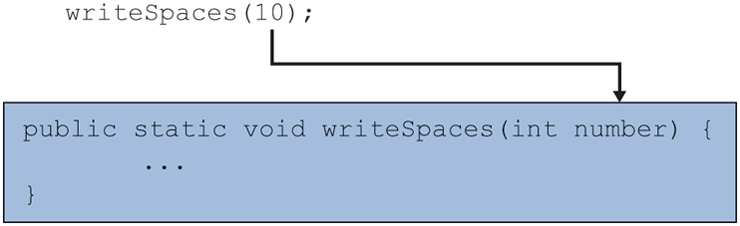
\includegraphics[width=\maxwidth,height=\maxheight,keepaspectratio,alt={Image}]{Figures/img_p6_0.png}}
\end{center}


\caption{Image}
\end{figure}

Tham số \texttt{number} là một biến cục bộ, nhưng nó nhận giá trị ban
đầu từ lời gọi. Gọi phương thức này với giá trị \texttt{10} tương đương
với việc bao gồm khai báo sau ở phần đầu của phương thức
\texttt{writeSpaces}:

\begin{verbatim}
int number = 10;
\end{verbatim}

Tất nhiên, cơ chế này linh hoạt hơn so với một khai báo biến cụ thể, bởi
vì thay vào đó, bạn có thể viết:

\begin{verbatim}
writeSpaces(20);
\end{verbatim}

và nó sẽ giống như thể bạn đã viết:

\begin{verbatim}
int number = 20;
\end{verbatim}

ở phần đầu của phương thức. Thậm chí bạn có thể sử dụng một biểu thức số
nguyên cho lời gọi:

\begin{verbatim}
writeSpaces(3 * 4 - 5);
\end{verbatim}

Trong trường hợp này, Java tính toán biểu thức để nhận được giá trị
\texttt{7} và sau đó gọi \texttt{writeSpaces}, khởi tạo \texttt{number}
bằng \texttt{7}.

Các nhà khoa học máy tính sử dụng từ ``tham số'' (parameter) theo nghĩa
rộng để chỉ cả những gì xuất hiện trong phần tiêu đề phương thức (tham
số hình thức) và những gì xuất hiện trong lời gọi phương thức (tham số
thực tế).

\textbf{Tham số Hình thức (Formal Parameter)} \textgreater{} Một biến
xuất hiện bên trong dấu ngoặc đơn ở phần tiêu đề của một phương thức,
được sử dụng để khái quát hóa (generalize) hành vi của phương thức đó.

\textbf{Tham số Thực tế (Actual Parameter)} \textgreater{} Một giá trị
hoặc một biểu thức cụ thể xuất hiện bên trong dấu ngoặc đơn trong một
lời gọi phương thức.

Thuật ngữ ``tham số hình thức'' không mô tả mục đích của nó. Một cái tên
tốt hơn sẽ là ``tham số khái quát'' (generalized parameter). Trong
phương thức \texttt{writeSpaces}, \texttt{number} là tham số khái quát
xuất hiện trong khai báo phương thức. Nó là một chỗ giữ (placeholder)
cho một số giá trị chưa được chỉ định. Các giá trị xuất hiện trong các
lời gọi phương thức là các tham số thực tế, bởi vì mỗi lời gọi chỉ ra
một tác vụ cụ thể cần thực hiện. Nói cách khác, mỗi lời gọi cung cấp một
giá trị thực tế để điền vào chỗ giữ.

Từ ``đối số'' (argument) thường được sử dụng như một từ đồng nghĩa với
``tham số'', chẳng hạn như trong câu ``Đây là những đối số (arguments)
tôi đang truyền cho phương thức này''. Một số người thích dành từ ``đối
số'' (argument) cho các tham số thực tế và từ ``tham số'' (parameter)
cho các tham số hình thức.

Hãy xem xét một ví dụ về cách bạn có thể sử dụng phương thức
\texttt{writeSpaces} này. Hãy nhớ rằng chương trình \texttt{DrawFigure2}
có phương thức sau đây, được gọi là \texttt{drawTop}:

\begin{verbatim}
// produces the top half of the hourglass figure
public static void drawTop() {
    for (int line = 1; line <= SUB_HEIGHT; line++) {
        System.out.print("|");
        for (int i = 1; i <= (line - 1); i++) {
            System.out.print(" ");
        }
        System.out.print("\\");
        int dots = 2 * SUB_HEIGHT - 2 * line;
        for (int i = 1; i <= dots; i++) {
            System.out.print(".");
        }
        System.out.print("/");
        for (int i = 1; i <= (line - 1); i++) {
            System.out.print(" ");
        }
        System.out.println("|");
    }
}
\end{verbatim}

Bằng cách sử dụng phương thức \texttt{writeSpaces}, bạn có thể viết lại
phương thức này như sau:

\begin{verbatim}
public static void drawTop() {
    for (int line = 1; line <= SUB_HEIGHT; line++) {
        System.out.print("|");
        writeSpaces(line - 1);
\end{verbatim}

\begin{verbatim}
    System.out.println("|");
}
\end{verbatim}

\}

\begin{verbatim}

Lưu ý rằng `writeSpaces` được gọi ở hai thời điểm khác nhau, chỉ định số lượng khoảng trắng cần thiết trong mỗi trường hợp. Bạn có thể sửa đổi phương thức `drawBottom` từ chương trình `DrawFigure2` theo cách tương tự để đơn giản hóa nó.

Bạn có thể viết toàn bộ một phương thức trong JShell để kiểm tra các tham số. Dưới đây là một phương thức có tên `writeStars` để in một số lượng dấu hoa thị nhất định ra giao diện điều khiển (console):
```java
jshell> public static void writeStars(int number) {
   ...>     for (int i = 1; i <= number; i++) {
   ...>         System.out.print("*");
   ...>     }
   ...> }
|  created method writeStars(int)
\end{verbatim}

\begin{verbatim}
jshell> writeStars(5);
*****
jshell> writeStars(8);
********
\end{verbatim}

\subsubsection{Cơ chế của các Tham số (The Mechanics of
Parameters)}\label{cux1a1-chux1ebf-cux1ee7a-cuxe1c-tham-sux1ed1-the-mechanics-of-parameters}

Khi Java thực thi một lời gọi đến một phương thức, nó sẽ khởi tạo các
tham số của phương thức đó. Đối với mỗi tham số, đầu tiên nó sẽ tính
toán biểu thức được truyền vào dưới dạng tham số thực tế (actual
parameter) và sau đó sử dụng kết quả đó để khởi tạo biến cục bộ có tên
được cung cấp bởi tham số hình thức (formal parameter).

Hãy sử dụng một ví dụ để làm rõ quá trình này:

\begin{verbatim}
 1  // Demonstrates parameters with a method for writing spaces.
 2  public class ParameterExample {
 3      public static void main(String[] args) {
\end{verbatim}

\begin{verbatim}
 4          int spaces1 = 3;
 5          int spaces2 = 5;
 6
 7          System.out.print("*");
 8          writeSpaces(spaces1);
 9          System.out.println("*");
 10
 11          System.out.print("!");
 12          writeSpaces(spaces2);
 13          System.out.println("!");
 14
 15          System.out.print("'");
 16          writeSpaces(8);
 17          System.out.println("'");
 18
 19          System.out.print("<");
 20          writeSpaces(spaces1 * spaces2 - 5);
 21          System.out.println(">");
 22      }
 23
 24      // writes "number" spaces on the current output line
 25      public static void writeSpaces(int number) {
 26          for (int i = 1; i <= number; i++) {
 27              System.out.print(" ");
 28          }
 29      }
 30  }
\end{verbatim}

Trong hai dòng đầu tiên của phương thức \texttt{main}, máy tính tìm thấy
các lệnh để cấp phát và khởi tạo hai biến:

Ba dòng mã tiếp theo tạo ra một dòng kết quả đầu ra với ba khoảng trắng
được bao quanh bởi các dấu hoa thị ở hai bên:

\begin{verbatim}
System.out.print("*");
writeSpaces(spaces1);
System.out.println("*");
\end{verbatim}

Bạn có thể thấy các dấu hoa thị đến từ đâu, nhưng hãy nhìn vào lời gọi
phương thức tạo ra các khoảng trắng. Khi Java thực thi lời gọi tới
\texttt{writeSpaces}, nó phải thiết lập tham số của nó. Để thiết lập
tham số, đầu tiên Java tính toán biểu thức được truyền vào dưới dạng
tham số thực tế. Biểu thức này đơn giản là biến \texttt{spaces1}, biến
có giá trị là \texttt{3}. Do đó, biểu thức được tính toán ra \texttt{3}.
Java sử dụng kết quả này để khởi tạo một biến cục bộ có tên là
\texttt{number}.

Sơ đồ dưới đây chỉ ra cách bộ nhớ của máy tính sẽ trông như thế nào khi
phương thức \texttt{writeSpaces} được tiến vào lần đầu tiên. Bởi vì có
hai phương thức liên quan (là \texttt{main} và \texttt{writeSpaces}), sơ
đồ sẽ chỉ ra những biến nào là cục bộ đối với \texttt{main}
(\texttt{spaces1} và \texttt{spaces2}) và những biến nào là cục bộ đối
với \texttt{writeSpaces} (tham số \texttt{number}):

\begin{figure}
\centering


\begin{center}
\pandocbounded{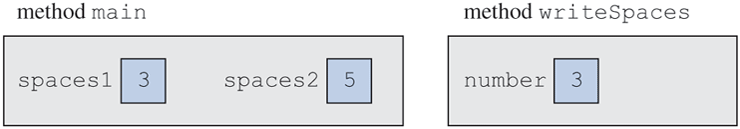
\includegraphics[width=\maxwidth,height=\maxheight,keepaspectratio,alt={Image}]{Figures/img_p14_0.png}}
\end{center}


\caption{Image}
\end{figure}

Tác dụng thực tế của quá trình này là phương thức \texttt{writeSpaces}
có một bản sao cục bộ của giá trị được lưu trong biến \texttt{spaces1}
từ phương thức \texttt{main}. Câu lệnh \texttt{println} xuất hiện sau
lời gọi tới \texttt{writeSpaces} sẽ đặt một dấu hoa thị vào cuối dòng và
sau đó hoàn thành dòng kết quả đầu ra.

Bây giờ hãy theo dõi ba dòng mã tiếp theo:

\begin{verbatim}
System.out.print("!");
writeSpaces(spaces2);
System.out.println("!");
\end{verbatim}

Dòng đầu tiên in ra một dấu chấm than trên dòng kết quả đầu ra thứ hai,
sau đó gọi \texttt{writeSpaces} một lần nữa, lần này với biến
\texttt{spaces2} là tham số thực tế của nó. Máy tính tính toán biểu thức
này, thu được kết quả \texttt{5}. Giá trị này được sử dụng để khởi tạo
\texttt{number}. Như vậy,

lần này nó tạo ra một bản sao của giá trị được lưu trong biến
\texttt{spaces2} từ phương thức \texttt{main}:

\begin{figure}
\centering


\begin{center}
\pandocbounded{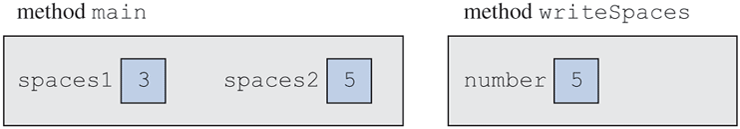
\includegraphics[width=\maxwidth,height=\maxheight,keepaspectratio,alt={Image}]{Figures/img_p15_0.png}}
\end{center}


\caption{Image}
\end{figure}

Vì lần này \texttt{number} có một giá trị khác (\texttt{5} thay vì
\texttt{3}), phương thức tạo ra một số lượng khoảng trắng khác. Sau khi
phương thức thực thi, \texttt{println} kết thúc dòng kết quả đầu ra bằng
một dấu chấm than thứ hai.

Dưới đây là ba dòng mã tiếp theo:

\begin{verbatim}
System.out.print("'");
writeSpaces(8);
System.out.println("'");
\end{verbatim}

Đoạn mã này in ra một dấu nháy đơn ở đầu dòng kết quả đầu ra thứ ba và
sau đó gọi lại \texttt{writeSpaces}. Lần này nó sử dụng hằng số nguyên
\texttt{8} làm biểu thức, điều đó có nghĩa là nó khởi tạo tham số
\texttt{number} như một bản sao của số \texttt{8}:

\begin{figure}
\centering


\begin{center}
\pandocbounded{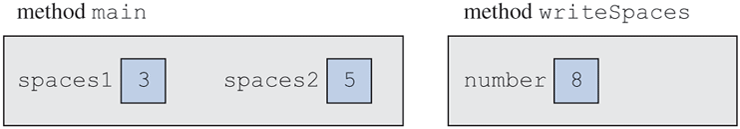
\includegraphics[width=\maxwidth,height=\maxheight,keepaspectratio,alt={Image}]{Figures/img_p16_0.png}}
\end{center}


\caption{Image}
\end{figure}

Một lần nữa, phương thức sẽ hoạt động khác đi do giá trị khác nhau của
\texttt{number}. Nó in ra tám khoảng trắng trên dòng và kết thúc thực
thi. Sau đó \texttt{println} hoàn thành dòng kết quả đầu ra bằng cách in
một dấu nháy đơn khác ở cuối dòng.

Cuối cùng, ba dòng mã cuối cùng trong phương thức \texttt{main} là:

\begin{verbatim}
System.out.print("<");
writeSpaces(spaces1 * spaces2 - 5);
System.out.println(">");
\end{verbatim}

Đoạn mã này in ra một ký tự nhỏ hơn (\texttt{\textless{}}) ở đầu dòng
kết quả đầu ra thứ tư và sau đó thực hiện lời gọi cuối cùng tới phương
thức \texttt{writeSpaces}. Lần này tham số thực tế là một biểu thức,
không chỉ là một biến hay một giá trị hằng. Do đó, trước khi lời gọi
được thực hiện, máy tính sẽ tính toán biểu thức để xác định giá trị của
nó:

\begin{figure}
\centering


\begin{center}
\pandocbounded{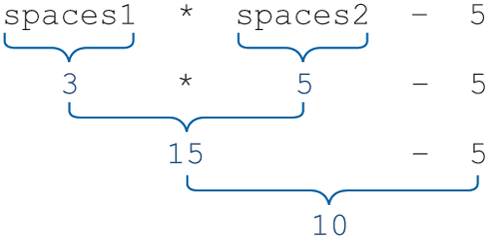
\includegraphics[width=\maxwidth,height=\maxheight,keepaspectratio,alt={Image}]{Figures/img_p17_0.png}}
\end{center}


\caption{Image}
\end{figure}

Máy tính sử dụng kết quả này để khởi tạo \texttt{number}:

\begin{figure}
\centering


\begin{center}
\pandocbounded{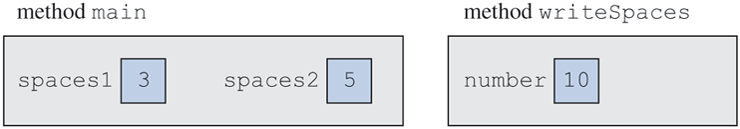
\includegraphics[width=\maxwidth,height=\maxheight,keepaspectratio,alt={Image}]{Figures/img_p17_1.png}}
\end{center}


\caption{Image}
\end{figure}

Bây giờ \texttt{number} là một bản sao của giá trị được mô tả bởi biểu
thức phức tạp này. Vì vậy, tổng kết quả đầu ra của chương trình này là:

\begin{verbatim}
*   * 
!     ! 
'       ' 
<         >
\end{verbatim}

\begin{quote}
\textbf{LỖI LẬP TRÌNH PHỔ BIẾN (COMMON PROGRAMMING ERROR)}

\textbf{Nhầm lẫn giữa các Tham số Thực tế và Hình thức (Confusing Actual
and Formal Parameters)}

Nhiều sinh viên đã quen với việc nhìn thấy các khai báo của các tham số
hình thức và lầm tưởng rằng cú pháp của chúng giống hệt với cú pháp
truyền các tham số thực tế. Một sai lầm phổ biến là viết cả kiểu của một
biến khi nó đang được truyền vào như một tham số:

\begin{verbatim}
writeSpaces(int spaces1); // this doesn’t work
\end{verbatim}

Sự nhầm lẫn này là do kiểu của tham số được viết trong phần khai báo của
phương thức, giống như thế này:

\begin{verbatim}
public static void writeSpaces(int number)
\end{verbatim}

Các kiểu (types) phải được viết ra khi các biến hoặc các tham số được
khai báo, nhưng khi các biến được sử dụng, chẳng hạn như khi mã gọi một
phương thức và truyền các biến vào dưới dạng các tham số thực tế, thì
kiểu của chúng sẽ không được viết. Các tham số thực tế không phải là các
khai báo; do đó, các kiểu không nên được viết trước chúng:

\begin{verbatim}
writeSpaces(spaces1); // much better!
\end{verbatim}
\end{quote}

\subsubsection{Những hạn chế của Tham số (Limitations of
Parameters)}\label{nhux1eefng-hux1ea1n-chux1ebf-cux1ee7a-tham-sux1ed1-limitations-of-parameters}

Chúng ta đã thấy rằng một tham số có thể được sử dụng để cung cấp đầu
vào cho một phương thức. Nhưng trong khi bạn có thể sử dụng một tham số
để gửi một giá trị vào một phương thức, bạn không thể sử dụng một tham
số để lấy một giá trị ra khỏi một phương thức. Khi một tham số được
thiết lập, một biến cục bộ được tạo ra và được khởi tạo bằng giá trị
được truyền vào dưới dạng tham số thực tế. Tác dụng thực tế là biến cục
bộ đó là một bản sao của giá trị đến từ bên ngoài. Vì nó là một biến cục
bộ, nó không thể ảnh hưởng đến bất kỳ biến nào bên ngoài phương thức.
Hãy xem xét chương trình mẫu sau:

\begin{verbatim}
 1  // A demonstration of parameter limitations.
 2  public class ParameterExample2 {
 3      public static void main(String[] args) {
 4          int x = 17;
 5          doubleNumber(x);
 6          System.out.println("x = " + x);
 7          System.out.println();
 8
 9          int number = 42;
\end{verbatim}

10 doubleNumber(number); 11 System.out.println(``number ='' + number);
12 \} 13 14 public static void doubleNumber(int number) \{ 15
System.out.println(``Initial value ='' + number); 16 number = number *
2; 17 System.out.println(``Final value ='' + number); 18 \} 19 \}

\begin{verbatim}

Chương trình này bắt đầu bằng việc khai báo và khởi tạo một biến số nguyên được gọi là `x` với giá trị `17`:



Sau đó, nó gọi phương thức `doubleNumber`, truyền `x` vào dưới dạng một tham số. Giá trị của `x` được sử dụng để khởi tạo tham số `number` như một biến cục bộ của phương thức có tên `doubleNumber`:

![Image](Figures/img_p21_0.png)

Tiếp theo, chương trình thực thi các câu lệnh bên trong `doubleNumber`. Đầu tiên, `doubleNumber` in ra giá trị ban đầu của `number` (`17`). Sau đó, nó nhân đôi `number`:

![Image](Figures/img_p21_1.png)

Lưu ý rằng điều này không có tác động gì đến biến `x`. Tham số được gọi là `number` là một bản sao của `x`, vì vậy mặc dù chúng bắt đầu giống nhau, việc thay đổi giá trị của `number` không làm ảnh hưởng đến `x`. Tiếp đó, `doubleNumber` báo cáo giá trị mới của `number` (`34`).

Tại thời điểm này, `doubleNumber` kết thúc thực thi và chúng ta trở về `main`:



Câu lệnh tiếp theo trong phương thức `main` báo cáo giá trị của `x`, đó là `17`. Sau đó, nó khai báo và khởi tạo một biến được gọi là `number` với giá trị `42`:



Câu lệnh sau đó gọi `doubleNumber` một lần nữa, lần này truyền cho nó giá trị của `number`. Đây là một tình huống kỳ lạ vì tham số này có cùng tên với biến trong `main`, nhưng Java không quan tâm. Nó luôn tạo ra một biến cục bộ mới cho phương thức `doubleNumber`:



Vì vậy, tại thời điểm này có hai biến khác nhau được gọi là `number`, mỗi biến ở một phương thức. Bây giờ là lúc để thực thi các câu lệnh của `doubleNumber` một lần nữa. Đầu tiên nó báo cáo giá trị của `number` (`42`), sau đó nhân đôi nó:



Một lần nữa, lưu ý rằng việc nhân đôi `number` bên trong `doubleNumber` không có tác động gì đến biến ban đầu `number` trong `main`. Đây là các biến riêng biệt. Phương thức sau đó báo cáo giá trị mới của `number` (`84`) và trở về `main`:



Tiếp đó, chương trình báo cáo giá trị của `number` và kết thúc. Vì vậy, tổng thể kết quả đầu ra của chương trình như sau:
```text
Initial value = 17 
Final value = 34 
x = 17 
 
Initial value = 42 
Final value = 84 
number = 42
\end{verbatim}

Các thao tác cục bộ đối với tham số không làm thay đổi những biến này ở
bên ngoài phương thức. Việc các biến được sao chép là một khía cạnh quan
trọng của các tham số. Về mặt tích cực, chúng ta biết rằng các biến được
bảo vệ khỏi sự thay đổi vì các tham số là những bản sao của biến gốc. Về
mặt tiêu cực, điều này có nghĩa là mặc dù các tham số sẽ cho phép chúng
ta gửi các giá trị vào một phương thức, chúng sẽ không cho phép chúng ta
lấy các giá trị trở lại ra khỏi một phương thức.

\subsubsection{Nhiều Tham số (Multiple
Parameters)}\label{nhiux1ec1u-tham-sux1ed1-multiple-parameters}

Cho đến nay, cuộc thảo luận của chúng ta về cú pháp của tham số vẫn mang
tính không chính thức. Đã đến lúc chúng ta viết ra một cách chính xác
hơn cú pháp chúng ta sử dụng để khai báo các phương thức tĩnh có chứa
tham số. Dưới đây là cú pháp đó:

\begin{verbatim}
public static void <name>(<type> <name>, ..., <type> <name>) {
    <statement>;
    <statement>;
    ...
\end{verbatim}

\begin{verbatim}
    <statement>;
}
\end{verbatim}

Bản mẫu (template) này chỉ ra rằng chúng ta có thể khai báo bao nhiêu
tham số tùy thích bên trong cặp ngoặc đơn xuất hiện sau tên của một
phương thức trong tiêu đề của nó. Chúng ta sử dụng dấu phẩy để phân tách
các tham số khác nhau.

Lấy ví dụ về một phương thức có nhiều tham số, hãy xem xét một biến thể
của \texttt{writeSpaces}. Thật tiện lợi khi chúng ta có thể sử dụng
phương thức này để in ra số lượng khoảng trắng khác nhau, nhưng nó luôn
chỉ in khoảng trắng. Điều gì sẽ xảy ra nếu chúng ta muốn 18 dấu hoa thị,
hoặc 23 dấu chấm, hay 17 dấu chấm hỏi? Chúng ta có thể khái quát hóa tác
vụ này xa hơn nữa bằng cách cho phương thức nhận hai tham số---một ký tự
và số lần in ký tự đó:

\begin{verbatim}
public static void writeChars(char ch, int number) {
    for (int i = 1; i <= number; i++) {
        System.out.print(ch);
    }
}
\end{verbatim}

Ký tự cần in ra là một tham số có kiểu \texttt{char}, chúng ta sẽ thảo
luận chi tiết hơn về kiểu này trong chương tiếp theo. Hãy nhớ lại rằng
các hằng ký tự (character literals) được đặt trong các dấu nháy đơn.

Bản mẫu cú pháp để gọi một phương thức nhận tham số là như sau:

\begin{verbatim}
<method name>(<expression>, <expression>, ..., <expression>);
\end{verbatim}

Bằng cách gọi phương thức \texttt{writeChars}, bạn có thể viết mã giống
như sau:

\begin{verbatim}
writeChars('=', 20);
System.out.println();
for (int i = 1; i <= 10; i++) {
    writeChars('>', i);
    writeChars(' ', 20 - 2 * i);
    writeChars('<', i);
    System.out.println();
}
\end{verbatim}

Đoạn mã này tạo ra kết quả đầu ra sau:

\begin{verbatim}
==================== 
>                  < 
>>                << 
>>>              <<< 
>>>>            <<<< 
>>>>>          <<<<< 
>>>>>>        <<<<<< 
>>>>>>>      <<<<<<< 
>>>>>>>>    <<<<<<<< 
>>>>>>>>>  <<<<<<<<< 
>>>>>>>>>><<<<<<<<<<
\end{verbatim}

Bằng cách sử dụng phương thức \texttt{writeChars}, chúng ta có thể viết
một phiên bản thậm chí còn tốt hơn của phương thức \texttt{drawTop} từ
chương trình \texttt{DrawFigure2} ở Chương 2.

Chúng ta đã thấy trước đó rằng bằng cách sử dụng \texttt{writeSpaces},
chúng ta có thể loại bỏ hai trong số các vòng lặp bên trong, nhưng điều
này vẫn để lại cho chúng ta vòng lặp bên trong để in các dấu chấm. Bây
giờ, chúng ta có thể loại bỏ tất cả ba vòng lặp bên trong và tạo ra một
phiên bản dễ đọc hơn nhiều của phương thức này:

\begin{verbatim}
public static void drawTop() {
    for (int line = 1; line <= SUB_HEIGHT; line++) {
        System.out.print("|");
        writeChars(' ', line - 1);
        System.out.print("\\");
        writeChars('.', 2 * SUB_HEIGHT - 2 * line);
        System.out.print("/");
        writeChars(' ', line - 1);
        System.out.println("|");
    }
}
\end{verbatim}

Bạn có thể bao gồm bao nhiêu tham số tùy thích khi bạn định nghĩa một
phương thức. Mỗi lời gọi phương thức phải cung cấp chính xác số lượng
tham số đó, theo cùng một thứ tự. Ví dụ, hãy xem xét lời gọi đầu tiên
tới \texttt{writeChars} trong đoạn mã trước đó và tiêu đề của
\texttt{writeChars}. Java xếp hàng các tham số theo thứ tự tuần tự (với
tham số thực tế đầu tiên đi vào tham số hình thức đầu tiên và tham số
thực tế thứ hai đi vào tham số hình thức thứ hai):

\begin{figure}
\centering


\begin{center}
\pandocbounded{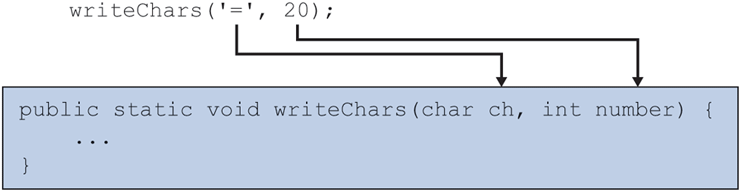
\includegraphics[width=\maxwidth,height=\maxheight,keepaspectratio,alt={Image}]{Figures/img_p28_0.png}}
\end{center}


\caption{Image}
\end{figure}

Chúng ta đã thấy rằng các phương thức có thể gọi các phương thức khác;
điều này cũng đúng với các phương thức nhận tham số. Ví dụ, đây là một
phương thức dùng để vẽ một hộp có chiều cao và chiều rộng nhất định có
gọi đến phương thức \texttt{writeChars}:

\begin{verbatim}
public static void drawBox(int height, int width) {
    // draw top of box
    writeChars('*', width);
    System.out.println();

    // draw middle lines
    for (int i = 1; i <= height - 2; i++) {
        System.out.print('*');
        writeChars(' ', width - 2);
        System.out.println("*");
    }
    // draw bottom of box
    writeChars('*', width);
    System.out.println();
}
\end{verbatim}

Lưu ý rằng \texttt{drawBox} được truyền các giá trị cho các tham số có
tên là \texttt{height} và \texttt{width}, và các tham số này được sử
dụng để tạo thành các biểu thức được truyền dưới dạng giá trị cho
\texttt{writeChars}. Ví dụ, bên trong vòng lặp \texttt{for}, chúng ta
gọi \texttt{writeChars} yêu cầu nó tạo ra \texttt{width\ -\ 2} khoảng
trắng. (Chúng ta trừ đi 2 vì chúng ta in một dấu sao ở đầu và ở cuối
dòng.) Dưới đây là một lời gọi mẫu tới phương thức này:

\begin{verbatim}
drawBox(5, 10);
\end{verbatim}

Đoạn mã này tạo ra kết quả đầu ra sau:

\begin{center}\rule{0.5\linewidth}{0.5pt}\end{center}

\begin{itemize}
\item
\begin{verbatim}
   * 
\end{verbatim}
\item
\begin{verbatim}
   * 
\end{verbatim}
\item
\begin{verbatim}
   * 
\end{verbatim}

  \begin{center}\rule{0.5\linewidth}{0.5pt}\end{center}
\end{itemize}

\begin{verbatim}

Khi bạn viết các phương thức nhận nhiều tham số, phần tiêu đề phương thức có thể trở nên rất dài. Người ta thường ngắt các dòng dài (những dòng vượt quá khoảng 80 ký tự) bằng cách chèn một ngắt dòng sau một toán tử hoặc một tham số và thụt lề dòng tiếp theo bằng hai lần độ rộng thụt lề thông thường:
```java
// this method’s header is too long, so we’ll wrap it
public static void printTriangle(int xCoord1, int yCoord1,
        int xCoord2, int yCoord2, int xCoord3, int yCoord3) {
  ...
}
\end{verbatim}

\subsubsection{Tham số so với Hằng số (Parameters versus
Constants)}\label{tham-sux1ed1-so-vux1edbi-hux1eb1ng-sux1ed1-parameters-versus-constants}

Trong Chương 2, bạn đã thấy rằng các hằng số của lớp là một cơ chế hữu
ích để tăng tính linh hoạt cho các chương trình của bạn. Bằng cách sử
dụng các hằng số như vậy, bạn có thể dễ dàng sửa đổi một chương trình để
nó hoạt động khác đi. Các tham số cung cấp nhiều sự linh hoạt tương tự,
và còn nhiều hơn thế. Hãy xem xét phương thức \texttt{writeSpaces}. Giả
sử bạn viết nó bằng cách sử dụng một hằng số của lớp:

\begin{verbatim}
public static final int NUMBER_OF_SPACES = 10;
\end{verbatim}

Cách tiếp cận này sẽ mang lại cho bạn sự linh hoạt để tạo ra một số
lượng khoảng trắng khác nhau, nhưng nó có một hạn chế lớn: Hằng số chỉ
có thể thay đổi từ lần thực thi này sang lần thực thi khác; nó không thể
thay đổi trong một lần thực thi duy nhất. Nói cách khác, bạn có thể thực
thi chương trình một lần với một giá trị, chỉnh sửa chương trình, biên
dịch lại, và sau đó thực thi lại với một giá trị khác, nhưng bạn không
thể sử dụng các giá trị khác nhau trong một lần thực thi chương trình
nếu sử dụng một hằng số của lớp.

Các tham số thì linh hoạt hơn. Bởi vì bạn chỉ định giá trị sẽ được sử
dụng mỗi khi bạn gọi phương thức, bạn có thể sử dụng một vài giá trị
khác nhau trong một lần thực thi chương trình. Như bạn đã thấy, bạn có
thể gọi phương thức nhiều lần khác nhau trong một lần thực thi chương
trình và làm cho nó hoạt động khác nhau ở mỗi lần. Tuy nhiên, việc sử
dụng các tham số đòi hỏi lập trình viên phải làm nhiều việc hơn so với
việc sử dụng các hằng số của lớp. Nó làm cho các tiêu đề phương thức và
các lời gọi phương thức trở nên tẻ nhạt hơn, chưa kể đến việc làm cho
quá trình thực thi (và do đó, quá trình gỡ lỗi) trở nên phức tạp hơn.

Vì vậy, có thể bạn sẽ tìm thấy dịp để sử dụng mỗi kỹ thuật. Quy tắc cơ
bản là hãy sử dụng một hằng số của lớp khi bạn chỉ muốn thay đổi giá trị
từ lần thực thi này sang lần thực thi khác. Nếu bạn muốn sử dụng các giá
trị khác nhau trong một lần thực thi duy nhất, hãy sử dụng một tham số.

\subsubsection{Nạp chồng Phương thức (Overloading of
Methods)}\label{nux1ea1p-chux1ed3ng-phux1b0ux1a1ng-thux1ee9c-overloading-of-methods}

Bạn sẽ thường muốn tạo ra những biến thể nhỏ của cùng một phương thức
bằng cách truyền vào các tham số khác nhau. Ví dụ, bạn có thể có một
phương thức \texttt{drawBox} cho phép bạn chỉ định một chiều cao và
chiều rộng cụ thể, nhưng bạn cũng có thể muốn có một phiên bản vẽ một
cái hộp với kích thước mặc định. Nói cách khác, đôi khi bạn muốn chỉ
định các giá trị này, như trong:

\begin{verbatim}
drawBox(8, 10);
\end{verbatim}

và những lần khác bạn chỉ muốn vẽ một cái hộp với chiều cao và chiều
rộng tiêu chuẩn:

\begin{verbatim}
drawBox();
\end{verbatim}

Một số ngôn ngữ lập trình yêu cầu bạn phải nghĩ ra các tên khác nhau cho
những phiên bản này, chẳng hạn như \texttt{drawBox} và
\texttt{drawDefaultBox}. Như bạn có thể tưởng tượng, việc nghĩ ra tên
mới cho mỗi biến thể trở nên tẻ nhạt. Thật may mắn, Java cho phép bạn có
nhiều hơn một phương thức có cùng tên, miễn là chúng có các tham số khác
nhau. Điều này được gọi là nạp chồng (overloading). Yêu cầu chính đối
với việc nạp chồng là các phương thức khác nhau mà bạn định nghĩa phải
có các chữ ký phương thức (method signatures) khác nhau.

\begin{quote}
\textbf{Nạp chồng Phương thức (Method Overloading)}

Khả năng định nghĩa hai hoặc nhiều phương thức khác nhau có cùng tên
nhưng khác chữ ký phương thức.

\textbf{Chữ ký Phương thức (Method Signature)}

Tên của một phương thức, cùng với số lượng và kiểu của các tham số của
nó.
\end{quote}

Hai phiên bản \texttt{drawBox} trong ví dụ rõ ràng có các chữ ký phương
thức khác nhau, bởi vì một phương thức có hai tham số và phương thức kia
có không tham số. Từ bất kỳ lời gọi nào tới phương thức cũng sẽ rõ ràng
về việc sử dụng phiên bản nào: Nếu bạn thấy có hai tham số, bạn thực thi
phiên bản có hai tham số; nếu bạn thấy không có tham số nào, bạn thực
thi phiên bản có không tham số.

Tình huống trở nên phức tạp hơn khi việc nạp chồng liên quan đến cùng
một số lượng tham số, nhưng điều này hóa ra lại là một trong những ứng
dụng hữu ích nhất của việc nạp chồng. Ví dụ, phương thức
\texttt{println} thực tế là một chuỗi các phương thức được nạp chồng.
Chúng ta có thể gọi \texttt{println} bằng cách truyền cho nó một
\texttt{String}, một \texttt{int}, một \texttt{double}, v.v. Sự linh
hoạt này được triển khai dưới dạng một loạt các phương thức khác nhau,
tất cả đều nhận một tham số: Một phiên bản nhận một \texttt{String}, một
phiên bản khác nhận một \texttt{int}, một phiên bản khác nữa nhận một
\texttt{double}, và cứ tiếp tục như vậy. Rõ ràng là bạn thực hiện các
thao tác hơi khác nhau để in ra một trong những loại dữ liệu này so với
các loại dữ liệu khác, đó là lý do tại sao việc có các phiên bản khác
nhau của phương thức là rất hữu ích.

\subsection{Các Phương thức Trả về Giá trị (Methods That Return
Values)}\label{cuxe1c-phux1b0ux1a1ng-thux1ee9c-trux1ea3-vux1ec1-giuxe1-trux1ecb-methods-that-return-values-1}

Vài phương thức cuối cùng mà chúng ta đã xem xét là các phương thức định
hướng hành động (action-oriented) nhằm thực hiện một số tác vụ cụ thể.
Bạn có thể coi chúng giống như các mệnh lệnh mà bạn có thể ra lệnh cho
ai đó, như ``Hãy vẽ một hộp'' hoặc ``Hãy vẽ một hình tam giác.'' Các
tham số cho phép các mệnh lệnh này trở nên linh hoạt hơn, như ``Hãy vẽ
một hộp có kích thước 10 x 20.''

Bạn cũng sẽ muốn có thể viết các phương thức dùng để tính toán các giá
trị. Những phương thức này giống như các câu hỏi hơn, như ``Căn bậc hai
của 2.5 là bao nhiêu?'' hoặc ``Bạn nhận được gì khi lũy thừa bậc 4 của
2.3?'' Lấy ví dụ, hãy xem xét một phương thức tên là \texttt{sqrt} sẽ
tính căn bậc hai của một số.

Có vẻ như cách để viết một phương thức như vậy sẽ là để nó nhận một tham
số kiểu \texttt{double} và in ra (bằng \texttt{println}) căn bậc hai của
nó ra giao diện điều khiển (console). Nhưng bạn có thể muốn sử dụng căn
bậc hai như một phần của một biểu thức hoặc một phép tính lớn hơn, chẳng
hạn như giải một phương trình bậc hai hoặc tính toán khoảng cách giữa
các điểm trên một mặt phẳng tọa độ \(x/y\).

Một giải pháp tốt hơn sẽ là một lệnh căn bậc hai (square root command)
truyền con số đang được quan tâm vào dưới dạng một tham số và trả về
(return) căn bậc hai của nó cho chương trình như một kết quả. Sau đó,
bạn có thể sử dụng kết quả đó như một phần của một biểu thức, lưu nó vào
một biến, hoặc in nó ra giao diện điều khiển. Một lệnh như vậy là một
kiểu phương thức mới được cho là sẽ trả về một giá trị.

\begin{quote}
\textbf{Trả về (Return)}

Việc gửi một giá trị ra ngoài dưới dạng kết quả của một phương thức có
thể được sử dụng trong một biểu thức trong chương trình của bạn. Các
phương thức void không trả về bất kỳ giá trị nào.
\end{quote}

Nếu bạn có một phương thức như vậy, bạn có thể yêu cầu lấy căn bậc hai
của 2.5 bằng cách viết đoạn mã như thế này:

\begin{verbatim}
// assuming you had a method called sqrt
double answer = sqrt(2.5);
\end{verbatim}

Phương thức \texttt{sqrt} có một tham số (số mà bạn muốn tìm căn bậc
hai), và nó cũng trả về một giá trị (căn bậc hai đó). Tham số thực tế
\texttt{2.5} đi ``vào trong'' phương thức, và căn bậc hai đi ra. Trong
đoạn mã trước, kết quả được trả về sẽ được lưu trong một biến có tên là
\texttt{answer}.

Bạn có thể biết được liệu một phương thức có trả về một giá trị hay
không bằng cách nhìn vào tiêu đề của nó. Tất cả các phương thức bạn đã
viết cho đến nay đều bắt đầu bằng \texttt{public\ static\ void}. Từ
\texttt{void} được gọi là kiểu trả về (return type) của phương thức.

Kiểu trả về \texttt{void} hơi kỳ lạ một chút bởi vì, đúng như tên gọi
của nó, phương thức không trả về gì cả. Một phương thức có thể trả về
bất kỳ kiểu hợp lệ nào: một \texttt{int}, một \texttt{double}, hoặc bất
kỳ kiểu nào khác. Trong trường hợp của phương thức \texttt{sqrt}, bạn
muốn nó trả về một \texttt{double}, vì vậy bạn sẽ viết tiêu đề của nó
như sau:

\begin{verbatim}
public static double sqrt(double n)
\end{verbatim}

Giống như trường hợp trước, từ đứng sau \texttt{public\ static} là kiểu
trả về của phương thức:

May mắn thay, bạn không thực sự cần phải viết một phương thức để tính
căn bậc hai của một số, bởi vì Java đã có sẵn một phương thức được tích
hợp (built in). Phương thức này được bao gồm trong một lớp có tên là
\texttt{Math}, lớp này bao gồm nhiều phương thức tính toán hữu ích. Vì
vậy, trước khi chúng ta thảo luận chi tiết về việc viết các phương thức
trả về các giá trị, hãy cùng khám phá lớp \texttt{Math} và xem nó cung
cấp những gì.

\subsubsection{Lớp Math (The Math
Class)}\label{lux1edbp-math-the-math-class}

Trong Chương 1, chúng ta đã đề cập rằng rất nhiều mã định nghĩa sẵn,
được gọi chung là các thư viện lớp Java (Java class libraries), đã được
viết cho Java. Một trong những lớp hữu ích nhất là \texttt{Math}. Nó bao
gồm các hằng số toán học được định nghĩa sẵn và một số lượng lớn các hàm
toán học thông dụng. Lớp \texttt{Math} sẽ có sẵn trên bất kỳ máy nào
được cài đặt Java đúng cách.

Như chúng ta đã lưu ý trong phần trước, lớp \texttt{Math} có một phương
thức tên là \texttt{sqrt} dùng để tính căn bậc hai của một số. Phương
thức này có tiêu đề như sau:

\begin{verbatim}
public static double sqrt(double n)
\end{verbatim}

Tiêu đề này nói rằng phương thức có tên là \texttt{sqrt}, nó nhận một
tham số kiểu \texttt{double}, và nó trả về một giá trị kiểu
\texttt{double}. Rất tiếc, bạn không thể chỉ gọi phương thức này trực
tiếp bằng cách dẫn chiếu đến nó là \texttt{sqrt} bởi vì nó nằm trong một
lớp khác. Bất cứ khi nào bạn muốn dẫn chiếu đến một cái gì đó được khai
báo trong một lớp khác, bạn sử dụng ký hiệu dấu chấm (dot notation):

\begin{verbatim}
<class name>.<element>
\end{verbatim}

Vì vậy, bạn sẽ dẫn chiếu tới phương thức này là \texttt{Math.sqrt}. Dưới
đây là một chương trình mẫu sử dụng phương thức này:

\begin{verbatim}
1  // Computes square roots using the Math class.
2  public class WriteRoots {
3      public static void main(String[] args) {
4          for (int i = 1; i <= 20; i++) {
5              double root = Math.sqrt(i);
6              System.out.println("sqrt(" + i + ") = " + root);
7          }
8      }
9  }
\end{verbatim}

Chương trình này tạo ra kết quả đầu ra sau:

\begin{verbatim}
sqrt(1) = 1.0 
sqrt(2) = 1.4142135623730951 
sqrt(3) = 1.7320508075688772 
sqrt(4) = 2.0 
sqrt(5) = 2.23606797749979 
sqrt(6) = 2.449489742783178 
sqrt(7) = 2.6457513110645907 
sqrt(8) = 2.8284271247461903 
sqrt(9) = 3.0 
sqrt(10) = 3.1622776601683795 
sqrt(11) = 3.3166247903554 
sqrt(12) = 3.4641016151377544 
\end{verbatim}

sqrt(13) = 3.605551275463989 sqrt(14) = 3.7416573867739413 sqrt(15) =
3.872983346207417 sqrt(16) = 4.0 sqrt(17) = 4.123105625617661 sqrt(18) =
4.242640687119285 sqrt(19) = 4.358898943540674 sqrt(20) =
4.47213595499958

\begin{verbatim}

Lưu ý rằng chúng ta đã truyền một giá trị có kiểu `int` cho `Math.sqrt`, nhưng tiêu đề cho biết rằng nó mong đợi một giá trị kiểu `double`. Hãy nhớ rằng nếu Java đang mong đợi một `double` và nhận được một `int`, nó sẽ chuyển đổi `int` đó thành một `double` tương ứng.

Lớp `Math` cũng định nghĩa hai hằng số thường được sử dụng: $e$ và $\pi$ (xem Bảng 3.1). Theo quy ước của Java, chúng ta sử dụng toàn bộ chữ in hoa cho tên của chúng và dẫn chiếu tới chúng là `Math.E` và `Math.PI`.

**Bảng 3.1 Các Hằng số Toán học (Math Constants)**



Bảng 3.2 liệt kê một số phương thức tĩnh hữu ích nhất từ lớp `Math`. Bạn có thể xem danh sách đầy đủ các phương thức được định nghĩa trong lớp `Math` bằng cách kiểm tra tài liệu API cho phiên bản Java của bạn. API mô tả cách sử dụng các thư viện chuẩn (standard libraries) có sẵn cho các lập trình viên Java. Nó có thể hơi choáng ngợp, vì các thư viện Java rất rộng lớn. Hãy dạo quanh một chút nếu bạn có hứng thú, nhưng đừng thất vọng vì có quá nhiều thư viện để lựa chọn trong Java.

**Bảng 3.2 Các Phương thức Tĩnh Hữu ích trong Lớp Math (Useful Static Methods in the Math Class)**

Tương tác JShell sau đây trình diễn một số phương thức `Math`:
```java
jshell> Math.ceil(2.13)
$1 ==> 3.0
jshell> Math.pow(2, 5)
$2 ==> 32.0
jshell> Math.random()
$3 ==> 0.6051518556439361
jshell> Math.sin(Math.PI / 2)
$4 ==> 1.0
jshell> Math.pow(2, 2) + Math.pow(3, 2)
$5 ==> 13.0
\end{verbatim}

Nếu bạn nhìn vào API của lớp \texttt{Math}, bạn sẽ nhận thấy rằng lớp
\texttt{Math} có một vài phương thức được nạp chồng (overloaded
methods). Ví dụ, có một phiên bản của phương thức giá trị tuyệt đối
(\texttt{Math.abs}) dành cho số nguyên và một phiên bản khác dành cho
kiểu \texttt{double}. Các quy tắc điều chỉnh việc phương thức nào được
gọi rất phức tạp, vì vậy chúng ta sẽ không đề cập đến chúng ở đây. Tuy
nhiên, ý tưởng cơ bản là Java cố gắng tìm ra phương thức phù hợp nhất.
Đối với hầu hết các trường hợp, bạn không cần phải suy nghĩ nhiều về vấn
đề này; bạn có thể để Java chọn thay bạn, và nó thường sẽ đưa ra lựa
chọn đúng đắn.

\subsubsection{Định nghĩa các Phương thức Trả về Giá trị (Defining
Methods That Return
Values)}\label{ux111ux1ecbnh-nghux129a-cuxe1c-phux1b0ux1a1ng-thux1ee9c-trux1ea3-vux1ec1-giuxe1-trux1ecb-defining-methods-that-return-values}

Bạn có thể viết các phương thức của riêng mình có trả về các giá trị
bằng cách sử dụng một câu lệnh đặc biệt được gọi là câu lệnh trả về
(return statement). Ví dụ, chúng ta thường sử dụng một phương thức trả
về một giá trị để biểu diễn một phương trình. Có một câu chuyện nổi
tiếng về nhà toán học Carl Friedrich Gauss minh họa việc sử dụng một
phương thức như vậy. Khi Gauss còn là một cậu bé, giáo viên của ông đã
yêu cầu cả lớp tính tổng các số nguyên từ 1 đến 100, với suy nghĩ rằng
họ sẽ mất một lúc để hoàn thành nhiệm vụ này. Gauss ngay lập tức tìm ra
một công thức và trình bày câu trả lời của mình cho giáo viên. Ông đã sử
dụng một thủ thuật đơn giản là cộng hai bản sao của chuỗi này với nhau,
một cái theo chiều xuôi và một cái theo chiều ngược. Phương pháp này cho
phép ông ghép cặp các giá trị từ hai bản sao để tổng của chúng giống
nhau:

Mỗi mục trong cột bên phải đều bằng 101 và có 100 hàng trong bảng này,
vì vậy tổng chung là \(100 \times 101 = 10100\). Tất nhiên, đó là tổng
của hai bản sao của chuỗi, vì vậy câu trả lời thực tế chỉ bằng một nửa
số đó. Sử dụng cách tiếp cận này, Gauss xác định rằng tổng của 100 số
nguyên đầu tiên là 5050. Khi chuỗi đi từ 1 đến \(n\), tổng là
\((n + 1) \times n/2\).

Chúng ta có thể sử dụng công thức của Gauss để viết một phương thức tính
tổng của \(n\) số nguyên đầu tiên:

\begin{verbatim}
// returns the sum of the integers 1-N, inclusive
public static int sum(int n) {
    return (n + 1) * n / 2;
}
\end{verbatim}

Phương thức \texttt{sum} có thể được sử dụng bởi phương thức
\texttt{main} trong đoạn mã như sau:

\begin{verbatim}
int answer = sum(100);
System.out.println("The sum of 1 through 100 is " + answer);
\end{verbatim}

Sơ đồ về những gì xảy ra khi đoạn mã này được thực thi như sau. Phương
thức được gọi (invoke) với tham số \texttt{n} được khởi tạo bằng 100.
Đưa giá trị này vào công thức, chúng ta nhận được giá trị 5050, giá trị
này được gửi trở lại để lưu vào biến có tên là \texttt{answer}:

\begin{figure}
\centering


\begin{center}
\pandocbounded{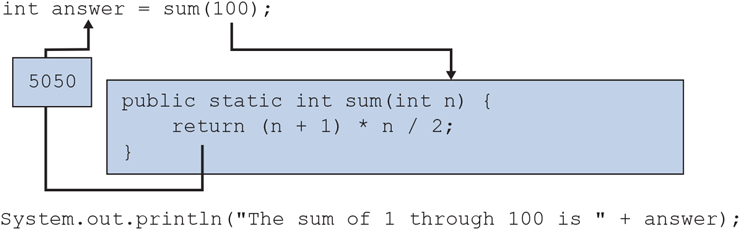
\includegraphics[width=\maxwidth,height=\maxheight,keepaspectratio,alt={Image}]{Figures/img_p44_0.png}}
\end{center}


\caption{Image}
\end{figure}

Một lần nữa, lưu ý rằng trong phần tiêu đề của phương thức, từ quen
thuộc \texttt{void} (chỉ ra rằng không có giá trị trả về) đã được thay
thế bằng từ \texttt{int}. Hãy nhớ rằng khi bạn khai báo một phương thức
trả về một giá trị, bạn phải báo cho Java biết loại giá trị nào nó sẽ
trả về. Do đó, chúng ta có thể cập nhật bản mẫu cú pháp của chúng ta cho
các phương thức tĩnh một lần nữa để làm rõ rằng phần tiêu đề bao gồm một
kiểu trả về (\texttt{void} cho không trả về):

\begin{verbatim}
public static <type> <name>(<type> <name>, ..., <type> <name>) 
{
    <statement>;
    <statement>;
    ...
    <statement>;
}
\end{verbatim}

Cú pháp của câu lệnh \texttt{return} là:

\begin{verbatim}
return <expression>;
\end{verbatim}

Khi Java gặp một câu lệnh \texttt{return}, nó tính toán biểu thức đã cho
và ngay lập tức kết thúc phương thức, trả về giá trị mà nó nhận được từ
biểu thức đó. Do đó, việc có bất kỳ câu lệnh nào khác sau một câu lệnh
\texttt{return} là không hợp lệ; \texttt{return} phải là câu lệnh cuối
cùng trong phương thức của bạn. Việc một phương thức Java có kiểu trả về
khác \texttt{void} kết thúc mà không có một lệnh \texttt{return} cũng là
một lỗi.

Có những ngoại lệ đối với các quy tắc trước đó, như bạn sẽ thấy sau này.
Ví dụ, việc một phương thức có nhiều hơn một câu lệnh \texttt{return} là
có thể xảy ra; điều này sẽ được đề cập trong chương tiếp theo, khi chúng
ta thảo luận về việc thực thi có điều kiện bằng các câu lệnh \texttt{if}
và \texttt{if/else}.

Hãy xem một phương thức mẫu khác có trả về một giá trị. Trong \emph{The
Wizard of Oz}, Bù Nhìn (Scarecrow) sau khi được cấp bằng tốt nghiệp đã
thể hiện sự thông minh của mình bằng cách mô tả một công thức sử dụng
tổng các căn bậc hai của hai cạnh bất kỳ của một tam giác cân. Có lẽ anh
ta đang cố gắng phát biểu định lý Pythagoras, mặc dù không rõ liệu những
người viết kịch bản dở toán hay họ đang đưa ra bình luận về giá trị của
một tấm bằng tốt nghiệp. Trong một tập phim của \emph{The Simpsons},
Homer lặp lại công thức sai lầm của Bù Nhìn sau khi đeo một cặp kính của
Henry Kissinger mà anh tìm thấy trong nhà vệ sinh tại nhà máy điện hạt
nhân Springfield.

Định lý Pythagoras chính xác chỉ áp dụng cho các tam giác vuông và phát
biểu rằng độ dài của cạnh huyền của một tam giác vuông bằng căn bậc hai
của tổng bình phương hai cạnh còn lại. Nếu bạn biết độ dài của hai cạnh
\(a\) và \(b\) của một tam giác vuông và muốn tìm độ dài của cạnh thứ ba
\(c\), bạn tính nó như sau: \(c = \sqrt{a^2 + b^2}\)

\begin{quote}
\textbf{LỖI LẬP TRÌNH PHỔ BIẾN (COMMON PROGRAMMING ERROR)}

\textbf{Bỏ qua Giá trị được Trả về (Ignoring the Returned Value)}

Khi bạn gọi một phương thức trả về một giá trị, kỳ vọng là bạn sẽ làm gì
đó với giá trị được trả về đó. Bạn có thể in nó ra, lưu nó vào một biến,
hoặc sử dụng nó như một phần của một biểu thức lớn hơn. Việc gọi phương
thức và chỉ đơn giản bỏ qua giá trị được trả về từ nó là hợp lệ (nhưng
không khôn ngoan):

\begin{verbatim}
sum(1000);   // doesn’t do anything
\end{verbatim}

Lời gọi ở trên không in ra tổng số cũng như không có bất kỳ tác dụng
đáng chú ý nào. Nếu bạn muốn giá trị được in ra, bạn phải bao gồm một
câu lệnh \texttt{println}:

\begin{verbatim}
int answer = sum(1000);    // better
System.out.println("Sum up to 1000 is " + answer);
\end{verbatim}

Một dạng ngắn hơn của đoạn mã đã sửa sẽ như sau:

\begin{verbatim}
System.out.println("Sum up to 1000 is " + sum(1000));
\end{verbatim}
\end{quote}

Giả sử bạn muốn in ra độ dài của các cạnh huyền của hai tam giác vuông,
một tam giác có độ dài các cạnh là 5 và 12, và tam giác còn lại có độ
dài các cạnh là 3 và 4. Bạn có thể viết đoạn mã như sau:

\begin{verbatim}
double c1 = Math.sqrt(Math.pow(5, 2) + Math.pow(12, 2));
System.out.println("hypotenuse 1 = " + c1);
double c2 = Math.sqrt(Math.pow(3, 2) + Math.pow(4, 2));
System.out.println("hypotenuse 2 = " + c2);
\end{verbatim}

Đoạn mã trước đó là chính xác, nhưng hơi khó đọc, và bạn sẽ phải lặp lại
cùng một phép toán phức tạp đó lần thứ ba nếu bạn muốn bao gồm một tam
giác thứ ba. Một giải pháp tốt hơn sẽ là tạo ra một phương thức để tính
toán và trả về độ dài cạnh huyền khi được truyền độ dài của hai cạnh kia
dưới dạng các tham số. Một phương thức như vậy sẽ trông giống như thế
này:

\begin{verbatim}
public static double hypotenuse(double a, double b) { 
    double c = Math.sqrt(Math.pow(a, 2) + Math.pow(b, 2)); 
    return c; 
}
\end{verbatim}

Phương thức này có thể được sử dụng để tạo ra một phương thức
\texttt{main} ngắn gọn và dễ đọc hơn, như được hiển thị dưới đây.

\begin{verbatim}
1  // Computes triangle hypotenuse lengths using return values. 
2  public class Triangles { 
3      public static void main(String[] args) { 
4          System.out.println("hypotenuse 1 = " + hypotenuse(5, 12)); 
5          System.out.println("hypotenuse 2 = " + hypotenuse(3, 4)); 
6      } 
7 
8      public static double hypotenuse(double a, double b) { 
9          double c = Math.sqrt(Math.pow(a, 2) + Math.pow(b, 2)); 
10         return c; 
11     } 
12 }
\end{verbatim}

Một số biến thể của chương trình này là có thể thực hiện. Thứ nhất,
không cần thiết phải lưu giá trị trả về của phương thức
\texttt{hypotenuse} vào biến \texttt{c}. Nếu muốn, bạn chỉ cần tính toán
và trả về giá trị đó trong một dòng duy nhất. Trong trường hợp này, phần
thân của phương thức \texttt{hypotenuse} sẽ trở thành như sau:

\begin{verbatim}
return Math.sqrt(Math.pow(a, 2) + Math.pow(b, 2));
\end{verbatim}

Ngoài ra, một số lập trình viên tránh sử dụng \texttt{Math.pow} đối với
các số mũ thấp như 2 và chỉ thực hiện phép nhân thủ công. Sử dụng cách
tiếp cận đó, phần thân của phương thức \texttt{hypotenuse} sẽ trông
giống như thế này:

\begin{verbatim}
return Math.sqrt(a * a + b * b);
\end{verbatim}

\begin{quote}
\textbf{LỖI LẬP TRÌNH PHỔ BIẾN (COMMON PROGRAMMING ERROR)}

\textbf{Câu lệnh sau lệnh Return (Statement after Return)}

Sẽ là không hợp lệ khi đặt các câu lệnh khác ngay sau một câu lệnh
\texttt{return}, bởi vì các câu lệnh đó không bao giờ có thể tiếp cận
tới được hay thực thi được. Các lập trình viên mới thường vô tình làm
điều này khi cố gắng in giá trị của một biến sau khi trả về. Giả sử bạn
đã viết phương thức \texttt{hypotenuse} nhưng vô tình viết các tham số
cho \texttt{Math.pow} theo sai thứ tự, do đó phương thức không tạo ra
câu trả lời đúng. Bạn
\end{quote}

\begin{quote}
có thể viết như sau, với ý định in ra kết quả trước khi trả về nó:

\begin{verbatim}
public static double hypotenuse(double a, double b) {
    double c = Math.sqrt(Math.pow(b, 2) + Math.pow(a, 2));
    return c;
    System.out.println("c is " + c); // ERROR!
}
\end{verbatim}

Bởi vì bạn muốn in giá trị của \texttt{c} trước khi trả về nó, bạn phải
đặt câu lệnh \texttt{println} trước lệnh \texttt{return}:

\begin{verbatim}
public static double hypotenuse(double a, double b) {
    double c = Math.sqrt(Math.pow(b, 2) + Math.pow(a, 2));
    System.out.println("c is " + c);
    return c;
}
\end{verbatim}
\end{quote}

\subsubsection{Thay đổi Giá trị của Biến (Changing a Variable's
Value)}\label{thay-ux111ux1ed5i-giuxe1-trux1ecb-cux1ee7a-biux1ebfn-changing-a-variables-value}

Có rất nhiều điều cần chú ý khi học cách sử dụng các tham số và giá trị
trả về một cách kết hợp với nhau. Chúng ta hãy xem xét một kịch bản đơn
giản nhằm làm nổi bật một số sai lầm phổ biến mà những người mới học mắc
phải.

Cú pháp truyền và thao tác với các biến như là tham số có thể khiến một
số người cho rằng việc thiết lập (setup) một tham số sẽ tạo ra mối liên
kết vĩnh viễn với biến ban đầu. Bạn đã thấy trước đây với các tham số,
phương thức chỉ được truyền một \emph{bản sao} của biến; do đó, phương
thức không thể thay đổi giá trị của biến thông qua tham số.

Ví dụ, giả sử bạn đang phát triển một chương trình trong đó bạn muốn yêu
cầu người dùng xác định điểm \(x\) và \(y\). Bạn muốn bắt đầu chúng bằng
0 và sau đó sử dụng một phương thức để sửa đổi tọa độ của chúng:

\begin{verbatim}
// Sets x and y to specific values.
// Doesn't work; x and y are passed by value and only copied.
public class PointSet {
    public static void main(String[] args) {
        int x = 0;
        int y = 0;
        setPoint(x, y);
        System.out.println("x = " + x + ", y = " + y);
    }
    
    public static void setPoint(int x, int y) {
        x = 9;
        y = 2;
    }
}
\end{verbatim}

Kết quả đầu ra của chương trình này là \texttt{x\ =\ 0,\ y\ =\ 0}. Mặc
dù tên của các tham số trùng khớp với tên của các biến cục bộ trong
\texttt{main}, chúng đại diện cho các giá trị riêng biệt. Phương thức
\texttt{main} và phương thức \texttt{setPoint} không giao tiếp với nhau.
Do đó, các thay đổi đối với tham số của \texttt{setPoint} không có tác
dụng đối với các biến cục bộ của \texttt{main}.

\begin{quote}
\textbf{Chỉ báo Giá trị so với Biến (Value versus Variable Semantics)}

Các tham số của các kiểu dữ liệu nguyên thủy (primitive) (như
\texttt{int} và \texttt{double}) được truyền theo \emph{giá trị}
(value). Phương thức nhận được một bản sao của giá trị được truyền, và
bất kỳ thay đổi nào thực hiện đối với tham số này đều không tác động đến
biến ban đầu.
\end{quote}

Làm thế nào chúng ta có thể truyền dữ liệu từ \texttt{setPoint} trở lại
\texttt{main}? Một biến cục bộ của phương thức \texttt{main} không thể
bị một phương thức khác thay đổi trừ khi bạn trả về giá trị mới và lưu
trữ (gán) nó vào biến đó.

Ví dụ, bạn có thể thực hiện tính toán giá trị một cách tách biệt hoặc
định nghĩa hai phương thức riêng biệt, mỗi phương thức sẽ trả về một tọa
độ. Tuy nhiên, một phương thức Java không thể trả về hai giá trị cùng
một lúc. Giải pháp tốt hơn là sử dụng kỹ thuật lập trình hướng đối tượng
(object-oriented), chúng ta sẽ thấy ở Chương 8 khi giới thiệu các đối
tượng \texttt{Point} trong Java.

Một vấn đề phổ biến khác liên quan đến việc cập nhật biến trong cùng một
phương thức. Xét đoạn mã cố gắng tăng gấp đôi giá trị của một biến:

\begin{verbatim}
public class DoubleVariable {
    public static void main(String[] args) {
        int x = 5;
        doubleValue(x);
        System.out.println("x = " + x);
    }
    
    public static int doubleValue(int x) {
        return x * 2;
    }
}
\end{verbatim}

Kết quả đầu ra là \texttt{x\ =\ 5}. Lý do là mặc dù \texttt{doubleValue}
đã tính toán chính xác và trả về giá trị gấp đôi (10), nhưng giá trị này
không bao giờ được lưu. Dòng \texttt{doubleValue(x);} tính toán giá trị
\texttt{10}, nhưng sau đó ném nó đi.

Để sửa lỗi này, chúng ta cần gán kết quả trả về của phương thức cho một
biến:

\begin{verbatim}
int result = doubleValue(x);
\end{verbatim}

Hoặc, nếu chúng ta muốn thay đổi chính biến \texttt{x}, chúng ta có thể
gán giá trị mới lại cho biến \texttt{x} ban đầu:

\begin{verbatim}
x = doubleValue(x);
\end{verbatim}

\begin{verbatim}
int x = 8;
\end{verbatim}

bạn có thể viết

\begin{verbatim}
String s = "hello there";
\end{verbatim}

Bạn có thể khai báo các biến có kiểu \texttt{String} và sử dụng lệnh gán
để cung cấp giá trị cho các biến này. Bạn cũng có thể viết mã liên quan
đến các biểu thức \texttt{String}:

\begin{verbatim}
String s1 = "hello"; 
String s2 = "there"; 
String combined = s1 + " " + s2;
\end{verbatim}

Đoạn mã này định nghĩa hai \texttt{String}, mỗi chuỗi đại diện cho một
từ đơn lẻ và một \texttt{String} thứ ba đại diện cho việc nối
(concatenation) hai từ với một khoảng trắng ở giữa. Bạn sẽ nhận thấy
rằng kiểu \texttt{String} được viết hoa (giống như tên của tất cả các
kiểu đối tượng trong Java), không giống như các kiểu dữ liệu nguyên thủy
(primitive) như \texttt{double} và \texttt{int}.

Những ví dụ này chưa cho thấy điều gì đặc biệt về các đối tượng
\texttt{String}, nhưng chúng ta đang đi đến phần đó. Hãy nhớ rằng ý
tưởng đằng sau các đối tượng là bao gồm các thao tác cơ bản (basic
operations) đi kèm với chính dữ liệu, theo cách chúng ta tạo ra những
chiếc ô tô có tích hợp sẵn các bộ điều khiển. Dữ liệu được lưu trữ trong
một \texttt{String} là một chuỗi các ký tự (sequence of characters). Có
đủ loại thao tác mà bạn có thể muốn thực hiện trên chuỗi các ký tự này.
Ví dụ, bạn có thể muốn biết có bao nhiêu ký tự trong \texttt{String} đó.
Các đối tượng \texttt{String} có một phương thức \texttt{length} trả về
thông tin này.

Nếu phương thức \texttt{length} là tĩnh (static), bạn sẽ gọi nó bằng
cách viết đại loại như

\begin{verbatim}
length(s)     // this isn't legal
\end{verbatim}

Nhưng khi bạn thực hiện các thao tác trên các đối tượng, bạn sử dụng một
cú pháp khác. Các đối tượng lưu trữ dữ liệu và các phương thức, do đó
phương thức để báo cáo chiều dài (length) của một \texttt{String} thực
sự tồn tại bên trong chính đối tượng \texttt{String} đó. Để gọi phương
thức của một đối tượng, bạn viết tên của biến trước, theo sau là một dấu
chấm, và sau đó là tên của phương thức:

\begin{verbatim}
s.length()
\end{verbatim}

Hãy coi điều này như việc đang nói chuyện với đối tượng \texttt{String}.
Khi bạn yêu cầu \texttt{s.length()}, bạn đang nói, ``Này, \texttt{s}.
Tôi đang nói chuyện với bạn đây. Chiều dài của bạn là bao nhiêu?'' Tất
nhiên, các đối tượng \texttt{String} khác nhau có chiều dài khác nhau,
do đó bạn sẽ nhận được các câu trả lời khác nhau khi bạn giao tiếp với
các đối tượng \texttt{String} khác nhau.

Cú pháp chung để gọi một phương thức của một đối tượng như sau:

\begin{verbatim}
<variable>.<method name>(<expression>, <expression>, ..., <expression>)
\end{verbatim}

Ví dụ, tương tác JShell sau đây tạo ra hai biến \texttt{String} và hỏi
mỗi biến về chiều dài của nó:

\begin{verbatim}
jshell> String s1 = "hello";
s1 ==> "hello"
jshell> String s2 = "how are you?";
s2 ==> "how are you?"
jshell> s1.length()
$3 ==> 5
jshell> s2.length()
$4 ==> 12
\end{verbatim}

Bạn có thể muốn làm gì khác với một đối tượng \texttt{String} nữa? Với
phương thức \texttt{length}, bạn có thể tìm ra có bao nhiêu ký tự trong
một \texttt{String}, nhưng còn việc lấy ra từng ký tự (individual
characters) riêng lẻ thì sao? Có một vài cách để thực hiện điều này,
nhưng một trong những cách phổ biến nhất là sử dụng một phương thức tên
là \texttt{charAt}, nó trả về ký tự tại một vị trí cụ thể trong chuỗi.

Điều này dẫn chúng ta đến vấn đề về cách xác định vị trí trong một chuỗi
(sequence). Rõ ràng là có ký tự thứ nhất, ký tự thứ hai, v.v., vì vậy
việc sử dụng một số nguyên để dẫn chiếu đến một vị trí cụ thể là điều
hợp lý. Chúng ta gọi đây là chỉ số (index).

\begin{quote}
\textbf{Chỉ số (Index)}

Một số nguyên được sử dụng để chỉ định một vị trí trong một chuỗi các
giá trị. Java nói chung sử dụng việc đánh chỉ số dựa trên số không
(zero-based indexing) (với 0 là giá trị chỉ số đầu tiên, tiếp theo là 1,
2, 3, v.v.).
\end{quote}

Mỗi ký tự của một đối tượng \texttt{String} được gán một giá trị chỉ số,
bắt đầu bằng \texttt{0}. Ví dụ, đối với biến \texttt{s1} tham chiếu đến
chuỗi \texttt{"hello"}, các chỉ số là:

Có vẻ trực quan khi coi chữ cái ``h'' nằm ở vị trí thứ 1, nhưng có những
lợi thế khi bắt đầu với một chỉ số là 0. Đó là một quy ước đã được các
nhà thiết kế ngôn ngữ C áp dụng và được các nhà thiết kế của C++ và Java
làm theo, vì vậy đó là một quy ước bạn sẽ phải học cách sống chung với
nó.

Đối với \texttt{String} dài hơn là \texttt{s2}, các vị trí là:

Lưu ý rằng các khoảng trắng trong \texttt{String} này cũng có các vị trí
(ở đây là các vị trí thứ 3 và 7). Cũng xin lưu ý rằng các chỉ số cho một
chuỗi nhất định luôn có phạm vi từ 0 cho đến độ dài của chuỗi trừ đi
một.

Sử dụng phương thức \texttt{charAt}, bạn có thể yêu cầu các ký tự cụ thể
của một chuỗi. Kiểu trả về là \texttt{char}. Ví dụ, nếu bạn yêu cầu
\texttt{s1.charAt(1)} bạn sẽ nhận được
\texttt{\textquotesingle{}e\textquotesingle{}} (chữ `e' trong
``hello''). Nếu bạn yêu cầu \texttt{s2.charAt(5)}, bạn sẽ nhận được
\texttt{\textquotesingle{}r\textquotesingle{}} (chữ `r' trong ``how are
you?''). Đối với bất kỳ \texttt{String} nào, nếu bạn yêu cầu
\texttt{charAt(0)}, bạn sẽ nhận được ký tự đầu tiên của chuỗi đó.

Khi làm việc với các đối tượng \texttt{String}, bạn sẽ thường thấy hữu
ích khi viết một vòng lặp \texttt{for} để xử lý các ký tự khác nhau của
\texttt{String}. Vì các \texttt{String} được đánh chỉ số bắt đầu bằng
\texttt{0}, tác vụ này dễ viết hơn với các vòng lặp \texttt{for} bắt đầu
bằng \texttt{0} thay vì \texttt{1}. Lấy ví dụ, hãy xem xét tương tác
JShell sau đây, nó in ra từng ký tự riêng lẻ của \texttt{s1}:

\begin{verbatim}
jshell> String s1 = "hello"; 
s1 ==> "hello"
jshell> for (int i = 0; i < s1.length(); i++) {
   ...>     System.out.println(i + ": " + s1.charAt(i));
   ...> }
0: h
1: e
2: l
3: l
4: o
\end{verbatim}

Hãy nhớ rằng khi chúng ta bắt đầu các vòng lặp ở \texttt{0}, chúng ta
thường kiểm tra bằng toán tử nhỏ hơn (\texttt{\textless{}}) thay vì nhỏ
hơn hoặc bằng (\texttt{\textless{}=}). Chuỗi \texttt{s1} có năm ký tự
trong đó, do đó lời gọi tới \texttt{s1.length()} sẽ trả về \texttt{5}.
Nhưng vì chỉ số đầu tiên là \texttt{0}, chỉ số cuối cùng sẽ nhỏ hơn
\texttt{5} một đơn vị, tức là \texttt{4}. Quy ước này cần một thời gian
để làm quen, nhưng việc đánh chỉ số dựa trên số không được sử dụng xuyên
suốt trong Java, vì vậy cuối cùng bạn cũng sẽ nắm bắt được nó.

Một phương thức \texttt{String} hữu ích khác là phương thức
\texttt{substring}. Nó nhận vào hai đối số nguyên (integer arguments)
đại diện cho chỉ số bắt đầu và chỉ số kết thúc. Khi bạn gọi phương thức
\texttt{substring}, bạn cung cấp hai chỉ số này: chỉ số của ký tự đầu
tiên bạn muốn và chỉ số ngay sát sau chỉ số cuối cùng mà bạn muốn.

Hãy nhớ lại rằng \texttt{String} \texttt{s2} có các vị trí như sau:

Giả sử bạn muốn lấy ra các từ riêng lẻ từ chuỗi này. Để lấy từ đầu tiên,
``how'', bạn sẽ yêu cầu:

\begin{verbatim}
jshell> String s2 = "how are you?";
s2 ==> "how are you?"
jshell> s2.substring(0, 3)
$2 ==> "how"
\end{verbatim}

Hãy nhớ rằng giá trị thứ hai mà bạn truyền vào phương thức
\texttt{substring} được cho là sẽ nằm ngoài phần cuối của chuỗi con mà
bạn đang tạo ra một vị trí. Do đó, mặc dù có một khoảng trắng ở vị trí
thứ \texttt{3} trong chuỗi ban đầu, nó sẽ không phải là một phần của
những gì bạn nhận được từ lời gọi tới \texttt{substring}. Thay vào đó,
bạn sẽ nhận được tất cả các ký tự ngay trước vị trí thứ \texttt{3}.

Việc tuân theo quy tắc này có nghĩa là đôi khi bạn sẽ cung cấp một vị
trí cho một chuỗi con tại nơi mà không có ký tự nào. Ví dụ, ký tự cuối
cùng trong chuỗi mà \texttt{s2} tham chiếu tới nằm ở chỉ số \texttt{11}
(dấu chấm hỏi). Nếu bạn muốn lấy chuỗi con \texttt{"you?"} bao gồm cả
dấu chấm hỏi, bạn sẽ yêu cầu:

\begin{verbatim}
jshell> s2.substring(8, 12)
$3 ==> "you?"
\end{verbatim}

Không có ký tự nào ở vị trí \texttt{12} trong \texttt{s2}, nhưng lời gọi
này yêu cầu các ký tự bắt đầu ở vị trí \texttt{8} và xuất hiện trước vị
trí \texttt{12}, do đó điều này thực sự hợp lý.

Tuy nhiên, bạn phải cẩn thận về những chỉ số mà mình sử dụng. Với phương
thức \texttt{substring}, bạn có thể yêu cầu vị trí nằm ngay ngoài phần
cuối của chuỗi, nhưng bạn không thể yêu cầu bất cứ điều gì xa hơn thế.
Ví dụ, nếu bạn chỉ định \texttt{13} làm chỉ số kết thúc trong ví dụ
trước đó của chúng ta, mã sẽ tạo ra một lỗi thực thi (execution error):

\begin{verbatim}
jshell> s2.substring(8, 13)
|  java.lang.StringIndexOutOfBoundsException thrown:
|  begin 8, end 13, length 12
|        at String.checkBoundsBeginEnd (String.java:3107)
|        at String.substring (String.java:1873)
|        at (#4:1)
\end{verbatim}

Tương tự, nếu bạn yêu cầu \texttt{charAt} tại một vị trí không tồn tại,
chương trình của bạn sẽ tạo ra một lỗi thực thi. Những lỗi này được biết
đến như là các ngoại lệ (exceptions). Các ngoại lệ là các lỗi thời gian
chạy (runtime errors) như đã được đề cập trong Chương 1.

\begin{quote}
\textbf{Ngoại lệ (Exception)}

Một lỗi thời gian chạy (runtime error) ngăn cản chương trình tiếp tục
quá trình thực thi bình thường của nó.
\end{quote}

Chúng ta nói rằng một ngoại lệ bị ném ra (thrown) khi một lỗi gặp phải.
Khi một ngoại lệ bị ném ra, Java sẽ xem xét liệu bạn đã viết mã để xử lý
nó chưa. Nếu chưa, việc thực thi chương trình sẽ bị dừng lại và bạn sẽ
thấy những gì được gọi là dấu vết ngăn xếp (stack trace) hoặc dấu vết
lùi (back trace). Dấu vết ngăn xếp cho bạn thấy một chuỗi các phương
thức đã được gọi, theo thứ tự ngược lại. Trong trường hợp các chỉ số
\texttt{String} không hợp lệ, ngoại lệ sẽ in một thông báo như sau ra
giao diện điều khiển (console):

\begin{verbatim}
Exception in thread "main" 
        java.lang.StringIndexOutOfBoundsException: 
        String index out of range: 13 
        at java.lang.String.substring(Unknown Source) 
        at ExampleProgram.main(ExampleProgram.java:3)
\end{verbatim}

Bạn có thể sử dụng một \texttt{String} làm tham số cho phương thức. Ví
dụ, chương trình sau sử dụng các tham số \texttt{String} để in ra một
thông điệp tùy chỉnh cho một người dựa trên tên của họ:

\begin{verbatim}
 1  // This program demonstrates String parameters.
 2  public class FormLetter {
 3      public static void main(String[] args) {
 4          letter("Philip", "Smith");
 5          letter("Jean", "Geges");
 6      }
 7
 8      public static void letter(String first, String last) {
 9          System.out.println("Dear " + first + ",");
 10         System.out.println("Check out this amazing offer! 20%");
 11         System.out.println("off all items. A great deal, as");
 12         System.out.println("sure as your name is " + last + "!");
 13         System.out.println();
 14     }
 15  }
\end{verbatim}

Nó tạo ra kết quả đầu ra sau:

\begin{verbatim}
Dear Philip, 
Check out this amazing offer! 20% 
off all items. A great deal, as 
\end{verbatim}

sure as your name is Smith!

Dear Jean, Check out this amazing offer! 20\% off all items. A great
deal, as sure as your name is Geges!

\begin{verbatim}

Bảng 3.3 liệt kê một số phương thức hữu ích nhất mà bạn có thể gọi trên các đối tượng `String`.

**Bảng 3.3 Các Phương thức Hữu ích của Đối tượng String (Useful Methods of String Objects)**



Các chuỗi (`String`) trong Java là bất biến (immutable), điều đó có nghĩa là một khi chúng được khởi tạo, giá trị của chúng không bao giờ có thể bị thay đổi.

> **Đối tượng Bất biến (Immutable Object)**
>
> Một đối tượng mà giá trị của nó không thể bị thay đổi.

Có vẻ kỳ lạ khi các `String` là bất biến mà lại có các phương thức như `toUpperCase` và `toLowerCase`. Nhưng nếu bạn đọc kỹ các mô tả trong bảng, bạn sẽ thấy rằng các phương thức này thực sự không làm thay đổi một đối tượng `String` đã cho; thay vào đó, chúng trả về một chuỗi mới. Hãy xem xét đoạn mã sau:
```java
String s = "Hello, Maria";
s.toUpperCase();
System.out.println(s);
\end{verbatim}

Bạn có thể nghĩ rằng đoạn mã này sẽ biến chuỗi \texttt{s} thành chuỗi in
hoa tương đương của nó, nhưng không phải vậy. Dòng mã thứ hai tạo ra một
chuỗi mới có giá trị in hoa tương đương với giá trị của \texttt{s},
nhưng chúng ta không làm gì với giá trị mới này. Để biến chuỗi thành chữ
in hoa, chìa khóa là lưu chuỗi mới này vào một biến khác hoặc gán lại
biến \texttt{s} để nó trỏ tới chuỗi mới:

\begin{verbatim}
String s = "Hello, Maria";
s = s.toUpperCase();
System.out.println(s);
\end{verbatim}

Phiên bản mã này tạo ra kết quả đầu ra sau:

\begin{verbatim}
HELLO, MARIA
\end{verbatim}

Các phương thức \texttt{toUpperCase} và \texttt{toLowerCase} đặc biệt
hữu ích khi bạn muốn thực hiện so sánh các chuỗi mà trong đó bạn bỏ qua
việc viết hoa hay viết thường của các chữ cái liên quan.

Một phương thức hữu ích khác được tìm thấy trong các đối tượng
\texttt{String} là phương thức \texttt{replace}. Nó nhận hai tham số:
một chuỗi để tìm kiếm và một chuỗi mới để thay thế tất cả các lần xuất
hiện của chuỗi cần tìm đó bằng chuỗi mới.

Tương tác JShell sau đây trình diễn phương thức \texttt{replace}:

\begin{verbatim}
jshell> String name = "Tweedle Dee";
name ==> "Tweedle Dee"
jshell> name = name.replace("ee", "oo");
name ==> "Twoodle Doo"
jshell> name = name.replace("w", "");
name ==> "Toodle Doo"
\end{verbatim}

\subsection{Các Chương trình Tương tác và các Đối tượng Scanner
(Interactive Programs and Scanner
Objects)}\label{cuxe1c-chux1b0ux1a1ng-truxecnh-tux1b0ux1a1ng-tuxe1c-vuxe0-cuxe1c-ux111ux1ed1i-tux1b0ux1ee3ng-scanner-interactive-programs-and-scanner-objects}

Như bạn đã thấy, bạn có thể dễ dàng tạo ra kết quả đầu ra trong cửa sổ
giao diện điều khiển (console window) bằng cách gọi
\texttt{System.out.println} và \texttt{System.out.print}. Bạn cũng có
thể viết các chương trình tạm dừng và chờ người dùng gõ một phản hồi.
Các chương trình như vậy được biết đến như là các chương trình tương tác
(interactive programs), và các phản hồi do người dùng gõ vào được gọi là
đầu vào từ giao diện điều khiển (console input).

\begin{quote}
\textbf{Đầu vào Giao diện điều khiển (Console Input)}

Các phản hồi do người dùng gõ vào khi một chương trình tương tác tạm
dừng để chờ đầu vào.
\end{quote}

Khi bạn dẫn chiếu đến \texttt{System.out}, bạn đang truy cập vào một đối
tượng trong lớp \texttt{System} được gọi là luồng đầu ra tiêu chuẩn
(standard output stream), hoặc gọi tắt là ``standard out''. Có một đối
tượng tương ứng cho đầu vào tiêu chuẩn được gọi là \texttt{System.in},
nhưng Java không được thiết kế cho việc nhập vào từ giao diện điều khiển
và \texttt{System.in} chưa bao giờ đặc biệt dễ sử dụng cho mục đích này.

Thật may mắn cho chúng ta, có một cách dễ dàng hơn để đọc đầu vào từ
giao diện điều khiển: các đối tượng \texttt{Scanner}.

Hầu hết các đối tượng phải được khởi tạo một cách rõ ràng (explicitly
constructed) bằng cách gọi một phương thức đặc biệt được gọi là hàm khởi
tạo (constructor).

\begin{quote}
\textbf{Hàm khởi tạo (Khởi tạo) (Constructor (Construct))}

Một cú pháp đặc biệt được sử dụng để tạo và thiết lập các giá trị ban
đầu cho một đối tượng. Các đối tượng trong các chương trình Java phải
được khởi tạo trước khi chúng có thể được sử dụng.
\end{quote}

Hãy nhớ rằng một lớp giống như một bản thiết kế cho một họ các đối
tượng. Việc gọi một hàm khởi tạo giống như gửi một đơn đặt hàng đến nhà
máy yêu cầu nó làm theo bản thiết kế để cung cấp cho bạn một đối tượng
thực tế mà bạn có thể thao tác. Khi bạn gửi đơn đặt hàng của mình đến
nhà máy, đôi khi bạn sẽ chỉ định một số tham số nhất định (ví dụ: bạn
muốn đối tượng có màu gì).

Trong Java, các hàm khởi tạo được gọi bằng cách sử dụng từ khóa đặc biệt
\texttt{new}, theo sau là kiểu của đối tượng và bất kỳ tham số cần thiết
nào. Ví dụ, để khởi tạo một đối tượng \texttt{Scanner} cụ thể, bạn phải
truyền thông tin về nguồn của đầu vào. Cụ thể, bạn phải

cung cấp một luồng đầu vào (input stream). Để đọc từ cửa sổ giao diện
điều khiển, hãy truyền cho nó \texttt{System.in}:

\begin{verbatim}
Scanner console = new Scanner(System.in);
\end{verbatim}

Khi bạn đã khởi tạo xong đối tượng \texttt{Scanner}, bạn có thể yêu cầu
nó trả về một giá trị của một kiểu cụ thể. Một số phương thức, tất cả
đều bắt đầu bằng từ ``next'', có sẵn để lấy các kiểu giá trị khác nhau.
Bảng 3.4 liệt kê chúng.

\textbf{Bảng 3.4 Các Phương thức của Scanner (Scanner Methods)}

Thông thường, bạn sẽ sử dụng các biến để theo dõi các giá trị được trả
về bởi các phương thức này. Ví dụ, bạn có thể viết:

\begin{verbatim}
int n = console.nextInt();
\end{verbatim}

Lời gọi tới phương thức \texttt{nextInt} của đối tượng \texttt{console}
sẽ tạm dừng để chờ đầu vào của người dùng. Bất cứ khi nào máy tính tạm
dừng để chờ đầu vào, nó sẽ tạm dừng cho một dòng đầu vào hoàn chỉnh. Nói
cách khác, nó sẽ chờ cho đến khi người dùng nhấn phím Enter trước khi
tiếp tục thực thi chương trình.

Bạn có thể sử dụng lớp \texttt{Scanner} để đọc đầu vào từng dòng một
bằng cách sử dụng phương thức \texttt{nextLine}, mặc dù hiện tại chúng
ta sẽ không sử dụng \texttt{nextLine} nhiều lắm. Các phương thức
``next'' khác đều dựa trên thẻ bài (token-based) (nghĩa là chúng đọc các
phần tử riêng lẻ của đầu vào chứ không phải toàn bộ dòng).

\begin{quote}
\textbf{Thẻ bài (Token)}

Một phần tử riêng lẻ của đầu vào (ví dụ: một từ, một số).
\end{quote}

Theo mặc định, \texttt{Scanner} sử dụng khoảng trắng (whitespace) để
phân tách các thẻ bài.

\begin{quote}
\textbf{Khoảng trắng (Whitespace)}

Các dấu cách, các ký tự tab và các ký tự ngắt dòng.
\end{quote}

Một đối tượng \texttt{Scanner} xem xét những gì người dùng gõ vào và sử
dụng các khoảng trắng trên dòng đầu vào để chia nó thành các thẻ bài
riêng lẻ. Ví dụ, dòng đầu vào

\begin{verbatim}
hello     there. "how are"        "you?"  all-one-token
\end{verbatim}

sẽ được chia thành sáu thẻ bài:

\begin{verbatim}
hello
there.
"how
are"
"you?"
all-one-token
\end{verbatim}

Lưu ý rằng \texttt{Scanner} bao gồm các ký tự chấm câu (punctuation
characters) chẳng hạn như dấu chấm, dấu chấm hỏi và dấu ngoặc kép trong
các thẻ bài mà nó tạo ra. Nó cũng bao gồm cả dấu gạch ngang, vì vậy vì
không có khoảng trắng ở giữa để tách nó thành các thẻ bài khác nhau,
chúng ta chỉ nhận được một thẻ bài cho \texttt{"all-one-token"}. Việc
kiểm soát cách một \texttt{Scanner} biến mọi thứ thành các thẻ bài là
điều có thể thực hiện (một quá trình được gọi là tokenizing the input -
mã hóa đầu vào), nhưng chúng ta sẽ không làm bất cứ điều gì phức tạp như
thế.

Việc đọc nhiều hơn một giá trị từ một \texttt{Scanner} là có thể, như
trong:

\begin{verbatim}
double x = console.nextDouble();
double y = console.nextDouble();
\end{verbatim}

Vì có hai lời gọi khác nhau tới phương thức \texttt{nextDouble} của đối
tượng \texttt{console}, mã này sẽ khiến máy tính tạm dừng cho đến khi
người dùng đã nhập hai giá trị số. Các giá trị có thể được nhập trên
cùng một dòng hoặc trên các dòng riêng biệt. Nhìn chung, máy tính tiếp
tục tạm dừng để chờ đầu vào của người dùng cho đến khi nó đã lấy được
bất kỳ giá trị nào mà bạn đã yêu cầu \texttt{Scanner} lấy.

Nếu người dùng gõ vào một cái gì đó không phải là một số nguyên khi bạn
gọi \texttt{nextInt}, chẳng hạn như \texttt{XYZZY}, đối tượng
\texttt{Scanner} sẽ sinh ra một ngoại lệ. Hãy nhớ lại từ phần về các đối
tượng \texttt{String} rằng các ngoại lệ là những lỗi thời gian chạy làm
dừng việc thực thi chương trình. Trong trường hợp này, bạn sẽ thấy kết
quả lỗi thời gian chạy như sau:

\begin{verbatim}
Exception in thread "main" java.util.InputMismatchException 
        at java.util.Scanner.throwFor(Unknown Source) 
        at java.util.Scanner.next(Unknown Source) 
        at java.util.Scanner.nextInt(Unknown Source) 
        at Example.main(Example.java:13)
\end{verbatim}

Bạn sẽ thấy trong một chương sau cách để kiểm tra lỗi của người dùng.
Trong thời gian chờ đợi, chúng ta sẽ giả định rằng người dùng cung cấp
các đầu vào thích hợp.

\subsubsection{Chương trình Tương tác Mẫu (Sample Interactive
Program)}\label{chux1b0ux1a1ng-truxecnh-tux1b0ux1a1ng-tuxe1c-mux1eabu-sample-interactive-program}

Sử dụng lớp \texttt{Scanner}, chúng ta có thể viết một chương trình
tương tác hoàn chỉnh thực hiện một tính toán hữu ích cho người dùng. Nếu
bạn từng có ý định mua một ngôi nhà, bạn sẽ muốn biết khoản thanh toán
thế chấp hàng tháng của mình sẽ là bao nhiêu. Dưới đây là một chương
trình hoàn chỉnh hỏi thông tin về một khoản vay và in ra khoản thanh
toán hàng tháng:

\begin{verbatim}
 1   // This program prompts for information about a loan and
 2   // computes the monthly mortgage payment.
 3
 4   import java.util.*;   // for Scanner
 5
 6   public class Mortgage {
 7       public static void main(String[] args) {
 8           Scanner console = new Scanner(System.in);
 9
 10          // obtain values
 11          System.out.println("This program computes monthly " +
 12                             "mortgage payments.");
 13          System.out.print("loan amount    : ");
 14          double loan = console.nextDouble();
 15          System.out.print("number of years: ");
 16          int years = console.nextInt();
 17          System.out.print("interest rate  : ");
 18          double rate = console.nextDouble();
 19          System.out.println();
 20
 21          // compute result and report
 22          int n = 12 * years;
\end{verbatim}

\begin{verbatim}
 23          double c = rate / 12.0 / 100.0;
 24          double payment = loan * c * Math.pow(1 + c, n) /
 25                           (Math.pow(1 + c, n) - 1);
 26          System.out.println("payment = $" + (int) payment);
 27      }
 28  }
\end{verbatim}

Dưới đây là một quá trình thực thi mẫu của chương trình (đầu vào của
người dùng được in đậm):

\begin{verbatim}
This program computes monthly mortgage payments. 
loan amount    : 275000
number of years: 30
interest rate  : 4.25
 
payment = $1352
\end{verbatim}

Điều đầu tiên chúng ta làm trong chương trình là khởi tạo một đối tượng
\texttt{Scanner}, đối tượng mà chúng ta sẽ sử dụng cho đầu vào từ giao
diện điều khiển (console input). Tiếp theo, chúng ta giải thích những gì
chương trình sẽ làm, in ra một mô tả trên giao diện điều khiển. Điều này
là cần thiết đối với các chương trình tương tác. Bạn không muốn một
chương trình tạm dừng để chờ đầu vào của người dùng cho đến khi bạn đã
giải thích cho người dùng chuyện gì sắp xảy ra.

Bên dưới lệnh \texttt{println}, bạn sẽ nhận thấy có một số cặp câu lệnh
như sau:

\begin{verbatim}
System.out.print("loan amount     : ");
double loan = console.nextDouble();
\end{verbatim}

Câu lệnh đầu tiên được gọi là lời nhắc (prompt), một yêu cầu thông tin
từ người dùng. Chúng ta sử dụng một câu lệnh \texttt{print} thay vì
\texttt{println} để người dùng có thể gõ các giá trị trên cùng một dòng
với lời nhắc (tức là ở bên phải lời nhắc). Câu lệnh thứ hai gọi phương
thức \texttt{nextDouble} của đối tượng \texttt{console} để đọc một giá
trị có kiểu \texttt{double} từ người dùng. Giá trị này được lưu trong
một biến gọi là \texttt{loan}. Mẫu (pattern) các câu lệnh nhắc/đọc
(prompt/read) này rất phổ biến trong các chương trình tương tác.

Sau khi nhắc nhập các giá trị, chương trình sẽ tính toán một số giá trị.
Công thức tính khoản thanh toán thế chấp hàng tháng (monthly mortgage
payments) liên quan đến số tiền vay (loan amount), tổng số tháng tham
gia (một giá trị mà chúng ta gọi là \(n\)) và lãi suất hàng tháng
(monthly interest rate - một giá trị mà chúng ta gọi là \(c\)). Công
thức thanh toán được đưa ra bởi phương trình sau:

\(payment = \frac{loan \times c \times (1 + c)^n}{(1 + c)^n - 1}\)

Bạn sẽ nhận thấy trong chương trình, chúng ta sử dụng phương thức
\texttt{Math.pow} cho lũy thừa để chuyển đổi công thức này thành một
biểu thức Java.

Dòng cuối cùng của chương trình in ra khoản thanh toán hàng tháng. Bạn
có thể tưởng tượng rằng chúng ta chỉ cần viết:

\begin{verbatim}
System.out.println("payment = $" + payment);
\end{verbatim}

Tuy nhiên, vì khoản thanh toán được lưu trữ trong một biến kiểu
\texttt{double}, một câu lệnh như vậy sẽ in ra tất cả các chữ số của số
đó. Ví dụ, với nhật ký (log) được liệt kê ở trên, nó sẽ in ra như sau:

\begin{verbatim}
payment = $1352.8347004685593
\end{verbatim}

Đó là một kết quả đầu ra trông khá kỳ lạ đối với một người đã quen với
tiền đô la và tiền xu (cent). Vì mục đích của chương trình đơn giản này,
thật dễ dàng để ép kiểu (cast) biến \texttt{double} thành một biến
\texttt{int} và chỉ báo cáo số tiền đô la của khoản thanh toán:

\begin{verbatim}
System.out.println("payment = $" + (int) payment);
\end{verbatim}

Hầu hết những người đang cố gắng tính toán các khoản thanh toán thế chấp
của họ không quan tâm nhiều đến những đồng xu lẻ, do đó chương trình vẫn
hữu ích. Trong phần tiếp theo, chúng ta sẽ xem cách làm tròn một số
\texttt{double} đến hai chữ số thập phân.

Có một thứ mới ở phần đầu của tập tin lớp (class file) này được gọi là
khai báo nhập (import declaration). Hãy nhớ rằng Java có một lượng lớn
các lớp được bao gồm trong những gì được gọi chung là các thư viện lớp
Java (Java class libraries). Để giúp quản lý các lớp này, Java cung cấp
một đơn vị tổ chức được gọi là một gói (package). Các lớp có liên quan
được kết hợp lại với nhau vào một gói duy nhất. Ví dụ, lớp
\texttt{Scanner} được lưu trữ trong một gói có tên là
\texttt{java.util}. Các chương trình Java thông thường không có quyền
truy cập vào một gói trừ khi chúng bao gồm một khai báo nhập.

\begin{quote}
\textbf{Gói (Package)}

Một tập hợp các lớp Java có liên quan.

\textbf{Khai báo Nhập (Import Declaration)}

Một yêu cầu để truy cập một gói Java cụ thể.
\end{quote}

Chúng ta chưa cần đến một khai báo nhập nào cho đến nay bởi vì Java tự
động nhập mọi lớp được lưu trữ trong một gói có tên là
\texttt{java.lang}. Gói \texttt{java.lang} bao gồm các lớp cơ bản mà hầu
hết các chương trình Java có khả năng sử dụng (ví dụ: \texttt{System},
\texttt{String}, \texttt{Math}). Bởi vì Java không tự động nhập
\texttt{java.util}, bạn phải tự mình làm điều đó.

Java cho phép bạn sử dụng một dấu hoa thị (asterisk) để nhập tất cả các
lớp từ một gói:

\begin{verbatim}
import java.util.*;
\end{verbatim}

Nhưng một số người thích đề cập cụ thể đến từng lớp mà họ nhập. Khai báo
nhập cho phép bạn chỉ nhập một lớp duy nhất từ một gói, như trong:

\begin{verbatim}
import java.util.Scanner;
\end{verbatim}

Vấn đề là một khi bạn bắt đầu nhập một lớp từ một gói, bạn có thể sẽ
muốn nhập cả các lớp khác nữa. Chúng ta sẽ sử dụng phiên bản nhập dùng
dấu hoa thị trong cuốn sách này để giữ cho mọi thứ đơn giản.

\subsection{Nghiên cứu Điển hình: Quỹ đạo của Vật thể bay (Case
Study: Projectile
Trajectory)}\label{nghiuxean-cux1ee9u-ux111iux1ec3n-huxecnh-quux1ef9-ux111ux1ea1o-cux1ee7a-vux1eadt-thux1ec3-bay-case-study-projectile-trajectory}

Đã đến lúc tập hợp các luồng nội dung của chương này bằng một ví dụ phức
tạp hơn, ví dụ này sẽ liên quan đến các tham số, các phương thức trả về
các giá trị, các tính toán toán học và việc sử dụng đối tượng
\texttt{Scanner} cho đầu vào từ giao diện điều khiển.

Các sinh viên vật lý thường được yêu cầu tính toán quỹ đạo (trajectory)
mà một vật thể (projectile) sẽ bay theo, với vận tốc ban đầu và góc ban
đầu của nó so với phương ngang. Ví dụ, vật thể có thể là một quả bóng đá
mà ai đó vừa đá. Chúng बताए muốn tính toán đường đi của nó trong điều
kiện trọng lực của Trái đất. Để giữ cho phép tính toán hợp lý, chúng ta
sẽ bỏ qua sức cản của không khí.

Có một số câu hỏi liên quan đến bài toán này mà chúng ta có thể muốn trả
lời:

\begin{itemize}
\tightlist
\item
  Khi nào vật thể chạm đến điểm cao nhất của nó?
\item
  Nó bay cao đến mức nào?
\item
  Mất bao lâu để nó rơi trở lại mặt đất?
\item
  Nó rơi cách vị trí được phóng đi bao xa?
\end{itemize}

Có một số cách để trả lời những câu hỏi này. Một cách tiếp cận đơn giản
là cung cấp một bảng hiển thị quỹ đạo theo từng bước (step by step), chỉ
ra vị trí \(x\), vị trí \(y\) và thời gian trôi qua.

Để tạo ra một bảng như vậy, chúng ta cần lấy ba giá trị từ người dùng:
vận tốc ban đầu, góc so với phương ngang, và số bước cần đưa vào bảng mà
chúng ta sẽ tạo ra. Chúng ta có thể yêu cầu vận tốc tính bằng mét/giây
hoặc feet/giây, nhưng vì đây là một bài toán vật lý, chúng ta sẽ gắn bó
với hệ mét và yêu cầu tính bằng mét/giây.

Chúng ta cũng phải suy nghĩ về cách xác định góc. Đáng tiếc là, hầu hết
các phương thức Java thao tác trên các góc đều yêu cầu các góc tính bằng
radian chứ không phải độ. Chúng ta có thể yêu cầu góc tính bằng radian,
nhưng điều đó sẽ rất bất tiện cho người dùng, người sẽ phải thực hiện
phép chuyển đổi. Thay vào đó, chúng ta có thể cho phép người dùng nhập
góc tính bằng độ và sau đó chuyển đổi nó sang radian bằng cách sử dụng
phương thức tích hợp sẵn \texttt{Math.toRadians}.

Vì vậy, phần tương tác của chương trình sẽ trông giống như thế này:

\begin{verbatim}
Scanner console = new Scanner(System.in);
System.out.print("velocity (meters/second)? ");
double velocity = console.nextDouble();
System.out.print("angle (degrees)? ");
double angle = Math.toRadians(console.nextDouble());
System.out.print("number of steps to display? ");
int steps = console.nextInt();
\end{verbatim}

Lưu ý rằng đối với vận tốc và góc, chúng ta gọi phương thức
\texttt{nextDouble} của đối tượng \texttt{console}, vì chúng ta muốn cho
phép người dùng chỉ định bất kỳ số nào (bao gồm cả số có dấu thập phân),
nhưng đối với số bước, chúng ta gọi \texttt{nextInt}, vì số dòng trong
bảng của chúng ta cần phải là một số nguyên.

Hãy nhìn kỹ hơn vào dòng mã này:

\begin{verbatim}
double angle = Math.toRadians(console.nextDouble());
\end{verbatim}

Một số người mới bắt đầu sẽ viết nó thành hai bước riêng biệt:

\begin{verbatim}
double angleInDegrees = console.nextDouble();
double angle = Math.toRadians(angleInDegrees);
\end{verbatim}

Cả hai cách tiếp cận đều hoạt động và hợp lý, nhưng hãy nhớ rằng bạn
không cần chia thao tác này thành hai bước riêng biệt. Bạn có thể viết
nó dưới dạng gọn gàng hơn như là một dòng mã duy nhất.

Khi chúng ta đã lấy được những giá trị này từ người dùng, chúng ta đã
sẵn sàng để bắt đầu các phép tính toán cho bảng quỹ đạo. Vị trí \(x/y\)
của vật thể tại mỗi gia số thời gian (time increment) được xác định bởi
vận tốc của nó theo mỗi chiều và gia tốc tác dụng lên vật thể do trọng
lực. Hình 3.1 cho thấy vận tốc ban đầu \(v_0\) và góc \(\theta\) ngay
lúc vật thể được ném ra và vận tốc cuối cùng \(v_t\) ngay lúc nó chạm
đất.

\textbf{Hình 3.1 Vận tốc Ban đầu và Vận tốc Cuối cùng của Vật thể}

Chúng ta cần tính toán thành phần \(x\) của vận tốc so với thành phần
\(y\) của vận tốc. Từ vật lý học, chúng ta biết rằng chúng có thể được
tính toán như sau:

\begin{figure}
\centering


\begin{center}
\pandocbounded{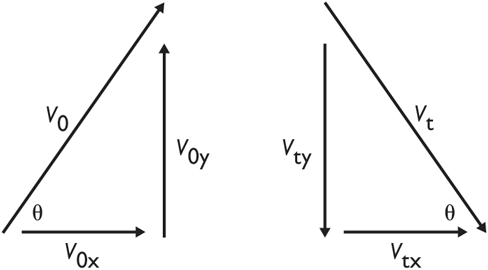
\includegraphics[width=\maxwidth,height=\maxheight,keepaspectratio,alt={Image}]{Figures/img_p83_1.png}}
\end{center}


\caption{Image}
\end{figure}

\begin{verbatim}
double xVelocity = velocity * Math.cos(angle);
double yVelocity = velocity * Math.sin(angle);
\end{verbatim}

Bởi vì chúng ta đang bỏ qua khả năng có sức cản của không khí, vận tốc
theo phương \(x\) sẽ không thay đổi. Tuy nhiên, vận tốc theo phương
\(y\) lại chịu lực hút của trọng lực. Vật lý học cho chúng ta biết rằng
trên bề mặt Trái đất, gia tốc do trọng lực xấp xỉ
\(9.81\text{ meters/second}^2\). Đây là một giá trị thích hợp để định
nghĩa thành một hằng số của lớp (class constant):

\begin{verbatim}
public static final double ACCELERATION = -9.81;
\end{verbatim}

Lưu ý rằng chúng ta định nghĩa gia tốc trọng lực là một số âm bởi vì nó
làm giảm vận tốc theo phương \(y\) của một vật thể (kéo nó xuống thay vì
đẩy nó lên).

Mục tiêu của chúng ta là hiển thị các giá trị \(x\), \(y\) và thời gian
trôi qua khi vật thể bay lên và sau đó rơi xuống. Vận tốc theo phương
\(y\) giảm dần cho đến khi nó bằng \(0\). Từ vật lý học, chúng ta biết
rằng đồ thị của vật thể sẽ đối xứng. Vật thể sẽ bay lên trên cho đến khi
vận tốc theo phương \(y\) của nó đạt tới \(0\), và sau đó nó sẽ theo một
đường đi tương tự rơi trở xuống trong một khoảng thời gian bằng nhau. Do
đó, tổng thời gian tính bằng giây có thể được tính như sau:

\begin{verbatim}
double totalTime = -2.0 * yVelocity / ACCELERATION;
\end{verbatim}

Bây giờ, làm thế nào để chúng ta tính toán các giá trị của \(x\), \(y\)
và thời gian trôi qua để đưa vào bảng của chúng ta? Việc tính toán hai
trong số này là tương đối đơn giản. Chúng ta muốn có các khoảng gia số
thời gian (time increments) đều đặn cho mỗi mục nhập trong bảng, do đó
chúng ta có thể tính toán gia số thời gian bằng cách chia tổng thời gian
cho số bước chúng ta muốn đưa vào bảng của mình:

\begin{verbatim}
double timeIncrement = totalTime / steps;
\end{verbatim}

Như đã lưu ý ở trên, vận tốc theo phương \(x\) không thay đổi, vì vậy
đối với mỗi khoảng gia số thời gian này, chúng ta di chuyển cùng một
khoảng cách theo hướng \(x\):

\begin{verbatim}
double xIncrement = xVelocity * timeIncrement;
\end{verbatim}

Giá trị khó để tính toán ở đây là vị trí \(y\). Vì gia tốc do trọng lực,
vận tốc theo phương \(y\) thay đổi theo thời gian. Nhưng từ vật lý học,
chúng ta có công thức tổng quát sau để tính toán độ dời (displacement)
của một vật thể với vận tốc \(v\), thời gian \(t\) và gia tốc \(a\):

\(displacement = v t + \frac{1}{2} a t^2\)

Trong trường hợp của chúng ta, vận tốc chúng ta muốn là vận tốc theo
phương \(y\) và gia tốc là từ hằng số trọng lực của Trái đất. Do đó, đây
là một mô tả bằng mã giả (pseudocode) về cách tạo ra bảng:

\begin{verbatim}
thiết lập tất cả x, y, và t bằng 0.
for (số bước đã cho) {
    cộng thêm timeIncrement vào t.
    cộng thêm xIncrement vào x.
    đặt lại y thành yVelocity * t + 0.5 * ACCELERATION * t * t.
    báo cáo số bước (step #), x, y, t.
}
\end{verbatim}

Chúng ta đã khá gần với việc có mã Java thực sự ở đây, nhưng chúng ta
phải suy nghĩ về cách báo cáo các giá trị của \(x\), \(y\) và \(t\)
trong một bảng. Chúng đều sẽ có kiểu \texttt{double}, điều đó có nghĩa
là chúng có khả năng tạo ra một lượng lớn các chữ số sau dấu thập phân.
Nhưng chúng ta không muốn nhìn thấy tất cả các chữ số đó, vì chúng không
đặc biệt liên quan và vì các tính toán của chúng ta không chính xác đến
mức đó.

Trước khi chúng ta cố gắng hoàn thành đoạn mã cho bảng, hãy nghĩ về vấn
đề hiển thị chỉ một số chữ số của một số. Ý tưởng là cắt bớt (truncate)
các chữ số để chúng ta không nhìn thấy tất cả chúng. Một cách để cắt bớt
là ép kiểu một số \texttt{double} thành một số \texttt{int}, thao tác
này sẽ cắt bớt tất cả các chữ số sau dấu thập phân. Chúng ta có thể làm
điều đó, nhưng chúng ta có lẽ muốn giữ lại ít nhất một số chữ số trong
đó. Ví dụ, giả sử rằng chúng ta muốn báo cáo hai chữ số sau dấu thập
phân. Thủ thuật (trick) ở đây là đưa hai chữ số mà chúng ta muốn sang
phía bên kia của dấu thập phân. Chúng ta có thể làm điều đó bằng cách
nhân với 100 và sau đó ép kiểu sang \texttt{int}:

\begin{verbatim}
(int) (n * 100.0)
\end{verbatim}

Biểu thức này mang lại cho chúng ta các chữ số mà chúng ta muốn, nhưng
bây giờ dấu thập phân nằm sai chỗ. Ví dụ, nếu \(n\) ban đầu là
\(3.488834\), biểu thức trên sẽ cho chúng ta \(348\). Chúng ta phải chia
kết quả này cho 100 để biến nó trở lại thành số \(3.48\):

\begin{verbatim}
(int) (n * 100.0) / 100.0
\end{verbatim}

Trong khi đang làm việc này, chúng ta có thể thực hiện một cải tiến cuối
cùng. Lưu ý rằng số ban đầu là \(3.488834\). Nếu chúng ta cắt bớt đơn
giản, chúng ta nhận được \(3.48\), nhưng thực sự số này gần với \(3.49\)
hơn. Chúng ta có thể làm tròn đến chữ số gần nhất bằng cách gọi phương
thức \texttt{Math.round} trên số đó thay vì ép kiểu nó:

\begin{verbatim}
Math.round(n * 100.0) / 100.0
\end{verbatim}

Đây là một thao tác mà chúng ta có khả năng sẽ muốn thực hiện trên nhiều
hơn một con số, vì vậy nó xứng đáng được đưa vào trong một phương thức:

\begin{verbatim}
public static double round2(double n) {
    return Math.round(n * 100.0) / 100.0;
}
\end{verbatim}

Quay trở lại mã giả của chúng ta cho bảng, chúng ta có thể kết hợp các
lời gọi tới phương thức \texttt{round2} để tiến gần hơn một chút tới mã
Java thực tế:

\begin{verbatim}
thiết lập tất cả x, y, và t bằng 0.
for (số bước đã cho) {
    cộng thêm timeIncrement vào t.
    cộng thêm xIncrement vào x.
    đặt lại y thành yVelocity * t + 0.5 * ACCELERATION * t * t.
    báo cáo số bước (step #), round2(x), round2(y), round2(t).
}
\end{verbatim}

Sẽ rất tuyệt nếu các giá trị trong bảng được căn chỉnh. Để có được các
con số xếp thành hàng ngay ngắn, chúng ta sẽ phải sử dụng đầu ra có định
dạng (formatted output), điều mà chúng ta sẽ thảo luận trong Chương 4.
Hiện tại, chúng ta ít nhất có thể sắp xếp các con số thành các cột bằng
cách tách chúng bằng các ký tự tab. Hãy nhớ rằng trình tự thoát (escape
sequence) \texttt{\textbackslash{}t} đại diện cho một dấu tab duy nhất.

Nếu chúng ta định có một bảng với các cột, việc có một tiêu đề (header)
cho bảng cũng rất hợp lý. Và chúng ta có lẽ muốn đưa vào một dòng trong
bảng hiển thị điều kiện ban đầu, nơi \(x\), \(y\) và \(time\) đều bằng
\(0\). Do đó, chúng ta có thể mở rộng mã giả của mình thành mã Java sau:

\begin{verbatim}
double x = 0.0;
double y = 0.0;
double t = 0.0;
System.out.println("step\tx\ty\ttime");
System.out.println("0\t0.0\t0.0\t0.0");
for (int i = 1; i <= steps; i++) {
    t += timeIncrement;
    x += xIncrement;
    y = yVelocity * t + 0.5 * ACCELERATION * t * t;
    System.out.println(i + "\t" + round2(x) + "\t" +
                       round2(y) + "\t" + round2(t));
}
\end{verbatim}

\subsubsection{Giải pháp Không có Cấu trúc (Unstructured
Solution)}\label{giux1ea3i-phuxe1p-khuxf4ng-cuxf3-cux1ea5u-truxfac-unstructured-solution}

Chúng ta có thể ghép tất cả các phần này lại với nhau để tạo thành một
chương trình hoàn chỉnh. Trước tiên, hãy xem một phiên bản không có cấu
trúc bao gồm phần lớn mã trong phương thức \texttt{main}. Phiên bản này
cũng bao gồm một số câu lệnh \texttt{println} mới ở phần đầu để giới
thiệu ngắn gọn cho người dùng:

\begin{verbatim}
 1  // This program computes the trajectory of a projectile.
 2
 3  import java.util.*; // for Scanner
 4
\end{verbatim}

\begin{verbatim}
 5  public class Projectile {
 6      // constant for Earth acceleration in meters/second^2
 7      public static final double ACCELERATION = -9.81;
 8
 9      public static void main(String[] args) {
 10         Scanner console = new Scanner(System.in);
 11
 12         System.out.println("This program computes the");
 13         System.out.println("trajectory of a projectile given");
 14         System.out.println("its initial velocity and its");
 15         System.out.println("angle relative to the");
 16         System.out.println("horizontal.");
 17         System.out.println();
 18
 19         System.out.print("velocity (meters/second)? ");
 20         double velocity = console.nextDouble();
 21         System.out.print("angle (degrees)? ");
 22         double angle = Math.toRadians(console.nextDouble());
 23         System.out.print("number of steps to display? ");
 24         int steps = console.nextInt();
 25         System.out.println();
 26
 27         double xVelocity = velocity * Math.cos(angle);
 28         double yVelocity = velocity * Math.sin(angle);
 29         double totalTime = -2.0 * yVelocity / ACCELERATION;
 30         double timeIncrement = totalTime / steps;
 31         double xIncrement = xVelocity * timeIncrement;
 32
 33         double x = 0.0;
 34         double y = 0.0;
 35         double t = 0.0;
 36         System.out.println("step\tx\ty\ttime");
 37         System.out.println("0\t0.0\t0.0\t0.0");
 38         for (int i = 1; i <= steps; i++) {
 39             t += timeIncrement;
 40             x += xIncrement;
 41             y = yVelocity * t + 0.5 * ACCELERATION * t * t;
 42             System.out.println(i + "\t" + round2(x) + "\t" +
 43                                round2(y) + "\t" + round2(t));
 44         }
 45     }
 46
 47     public static double round2(double n) {
 48         return Math.round(n * 100.0) / 100.0;
 49     }
 50 }
\end{verbatim}

Dưới đây là một quá trình thực thi mẫu của chương trình:

\begin{verbatim}
This program computes the 
trajectory of a projectile given 
its initial velocity and its 
angle relative to the 
horizontal. 
velocity (meters/second)? 30  
angle (degrees)? 50  
number of steps to display? 10  
step    x        y        time 
0       0.0      0.0      0.0 
1       9.03     9.69     0.47 
2       18.07    17.23    0.94 
3       27.1     22.61    1.41 
4       36.14    25.84    1.87 
5       45.17    26.92    2.34 
6       54.21    25.84    2.81 
7       63.24    22.61    3.28 
8       72.28    17.23    3.75 
9       81.31    9.69     4.22 
10      90.35    0.0      4.69
\end{verbatim}

Từ nhật ký thực thi, bạn có thể thấy rằng vật thể đạt đến chiều cao tối
đa là 26.92 mét sau 2.34 giây (bước thứ năm) và nó rơi cách điểm xuất
phát 90.35 mét sau 4.69 giây (bước thứ mười).

Phiên bản này của chương trình hoạt động, nhưng chúng ta thường không
muốn đưa quá nhiều mã vào phương thức \texttt{main}. Phần tiếp theo sẽ
khám phá cách chia nhỏ chương trình thành các phần nhỏ hơn.

\subsubsection{Giải pháp Cấu trúc (Structured
Solution)}\label{giux1ea3i-phuxe1p-cux1ea5u-truxfac-structured-solution}

Có ba khối mã chính trong phương thức \texttt{main} của chương trình
\texttt{Projectile}: một chuỗi các câu lệnh \texttt{println} giới thiệu
chương trình cho người dùng, một chuỗi các câu lệnh nhắc người dùng nhập
ba giá trị được sử dụng để tạo bảng, và sau đó là mã tạo ra chính cái
bảng đó.

Do đó, trong mã giả, cấu trúc tổng thể trông giống như thế này:

\begin{verbatim}
đưa ra giới thiệu.
nhắc nhập vận tốc, góc, và số bước.
tạo ra bảng.
\end{verbatim}

Bước thứ nhất và bước thứ ba dễ dàng được chuyển thành các phương thức,
nhưng bước ở giữa thì không. Bước này nhắc người dùng nhập các giá trị
mà chúng ta cần để tạo ra bảng. Nếu chúng ta chuyển nó thành một phương
thức, nó sẽ phải bằng cách nào đó trả về ba giá trị lại cho
\texttt{main}. Một phương thức chỉ có thể trả về một giá trị duy nhất,
vì vậy thật không may chúng ta không thể chuyển bước này thành một
phương thức. Chúng ta có thể chuyển nó thành ba phương thức khác nhau,
một phương thức cho mỗi trong số ba giá trị, nhưng mỗi phương thức đó sẽ
chỉ dài hai dòng, vì vậy không rõ liệu làm như vậy có cải thiện cấu trúc
tổng thể hay không.

Do đó, cải tiến chính mà chúng ta có thể thực hiện là tách phần giới
thiệu và phần bảng thành các phương thức riêng biệt. Một cải tiến khác
mà chúng ta có thể thực hiện là biến công thức độ dời trong vật lý thành
phương thức của riêng nó. Việc biến các phương trình thành các phương
thức luôn là một ý tưởng hay. Đưa ra các phương thức đó, chúng ta có
phiên bản cấu trúc (structured version) sau đây của chương trình:

\begin{verbatim}
 1  // This program computes the trajectory of a projectile.
 2
 3  import java.util.*;     // for Scanner
 4
 5  public class Projectile2 {
 6      // constant for Earth acceleration in meters/second^2
 7      public static final double ACCELERATION = -9.81;
 8
 9      public static void main(String[] args) {
 10         Scanner console = new Scanner(System.in);
 11         giveIntro();
 12
 13         System.out.print("velocity (meters/second)? ");
 14         double velocity = console.nextDouble();
 15         System.out.print("angle (degrees)? ");
 16         double angle = Math.toRadians(console.nextDouble());
 17         System.out.print("number of steps to display? ");
 18         int steps = console.nextInt();
 19         System.out.println();
 20
\end{verbatim}

\begin{verbatim}
 21         printTable(velocity, angle, steps);
 22     }
 23
 24     // prints a table showing the trajectory of an object given
 25     // its initial velocity and angle and including the given
 26     // number of steps in the table
 27     public static void printTable(double velocity,
 28                                   double angle, int steps) {
 29         double xVelocity = velocity * Math.cos(angle);
 30         double yVelocity = velocity * Math.sin(angle);
 31         double totalTime = -2.0 * yVelocity / ACCELERATION;
 32         double timeIncrement = totalTime / steps;
 33         double xIncrement = xVelocity * timeIncrement;
 34
 35         double x = 0.0;
 36         double y = 0.0;
 37         double t = 0.0;
 38         System.out.println("step\tx\ty\ttime");
 39         System.out.println("0\t0.0\t0.0\t0.0");
 40         for (int i = 1; i <= steps; i++) {
 41             t += timeIncrement;
 42             x += xIncrement;
 43             y = displacement(yVelocity, t, ACCELERATION);
 44             System.out.println(i + "\t" + round2(x) + "\t" +
 45                                round2(y) + "\t" + round2(t));
 46         }
 47     }
 48
 49     // gives a brief introduction to the user
 50     public static void giveIntro() {
 51         System.out.println("This program computes the");
 52         System.out.println("trajectory of a projectile given");
 53         System.out.println("its initial velocity and its");
 54         System.out.println("angle relative to the");
 55         System.out.println("horizontal.");
 56         System.out.println();
 57     }
 58
 59     // returns the vertical displacement for a body given
 60     // initial velocity v, elapsed time t, and acceleration a
 61     public static double displacement(double v, double  t,
 62                                       double a){
 63         return  v * t + 0.5 * a * t * t;
 64     }
 65
 66     // rounds n to 2 digits after the decimal point
 67     public static double round2(double n) {
 68         return Math.round(n * 100.0) / 100.0;
 69     }
 70 }
\end{verbatim}

Phiên bản này thực thi theo cùng một cách như phiên bản trước đó.

\subsection{Tóm tắt Chương (Chapter
Summary)}\label{tuxf3m-tux1eaft-chux1b0ux1a1ng-chapter-summary}

Các phương thức có thể được viết để chấp nhận các tham số (parameters),
là tập hợp các đặc điểm phân biệt các thành viên khác nhau của một họ
các tác vụ. Các tham số cho phép các giá trị dữ liệu đi vào một phương
thức, điều này có thể thay đổi cách phương thức thực thi. Một phương
thức được khai báo với một tập hợp các tham số có thể thực hiện toàn bộ
một họ các tác vụ tương tự nhau thay vì chỉ một tác vụ duy nhất.

Khi các giá trị nguyên thủy như kiểu \texttt{int} hoặc \texttt{double}
được truyền vào như là các tham số, các giá trị của chúng được sao chép
vào phương thức. Các tham số nguyên thủy (primitive parameters) gửi các
giá trị vào một phương thức nhưng không gửi ra khỏi phương thức đó;
phương thức có thể sử dụng các giá trị dữ liệu nhưng không thể ảnh hưởng
đến giá trị của bất kỳ biến nào nằm ngoài nó.

Hai phương thức có thể có cùng tên nếu chúng khai báo các tham số khác
nhau. Điều này được gọi là nạp chồng (overloading).

Các phương thức có thể được viết để trả về các giá trị cho mã đang gọi
(calling code). Tính năng này cho phép một phương thức thực hiện một
phép tính phức tạp và sau đó cung cấp kết quả của nó trở lại cho mã đang
gọi. Kiểu của giá trị trả về phải được khai báo trong tiêu đề của phương
thức và được gọi là kiểu trả về (return type) của phương thức.

Java có một lớp tên là \texttt{Math} chứa một số phương thức tĩnh hữu
ích mà bạn có thể sử dụng trong các chương trình của mình, chẳng hạn như
lũy thừa, căn bậc hai, và logarit.

Một đối tượng (object) là một thực thể kết hợp dữ liệu và các thao tác.
Một số đối tượng trong Java bao gồm \texttt{String} (là chuỗi các ký tự
văn bản) và \texttt{Scanner} (chuyên đọc đầu vào của người dùng).

Các đối tượng chứa các phương thức hiện thực hóa các hành vi của chúng.
Để gọi một phương thức trên một đối tượng, hãy viết tên của đối tượng
đó, theo sau là một dấu chấm, theo sau là tên phương thức.

Một đối tượng \texttt{String} chứa một chuỗi các ký tự. Các ký tự có các
chỉ số (indexes), bắt đầu với \texttt{0} cho ký tự đầu tiên.

Ngoại lệ (exception) là một lỗi xảy ra khi một chương trình đã thực hiện
một hành động không hợp lệ và không thể tiếp tục thực thi bình thường.

Một số chương trình có tính tương tác và phản hồi đối với đầu vào từ
người dùng. Những chương trình này nên in một thông báo tới người dùng,
còn được gọi là lời nhắc (prompt), để yêu cầu nhập dữ liệu.

Java có một lớp tên là \texttt{Scanner} chuyên đọc đầu vào từ bàn phím.
Một đối tượng \texttt{Scanner} có thể đọc nhiều phần khác nhau của đầu
vào (còn được gọi là các thẻ bài) từ một nguồn đầu vào. Nó có thể đọc
từng thẻ bài một lần hoặc đọc toàn bộ một dòng tại một thời điểm.

\subsection{Bài tập Tự Kiểm tra (Self-Check
Problems)}\label{buxe0i-tux1eadp-tux1ef1-kiux1ec3m-tra-self-check-problems}

\subsubsection{Phần 3.1: Các Tham số
(Parameters)}\label{phux1ea7n-3.1-cuxe1c-tham-sux1ed1-parameters}

\textbf{1.} Cú pháp nào sau đây là chính xác cho một tiêu đề phương thức
có chứa các tham số?

\begin{enumerate}
\def\labelenumi{\alph{enumi}.}
\tightlist
\item
  \texttt{public\ static\ void\ example(x,\ y)\ \{}\strut \\
\item
  \texttt{public\ static\ (int\ x,\ int\ y)\ example()\ \{}\strut \\
\item
  \texttt{public\ static\ void\ example(int\ x,\ y)\ \{}\strut \\
\item
  \texttt{public\ static\ void\ example(x:\ int,\ y:\ int)\ \{}\strut \\
\item
  \texttt{public\ static\ void\ example(int\ x,\ int\ y)\ \{}
\end{enumerate}

\textbf{2.} Kết quả đầu ra do chương trình sau đây tạo ra là gì?

\begin{verbatim}
 1  public class MysteryNums {
 2      public static void main(String[] args) {
 3          int x = 15;
 4          sentence(x, 42);
 5
 6          int y = x - 5;
 7          sentence(y, x + y);
 8      }
 9
 10     public static void sentence(int num1, int num2) {
 11         System.out.println(num1 + " " + num2);
 12     }
 13  }
\end{verbatim}

\textbf{3.} Chương trình sau đây có 9 lỗi sai. Chúng là gì?

\begin{verbatim}
 1  public class Oops3 {
 2      public static void main() {
 3          double bubble = 867.5309;
 4          double x = 10.01;
 5          printer(double x, double y);
 6          printer(x);
 7          printer("barack", "obama");
 8          System.out.println("z = " + z);
 9      }
 10
 11     public static void printer(x, y double) {
 12         int z = 5;
 13         System.out.println("x = " + double x + " and y = " + y);
 14         System.out.println("The value from main is: " + bubble);
 15     }
 16  }
\end{verbatim}

\textbf{4.} Kết quả đầu ra do chương trình sau đây tạo ra là gì?

\begin{verbatim}
 1  public class Odds {
 2      public static void main(String[] args) {
 3          printOdds(3);
 4          printOdds(17 / 2);
 5
 6          int x = 25;
 7          printOdds(37 - x + 1);
 8      }
 9
 10     public static void printOdds(int n) {
 11         for (int i = 1; i <= n; i++) {
 12             int odd = 2 * i - 1;
 13             System.out.print(odd + " ");
 14         }
 15         System.out.println();
 16     }
 17  }
\end{verbatim}

\textbf{5.} Kết quả đầu ra của chương trình sau đây là gì?

\begin{verbatim}
 1   public class Weird {
 2      public static void main(String[] args) {
 3          int number = 8;
 4          halfTheFun(11);
 5          halfTheFun(2 - 3 + 2 * 8);
 6          halfTheFun(number);
 7          System.out.println("number = " + number);
 8      }
 9
 10     public static void halfTheFun(int number) {
 11         number = number / 2;
 12         for (int count = 1; count <= number; count++) {
\end{verbatim}

\begin{verbatim}
 13             System.out.print(count + " ");
 14         }
 15         System.out.println();
 16     }
 17  }
\end{verbatim}

\textbf{6.} Kết quả đầu ra của chương trình sau đây là gì?

\begin{verbatim}
 1  public class MysteryNumbers {
 2      public static void main(String[] args) {
 3          String one = "two";
 4          String two = "three";
 5          String three = "1";
 6          int number = 20;
 7
 8          sentence(one, two, 3);
 9          sentence(two, three, 14);
 10         sentence(three, three, number + 1);
 11         sentence(three, two, 1);
 12         sentence("eight", three, number / 2);
 13     }
 14
 15     public static void sentence(String three, String one, int number) {
 16         System.out.println(one + " times " + three + " = " + (number * 2));
 17     }
 18  }
\end{verbatim}

\textbf{7.} Kết quả đầu ra do chương trình sau đây tạo ra là gì?

\begin{verbatim}
 1  public class MysteryWho {
 2      public static void main(String[] args) {
 3          String whom = "her";
 4          String who = "him";
 5          String it = "who";
 6          String he = "it";
 7          String she = "whom";
 8
 9          sentence(he, she, it);
 10         sentence(she, he, who);
 11         sentence(who, she, who);
 12         sentence(it, "stu", "boo");
 13         sentence(it, whom, who);
 14     }
 15
 16     public static void sentence(String she, String who, String whom) {
 17         System.out.println(who + " and " + whom + " like " + she);
 18     }
 19  }
\end{verbatim}

\textbf{8.} Kết quả đầu ra do chương trình sau đây tạo ra là gì?

\begin{verbatim}
 1  public class MysteryTouch {
 2      public static void main(String[] args) {
 3          String head = "shoulders";
 4          String knees = "toes";
 5          String elbow = "head";
 6          String eye = "eyes and ears";
 7          String ear = "eye";
 8
 9          touch(ear, elbow);
 10         touch(elbow, ear);
 11         touch(head, "elbow");
 12         touch(eye, eye);
 13         touch(knees, "Toes");
 14         touch(head, "knees " + knees);
 15     }
 16
 17     public static void touch(String elbow, String ear) {
 18         System.out.println("touch your " + elbow + " to your " + ear);
 19     }
 20  }
\end{verbatim}

\textbf{9.} Kết quả đầu ra do chương trình sau đây tạo ra là gì?

\begin{verbatim}
 1  public class MysterySoda {
 2      public static void main(String[] args) {
 3          String soda = "Coke";
 4          String pop = "Pepsi";
 5          String Coke = "pop";
 6          String Pepsi = "soda";
 7          String say = pop;
 8
 9          carbonated(Coke, soda, pop);
 10         carbonated(pop, Pepsi, Pepsi);
 11         carbonated("pop", pop, "Kool-Aid");
 12         carbonated(say, "say", pop);
 13     }
 14
 15     public static void carbonated(String Coke, String soda, String pop) {
 16         System.out.println("say " + soda + " not " + pop + " or " + Coke);
 17     }
 18  }
\end{verbatim}

\textbf{10.} Viết một phương thức có tên là \texttt{printStrings} nhận
một tham số \texttt{String} và một tham số đại diện cho số lần lặp lại
và in ra \texttt{String} đó số lần đã cho với một khoảng trắng sau mỗi
lần. Ví dụ, lời gọi hàm

\begin{verbatim}
printStrings("abc", 5);
\end{verbatim}

sẽ in ra đầu ra sau:

\begin{verbatim}
abc abc abc abc abc
\end{verbatim}

\textbf{11.} Câu lệnh \texttt{System.out.println} hoạt động trên nhiều
kiểu giá trị khác nhau, chẳng hạn như số nguyên (integers) hoặc số thực
dấu phẩy động (doubles). Thuật ngữ dùng để gọi một phương thức như vậy
là gì?

\subsubsection{Phần 3.2: Các Phương thức Trả về Giá trị (Methods That
Return
Values)}\label{phux1ea7n-3.2-cuxe1c-phux1b0ux1a1ng-thux1ee9c-trux1ea3-vux1ec1-giuxe1-trux1ecb-methods-that-return-values}

\textbf{12.} Có gì sai với chương trình sau đây?

\begin{verbatim}
 1  public class Temperature {
 2      public static void main(String[] args) {
 3          double tempf = 98.6;
 4          double tempc = 0.0;
 5          ftoc(tempf, tempc);
 6          System.out.println("Body temp in C is: " + tempc);
 7      }
 8
 9      // converts Fahrenheit temperatures to Celsius
 10     public static void ftoc(double tempf, double tempc) {
 11         tempc = (tempf - 32) * 5 / 9;
 12     }
 13  }
\end{verbatim}

\textbf{13.} Đánh giá các biểu thức sau:

\begin{enumerate}
\def\labelenumi{\alph{enumi}.}
\tightlist
\item
  \texttt{Math.abs(-1.6)}\strut \\
\item
  \texttt{Math.abs(2\ +\ -4)}\strut \\
\item
  \texttt{Math.pow(6,\ 2)}\strut \\
\item
  \texttt{Math.pow(5\ /\ 2,\ 6)}\strut \\
\item
  \texttt{Math.ceil(9.1)}\strut \\
\item
  \texttt{Math.ceil(115.8)}\strut \\
\item
  \texttt{Math.max(7,\ 4)}\strut \\
\item
  \texttt{Math.min(8,\ 3\ +\ 2)}\strut \\
\item
  \texttt{Math.min(-2,\ -5)}\strut \\
\item
  \texttt{Math.sqrt(64)}\strut \\
\item
  \texttt{Math.sqrt(76\ +\ 45)}\strut \\
\item
  \texttt{100\ +\ Math.log10(100)}\strut \\
\item
  \texttt{13\ +\ Math.abs(-7)\ -\ Math.pow(2,\ 3)\ +\ 5}\strut \\
\item
  \texttt{Math.sqrt(16)\ *\ Math.max(Math.abs(-5),\ Math.abs(-3))}\strut \\
\item
  \texttt{7\ -\ 2\ +\ Math.log10(1000)\ +\ Math.log(Math.pow(Math.E,\ 5))}\strut \\
\item
  \texttt{Math.max(18\ -\ 5,\ Math.ceil(4.6\ *\ 3))}
\end{enumerate}

\textbf{14.} Kết quả đầu ra do chương trình sau đây tạo ra là gì?

\begin{verbatim}
 1  public class MysteryReturn {
 2      public static void main(String[] args) {
 3          int x = 1, y = 2, z = 3;
 4          z = mystery(x, z, y);
 5          System.out.println(x + " " + y + " " + z);
 6          x = mystery(z, z, x);
 7          System.out.println(x + " " + y + " " + z);
 8          y = mystery(y, y, z);
 9          System.out.println(x + " " + y + " " + z);
 10     }
 11
 12     public static int mystery(int z, int x, int y) {
 13         z--;
 14         x = 2 * y + z;
 15         y = x - 1;
 16         System.out.println(y + " " + z);
 17         return x;
 18     }
 19  }
\end{verbatim}

\textbf{15.} Viết kết quả của từng biểu thức. Lưu ý rằng giá trị của một
biến chỉ thay đổi nếu bạn gán lại nó bằng cách sử dụng toán tử
\texttt{=}.

\begin{verbatim}
double grade = 2.7;
Math.round(grade);                                // grade =
grade = Math.round(grade);                        // grade =
double min = Math.min(grade, Math.floor(2.9));    // min =
double x = Math.pow(2, 4);                        // x =
x = Math.sqrt(64);                                // x =
int count = 25;
Math.sqrt(count);                                 // count =
count = (int) Math.sqrt(count);                   // count =
int a = Math.abs(Math.min(-1, -3));               // a =
\end{verbatim}

\textbf{16.} Viết một phương thức có tên là \texttt{min} nhận ba số
nguyên làm tham số và trả về giá trị nhỏ nhất trong ba giá trị; ví dụ:
một lời gọi \texttt{min(3,\ -2,\ 7)} sẽ trả về \texttt{-2}, và một lời
gọi \texttt{min(19,\ 27,\ 6)} sẽ trả về \texttt{6}. Sử dụng
\texttt{Math.min} để viết giải pháp của bạn.

\textbf{17.} Viết một phương thức có tên là \texttt{countQuarters} nhận
một tham số \texttt{int} đại diện cho một số xu (cents) và trả về số
lượng đồng 25 xu (quarter coins) được biểu diễn bởi ngần ấy số xu. Không
đếm bất kỳ đô la chẵn nào, bởi vì chúng sẽ được phân phát dưới dạng các
tờ đô la. Ví dụ: \texttt{countQuarters(64)} sẽ trả về \texttt{2}, vì
\texttt{64} xu tương đương với \texttt{2} đồng 25 xu và còn dư
\texttt{14} xu. Một lời gọi \texttt{countQuarters(1278)} sẽ trả về
\texttt{3}, bởi vì sau khi lấy đi \texttt{12} đô la, còn lại \texttt{3}
đồng 25 xu nằm trong \texttt{78} xu còn dư đó.

\subsubsection{Phần 3.3: Sử dụng các Đối tượng (Using
Objects)}\label{phux1ea7n-3.3-sux1eed-dux1ee5ng-cuxe1c-ux111ux1ed1i-tux1b0ux1ee3ng-using-objects}

\textbf{18.} Kết quả đầu ra do đoạn mã sau đây tạo ra là gì?

\begin{verbatim}
String first = "James";
String last = "Kirk";
String middle = "T.";
System.out.println(last);
System.out.println("My name is " + first);
System.out.println(first + " " + last);
System.out.println(last + ", " + first + " " + middle);
System.out.println(middle + " is for Tiberius");
\end{verbatim}

\textbf{19.} Giả sử rằng các biến sau đã được khai báo:

\begin{verbatim}
//       index 0123456789012345
String str1 = "Frodo Baggins";
String str2 = "Gandalf the GRAY";
\end{verbatim}

đánh giá các biểu thức sau:

\begin{enumerate}
\def\labelenumi{\alph{enumi}.}
\item
  \texttt{str1.length()}\strut \\
\item
  \texttt{str1.charAt(7)}\strut \\
\item
  \texttt{str2.charAt(0)}\strut \\
\item
  \texttt{str1.indexOf("o")}\strut \\
\item
  \texttt{str2.toUpperCase()}\strut \\
\item
  \texttt{str1.toLowerCase().indexOf("B")}
\item
  \texttt{str1.substring(4)}\strut \\
\item
  \texttt{str2.substring(3,\ 14)}\strut \\
\item
  \texttt{str2.replace("a",\ "oo")}\strut \\
\item
  \texttt{str2.replace("gray",\ "white")}\strut \\
\item
  \texttt{"str1".replace("r",\ "range")}
\end{enumerate}

\textbf{20.} Giả sử rằng các biến sau đã được khai báo:

\begin{verbatim}
String str1 = "Q.E.D.";
String str2 = "Arcturan Megadonkey";
String str3 = "Sirius Cybernetics Corporation";
\end{verbatim}

đánh giá các biểu thức sau:

\begin{enumerate}
\def\labelenumi{\alph{enumi}.}
\tightlist
\item
  \texttt{str1.length()}\strut \\
\item
  \texttt{str2.length()}\strut \\
\item
  \texttt{str1.toLowerCase()}\strut \\
\item
  \texttt{str2.toUpperCase()}\strut \\
\item
  \texttt{str1.substring(2,\ 4)}\strut \\
\item
  \texttt{str2.substring(10,\ 14)}\strut \\
\item
  \texttt{str1.indexOf("D")}\strut \\
\item
  \texttt{str1.indexOf(".")}\strut \\
\item
  \texttt{str2.indexOf("donkey")}\strut \\
\item
  \texttt{str3.indexOf("X")}\strut \\
\item
  \texttt{str2\ +\ str3.charAt(17)}\strut \\
\item
  \texttt{str3.substring(9,\ str3.indexOf("e"))}\strut \\
\item
  \texttt{str3.substring(7,\ 12)}\strut \\
\item
  \texttt{str2.toLowerCase().substring(9,\ 13)\ +\ str3.substring(18,\ str3.length()\ -\ 7)}
\end{enumerate}

\textbf{21.} Xem xét \texttt{String} sau:

\begin{verbatim}
String quote = "Four score and seven years ago";
\end{verbatim}

Biểu thức nào tạo ra một \texttt{String} mới là \texttt{"SCORE"}? Biểu
thức nào tạo ra \texttt{"four\ years"}?

\textbf{22.} Xem xét đoạn mã sau:

\begin{verbatim}
Scanner console = new Scanner(System.in);
System.out.print("How much money do you have? ");
double money = console.nextDouble();
\end{verbatim}

Hãy mô tả những gì sẽ xảy ra khi người dùng gõ từng giá trị sau. Nếu mã
chạy thành công, hãy mô tả giá trị sẽ được lưu trữ trong biến
\texttt{money}.

\begin{enumerate}
\def\labelenumi{\alph{enumi}.}
\tightlist
\item
  \texttt{34.50}\strut \\
\item
  \texttt{6}\strut \\
\item
  \texttt{\$25.00}\strut \\
\item
  \texttt{million}\strut \\
\item
  \texttt{100*5}\strut \\
\item
  \texttt{600x000}\strut \\
\item
  \texttt{none}\strut \\
\item
  \texttt{645}
\end{enumerate}

Những lời gọi này sẽ tạo ra đầu ra sau:

\begin{verbatim}
1 2 4 8
1 2 4 8 16 32 64 128 256 512 1024
\end{verbatim}

Bạn có thể cho rằng giá trị được truyền vào \texttt{printPowersOf2} là
\texttt{0} hoặc lớn hơn. (Lớp \texttt{Math} có thể giúp bạn giải quyết
bài toán này. Nếu bạn sử dụng nó, bạn có thể cần ép kiểu (cast) các kết
quả của nó từ \texttt{double} sang \texttt{int} để bạn không nhìn thấy
một \texttt{.0} sau mỗi số trong đầu ra của mình. Đồng thời hãy thử viết
chương trình này mà không sử dụng lớp \texttt{Math}.)

\textbf{3.} Viết một phương thức có tên là \texttt{printPowersOfN} nhận
một tham số cơ số (base) và một tham số số mũ (exponent) làm các đối số
và in ra mỗi lũy thừa của cơ số đó từ \(base^0\) (1) lên đến lũy thừa
tối đa đó, bao gồm cả giá trị đó. Ví dụ, hãy xem xét các lời gọi sau:

\begin{verbatim}
printPowersOfN(4, 3);
printPowersOfN(5, 6);
printPowersOfN(-2, 8);
\end{verbatim}

Những lời gọi này sẽ tạo ra đầu ra sau:

\begin{verbatim}
1 4 16 64
1 5 25 125 625 3125 15625
1 -2 4 -8 16 -32 64 -128 256
\end{verbatim}

Bạn có thể cho rằng số mũ được truyền vào \texttt{printPowersOfN} có giá
trị từ \texttt{0} trở lên. (Lớp \texttt{Math} có thể giúp bạn giải quyết
bài toán này. Nếu bạn sử dụng nó, bạn có thể cần ép kiểu các kết quả của
nó từ \texttt{double} sang \texttt{int} để bạn không nhìn thấy một
\texttt{.0} sau mỗi số trong đầu ra của mình. Đồng thời hãy thử viết
chương trình này mà không sử dụng lớp \texttt{Math}.)

\textbf{4.} Viết một phương thức có tên là \texttt{printSquare} nhận một
số nguyên nhỏ nhất (minimum) và lớn nhất (maximum) và in ra một hình
vuông chứa các dòng số tăng dần. Dòng đầu tiên sẽ bắt đầu bằng số nhỏ
nhất, và mỗi dòng tiếp theo sẽ bắt đầu bằng số cao hơn kế tiếp. Dãy số
trên một dòng sẽ vòng ngược (wraps back) trở lại số nhỏ nhất sau khi nó
chạm đến số lớn nhất. Ví dụ, lời gọi

\begin{verbatim}
printSquare(3, 7);
\end{verbatim}

sẽ tạo ra đầu ra sau:

\begin{verbatim}
34567
45673
56734
67345
73456
\end{verbatim}

Nếu số lớn nhất được truyền vào nhỏ hơn số nhỏ nhất, phương thức này
không tạo ra đầu ra nào.

\textbf{5.} Viết một phương thức có tên là \texttt{printGrid} nhận hai
số nguyên đại diện cho số hàng và số cột, và in ra một lưới (grid) các
số nguyên từ \(1\) đến \((rows \times columns)\) theo thứ tự ưu tiên cột
(column major order). Ví dụ, lời gọi

\begin{verbatim}
printGrid(4, 6);
\end{verbatim}

sẽ tạo ra đầu ra sau:

\begin{verbatim}
1 5 9 13 17 21
2 6 10 14 18 22
3 7 11 15 19 23
4 8 12 16 20 24
\end{verbatim}

\textbf{6.} Viết một phương thức có tên là \texttt{largerAbsVal} nhận
hai số nguyên làm các tham số và trả về giá trị lớn hơn trong hai giá
trị tuyệt đối. Một lời gọi \texttt{largerAbsVal(11,\ 2)} sẽ trả về
\texttt{11}, và một lời gọi \texttt{largerAbsVal(4,\ -5)} sẽ trả về
\texttt{5}.

\textbf{7.} Viết một biến thể của phương thức \texttt{largestAbsVal} từ
bài tập trước, phương thức này nhận ba số nguyên làm các tham số và trả
về giá trị lớn nhất trong ba giá trị tuyệt đối của chúng. Ví dụ, một lời
gọi \texttt{largestAbsVal(7,\ -2,\ -11)} sẽ trả về \texttt{11}, và một
lời gọi \texttt{largestAbsVal(-4,\ 5,\ 2)} sẽ trả về \texttt{5}.

\textbf{8.} Viết một phương thức có tên là \texttt{quadratic} giải các
phương trình bậc hai và in ra các nghiệm của chúng. Nhắc lại rằng phương
trình bậc hai là một phương trình đa thức với một biến \(x\) có dạng
\(ax^2 + bx + c = 0\). Công thức để giải phương trình bậc hai là:

\(x = \frac{-b \pm \sqrt{b^2 - 4ac}}{2a}\)

Dưới đây là một số phương trình ví dụ và các nghiệm của chúng:
\(x^2 - 7x + 12 = 0 : x = 4, x = 3\)
\(x^2 - 3x + 2 = 0 : x = -2, x = -1\)

Phương thức của bạn nên chấp nhận các hệ số \(a\), \(b\), và \(c\) làm
các tham số và nên in ra các nghiệm của phương trình. Bạn có thể giả
định rằng phương trình có hai nghiệm thực, mặc dù về mặt toán học điều
này không phải lúc nào cũng đúng.

\textbf{9.} Viết một phương thức có tên là \texttt{lastDigit} trả về chữ
số cuối cùng của một số nguyên. Ví dụ, \texttt{lastDigit(3572)} sẽ trả
về \texttt{2}. Nó cũng nên hoạt động cho cả số âm. Ví dụ,
\texttt{lastDigit(-947)} sẽ trả về \texttt{7}.

\textbf{10.} Viết một phương thức có tên là \texttt{area} chấp nhận bán
kính của một hình tròn làm tham số và trả về diện tích của hình tròn đó.
Ví dụ, lời gọi \texttt{area(2.0)} sẽ trả về \texttt{12.566370614359172}.
Nhắc lại rằng diện tích có thể được tính bằng số pi (\(\pi\)) nhân với
bình phương bán kính và Java có một hằng số có tên là \texttt{Math.PI}.

\textbf{11.} Viết một phương thức có tên là \texttt{distance} chấp nhận
bốn tọa độ nguyên \((x_1, y_1)\) và \((x_2, y_2)\) làm các tham số và
tính toán khoảng cách giữa các điểm \((x_1, y_1)\) và \((x_2, y_2)\)
trên mặt phẳng Descartes. Công thức tính khoảng cách là:

\(d = \sqrt{(x_2 - x_1)^2 + (y_2 - y_1)^2}\)

Ví dụ, lời gọi \texttt{distance(1,\ 0,\ 4,\ 4)} sẽ trả về \texttt{5.0}
và lời gọi \texttt{distance(10,\ 2,\ 3,\ 15)} sẽ trả về
\texttt{14.7648230602334}.

\textbf{12.} Viết một phương thức có tên là \texttt{scientific} chấp
nhận một cơ số là số thực và một số mũ làm các tham số và tính toán cơ
số nhân với 10 lũy thừa số mũ, như được thấy trong ký hiệu khoa học
(scientific notation). Ví dụ, lời gọi \texttt{scientific(6.23,\ 5)} sẽ
trả về \texttt{623000.0} và lời gọi \texttt{scientific(1.9,\ -2)} sẽ trả
về \texttt{0.019}.

\textbf{13.} Viết một phương thức có tên là \texttt{pay} nhận hai tham
số: một số thực cho mức lương của một trợ giảng (TA), và một số nguyên
cho số giờ trợ giảng đó đã làm việc trong tuần này. Phương thức này nên
trả về số tiền phải trả cho trợ giảng. Ví dụ, lời gọi
\texttt{pay(5.50,\ 6)} sẽ trả về \texttt{33.0}. Trợ giảng sẽ nhận được
lương ``làm thêm giờ'' bằng \(1\frac{1}{2}\) lần mức lương bình thường
cho bất kỳ số giờ nào vượt quá 8. Ví dụ, lời gọi \texttt{pay(4.00,\ 11)}
sẽ trả về \((4.00 \times 8) + (6.00 \times 3)\) hay \texttt{50.0}.

\textbf{14.} Viết một phương thức có tên là \texttt{cylinderSurfaceArea}
chấp nhận bán kính \(r\) và chiều cao \(h\) làm tham số và trả về diện
tích bề mặt của một hình trụ với các kích thước đó. Ví dụ, lời gọi
\texttt{cylinderSurfaceArea(3.0,\ 4.5)} sẽ trả về
\texttt{141.3716694115407}. Công thức tính diện tích bề mặt của một hình
trụ có bán kính \(r\) và chiều cao \(h\) là như sau:

\textbf{15.} Viết một phương thức có tên là \texttt{sphereVolume} chấp
nhận một bán kính làm tham số và trả về thể tích của một hình cầu có bán
kính đó. Ví dụ, lời gọi \texttt{sphereVolume(2.0)} sẽ trả về
\texttt{33.510321638291124}. Công thức tính thể tích của một hình cầu có
bán kính \(r\) là như sau: \(volume = \frac{4}{3}\pi r^3\)

\textbf{16.} Viết một phương thức có tên là \texttt{triangleArea} chấp
nhận ba độ dài cạnh của một tam giác làm các tham số và trả về diện tích
của một tam giác có các độ dài cạnh đó. Ví dụ, lời gọi
\texttt{triangleArea(8,\ 5.2,\ 7.1)} sẽ trả về
\texttt{18.151176098258745}. Để tính diện tích, hãy sử dụng công thức
Heron, phát biểu rằng diện tích của một tam giác có ba cạnh có độ dài
\(a\), \(b\), và \(c\) là công thức sau đây. Công thức này dựa trên giá
trị được tính toán \(s\), một chiều dài bằng một nửa chu vi của tam
giác: \(s = \frac{a + b + c}{2}\)
\(area = \sqrt{s(s - a)(s - b)(s - c)}\)

\textbf{17.} Viết một phương thức có tên là \texttt{padString} nhận hai
tham số: một chuỗi và một số nguyên đại diện cho độ dài. Phương thức này
sẽ thêm các khoảng trắng (pad) vào chuỗi tham số cho đến khi độ dài của
nó bằng với độ dài cho trước. Ví dụ, \texttt{padString("hello",\ 8)} sẽ
trả về \texttt{"hello\ \ \ "}. (Loại phương thức này hữu ích khi cố gắng
in đầu ra thẳng hàng theo chiều ngang.) Nếu độ dài của chuỗi đã dài ít
nhất bằng tham số độ dài, phương thức của bạn sẽ trả về chuỗi ban đầu.
Ví dụ, \texttt{padString("congratulations",\ 10)} sẽ trả về
\texttt{"congratulations"}.

\textbf{18.} Viết một phương thức có tên là \texttt{vertical} nhận một
chuỗi làm tham số của nó và in ra mỗi chữ cái của chuỗi trên các dòng
riêng biệt. Ví dụ, một lời gọi \texttt{vertical("hey\ now")} sẽ tạo ra
đầu ra sau:

\begin{verbatim}
h
e
y
 
n
o
w
\end{verbatim}

\textbf{19.} Viết một phương thức có tên là \texttt{printReverse} nhận
một chuỗi làm tham số của nó và in các ký tự theo thứ tự ngược lại. Ví
dụ, một lời gọi \texttt{printReverse("hello\ there!")} sẽ in ra
\texttt{"!ereht\ olleh"}. Nếu chuỗi rỗng được truyền vào, phương thức
này không tạo ra đầu ra nào.

\textbf{20.} Viết một phương thức có tên là \texttt{inputBirthday} chấp
nhận một đối tượng \texttt{Scanner} cho giao diện điều khiển (console)
làm tham số và nhắc người dùng nhập vào tháng, ngày và năm sinh, sau đó
in ngày sinh ra theo một định dạng phù hợp. Dưới đây là một ví dụ hội
thoại với người dùng:

\begin{verbatim}
On what day of the month were you born? 8
What is the name of the month in which you were born? May
During what year were you born? 1981
You were born on May 8, 1981. You’re mighty old!
\end{verbatim}

\textbf{21.} Viết một phương thức có tên là \texttt{processName} chấp
nhận một đối tượng \texttt{Scanner} cho giao diện điều khiển (console)
làm tham số và nhắc người dùng nhập vào họ và tên đầy đủ, sau đó in tên
theo thứ tự ngược lại (tức là, họ, tên). Dưới đây là một ví dụ hội thoại
với người dùng:

\begin{verbatim}
Please enter your full name: Sammy Jankis
Your name in reverse order is Jankis, Sammy
\end{verbatim}

\textbf{22.} Viết một chương trình xuất ra ``The Name Game'', trong đó
người dùng nhập tên (first name) và họ (last name) và một bài hát sẽ
được in ra về tên, rồi đến họ của họ. Sử dụng một phương thức để tránh
dư thừa (redundancy).

\textbf{23.} Viết một phương thức có tên là \texttt{printIndexed} nhận
một chuỗi làm tham số của nó và in ra các ký tự của chuỗi theo thứ tự
kèm theo chỉ số của chúng theo thứ tự ngược lại. Ví dụ, lời gọi
\texttt{printIndexed("ZELDA")} sẽ in \texttt{Z4E3L2D1A0} ra giao diện
điều khiển.

\subsubsection{Dự án lập trình (Programming
Projects)}\label{dux1ef1-uxe1n-lux1eadp-truxecnh-programming-projects}

\textbf{1.} Viết một chương trình tạo ra các hình ảnh của những cây
thông Noel làm đầu ra. Nó nên có một phương thức với hai tham số: một
cho số lượng các phân đoạn (segments) trong cây và một cho chiều cao của
mỗi phân đoạn. Ví dụ, cây được hiển thị ở đây bên trái có ba phân đoạn
với chiều cao là 4 và cây bên phải có hai phân đoạn với chiều cao là 5:

\begin{verbatim}
      *            *
     ***          ***
    *****        *****
   *******      *******
     ***       *********
    *****         ***
   *******       *****
  *********     *******
    *****      *********
   *******    ***********
  *********        *
 ***********       *
      *         *******
      *
   *******
\end{verbatim}

\textbf{2.} Một ngân hàng nhất định cung cấp lãi suất 6.5\% cho các tài
khoản tiết kiệm, được tính gộp (compounded) hàng năm. Hãy tạo một bảng
cho thấy số tiền mà một người sẽ tích lũy được trong một khoảng thời
gian 25 năm, giả sử rằng người đó thực hiện khoản đầu tư ban đầu là
\$1000 và gửi \$100 mỗi năm sau năm đầu tiên. Bảng của bạn nên chỉ ra số
dư hiện tại, tiền lãi, khoản tiền gửi mới và số dư mới cho mỗi năm.

\textbf{3.} Viết một chương trình cho thấy tổng số lượng quà tặng mà
người trong bài hát ``The Twelve Days of Christmas'' nhận được vào mỗi
ngày, như được chỉ ra trong Bảng 3.5.

Bảng 3.5 Mười hai ngày Giáng sinh

\textbf{4.} Viết một chương trình nhắc người dùng nhập vào độ dài các
cạnh của một tam giác và báo cáo ba góc của nó.

\textbf{5.} Viết một chương trình tính toán khoảng cách cầu (spherical
distance) giữa hai điểm trên bề mặt Trái đất, với vĩ độ và kinh độ của
chúng được cho. Đây là một phép toán hữu ích vì nó cho bạn biết khoảng
cách giữa hai thành phố là bao xa nếu bạn nhân khoảng cách đó với bán
kính của Trái đất, xấp xỉ khoảng \(6372.795 \text{ km}\). Giả sử
\(\varphi_1, \lambda_1\) và \(\varphi_2, \lambda_2\) là vĩ độ và kinh độ
của hai điểm tương ứng. \(\Delta\lambda\), độ chênh lệch kinh độ và
\(\Delta\sigma\), độ chênh lệch/khoảng cách góc tính bằng radian, có thể
được xác định như sau từ định lý cosin cho hình cầu:
\(\Delta\sigma = \arccos(\sin\varphi_1\sin\varphi_2 + \cos\varphi_1\cos\varphi_2\cos\Delta\lambda)\)
Ví dụ, hãy xem xét vĩ độ và kinh độ của hai thành phố lớn:

\begin{center}

\includegraphics[width=\maxwidth,height=\maxheight,width=0.9\linewidth]{Figures/img_p129_0.png}
\end{center}

Nashville, TN: \(N\ 36^\circ7.2', W\ 86^\circ40.2'\) Los Angeles, CA:
\(N\ 33^\circ56.4', W\ 118^\circ24.0'\)

Bạn phải chuyển đổi các tọa độ này thành radian trước khi bạn có thể sử
dụng chúng một cách hiệu quả trong công thức. Sau khi chuyển đổi, các
tọa độ trở thành: Nashville:
\(\varphi_1 = 36.12^\circ = 0.6304\text{ rad}, \Delta_1 = -86.67^\circ = -1.5127\text{ rad}\)
Los Angeles:
\(\varphi_2 = 33.94^\circ = 0.5924\text{ rad}, \Delta_2 = -118.40^\circ = -2.0665\text{ rad}\)

Sử dụng các giá trị này trong phương trình khoảng cách góc, bạn nhận
được: \(r\Delta\sigma = 6372.795 \times 0.45306 = 2887.259\text{ km}\)
Do đó, khoảng cách giữa các thành phố này là khoảng 2887 km, hay 1794
dặm. (Lưu ý: Để giải bài toán này, bạn sẽ cần sử dụng phương thức
\texttt{Math.acos}, trả về một góc arccosine tính bằng radian.)

\textbf{6.} Viết một chương trình tạo ra các tờ lịch làm đầu ra. Chương
trình của bạn nên có một phương thức xuất ra lịch của một tháng như hình
bên dưới, với các tham số được cho để chỉ định số ngày trong tháng và
ngày của Chủ nhật đầu tiên trong tháng đó là ngày nào. Trong tháng được
hiển thị bên dưới, các giá trị này tương ứng là 31 và 6.

\begin{verbatim}
  Sun    Mon    Tue    Wed    Thu    Fri    Sat
+------+------+------+------+------+------+------+
|      |      |   1  |   2  |   3  |   4  |   5  |
|   6  |   7  |   8  |   9  |  10  |  11  |  12  |
|  13  |  14  |  15  |  16  |  17  |  18  |  19  |
|  20  |  21  |  22  |  23  |  24  |  25  |  26  |
|  27  |  28  |  29  |  30  |  31  |      |      |
+------+------+------+------+------+------+------+
\end{verbatim}

Một phần khó khăn của chương trình này là làm cho các cột khác nhau xếp
hàng đúng cách với độ rộng phù hợp. Chúng ta sẽ học các cách tốt hơn để
định dạng đầu ra trong chương tiếp theo. Hiện tại, bạn có thể sao chép
phương thức trợ giúp (helper method) sau vào chương trình của mình và
gọi nó để biến một số thành một chuỗi được thêm khoảng trắng vào bên
trái (left-padded) với một độ rộng chính xác cho trước. Ví dụ, lời gọi
\texttt{System.out.print(padded(7,\ 5));} in ra \texttt{"\ \ \ \ 7"} (số
7 với bốn khoảng trắng ở đầu).

\begin{verbatim}
// Returns a string of the number n, left-padded
// with spaces until it is at least the given width.
public static String padded(int n, int width) {
    String s = "" + n;
    for (int i = s.length(); i < width; i++) {
        s = " " + s;
    }
    return s;
}
\end{verbatim}

\section{Bổ sung 3G Đồ họa (Tùy chọn) (Supplement 3G
Graphics)}\label{bux1ed5-sung-3g-ux111ux1ed3-hux1ecda-tuxf9y-chux1ecdn-supplement-3g-graphics}

\subsubsection{3G.1 Giới thiệu về Đồ họa (Introduction to
Graphics)}\label{g.1-giux1edbi-thiux1ec7u-vux1ec1-ux111ux1ed3-hux1ecda-introduction-to-graphics}

\begin{itemize}
\tightlist
\item
  \texttt{DrawingPanel}
\item
  Vẽ các đường (Lines) và Hình dạng (Shapes)
\item
  Màu sắc (Colors)
\item
  Vẽ bằng các vòng lặp (Drawing with Loops)
\item
  Văn bản (Text) và Phông chữ (Fonts)
\item
  Hình ảnh (Images)
\end{itemize}

\subsubsection{3G.2 Phân rã thủ tục với Đồ họa (Procedural Decomposition
with
Graphics)}\label{g.2-phuxe2n-ruxe3-thux1ee7-tux1ee5c-vux1edbi-ux111ux1ed3-hux1ecda-procedural-decomposition-with-graphics}

\begin{itemize}
\tightlist
\item
  Một ví dụ lớn hơn: \texttt{DrawDiamonds}
\end{itemize}

\subsubsection{3G.3 Nghiên cứu điển hình: Kim tự tháp (Case Study:
Pyramids)}\label{g.3-nghiuxean-cux1ee9u-ux111iux1ec3n-huxecnh-kim-tux1ef1-thuxe1p-case-study-pyramids}

\begin{itemize}
\tightlist
\item
  Giải pháp phi cấu trúc một phần (Unstructured Partial Solution)
\item
  Tổng quát hóa việc vẽ các Kim tự tháp (Generalizing the Drawing of
  Pyramids)
\item
  Giải pháp có cấu trúc hoàn chỉnh (Complete Structured Solution)
\end{itemize}

\begin{center}

\includegraphics[width=\maxwidth,height=\maxheight,width=0.9\linewidth]{Figures/img_p132_0.png}
\end{center}

\subsection{Giới thiệu
(Introduction)}\label{giux1edbi-thiux1ec7u-introduction-1}

Một trong những lý do thuyết phục nhất để học về việc sử dụng các đối
tượng là chúng cho phép chúng ta vẽ đồ họa trong Java. Đồ họa được sử
dụng cho các trò chơi, hoạt hình máy tính và giao diện người dùng đồ họa
(GUIs) hiện đại, cũng như để hiển thị (render) các hình ảnh phức tạp. Đồ
họa cũng là một cách tốt để thực hành việc sử dụng các tham số như đã
thảo luận trong chương trước.

Trong phần bổ sung tùy chọn này, chúng ta sẽ xem xét một số lớp cơ bản
từ bộ khung đồ họa (graphical framework) của Java và sử dụng chúng để vẽ
các hình có hoa văn hai chiều của các hình dạng và văn bản lên màn hình.

\subsection{3G.1 Giới thiệu về Đồ họa (Introduction to
Graphics)}\label{g.1-giux1edbi-thiux1ec7u-vux1ec1-ux111ux1ed3-hux1ecda-introduction-to-graphics-1}

Các công cụ đồ họa ban đầu của Java được gọi chung là Abstract Window
Toolkit (AWT). Các lớp liên quan đến AWT nằm trong gói
\texttt{java.awt}. Để tạo các chương trình đồ họa như những gì bạn sẽ
thấy trong phần này, bạn sẽ cần bao gồm khai báo \texttt{import} sau ở
đầu các chương trình của mình:

\begin{verbatim}
import java.awt.*;   // for graphics
\end{verbatim}

Để giữ cho mọi thứ đơn giản, chúng ta sẽ sử dụng một lớp tùy chỉnh
(custom class) có tên là \texttt{DrawingPanel} do các tác giả của cuốn
sách giáo khoa này viết để đơn giản hóa một số chi tiết bí truyền hơn
của đồ họa Java. Mã cốt lõi của nó dài chưa đến một trang, vì vậy chúng
ta không giấu giếm nhiều. Bạn sẽ không cần phải import
\texttt{DrawingPanel}, nhưng bạn sẽ cần đặt tệp
\texttt{DrawingPanel.java} trong cùng thư mục với chương trình của bạn.
Nếu bạn muốn kiểm tra chức năng của \texttt{DrawingPanel} trong JShell,
hãy chạy JShell từ cùng thư mục nơi chứa \texttt{DrawingPanel.java}, sau
đó gõ \texttt{/open\ DrawingPanel.java} tại dấu nhắc lệnh.

Bảng vẽ (drawing panel) theo dõi toàn bộ hình ảnh, nhưng việc vẽ thực tế
sẽ được thực hiện bằng một đối tượng có kiểu \texttt{Graphics}. Lớp
\texttt{Graphics} cũng là một phần của thư viện \texttt{java.awt}.

\subsection{\texorpdfstring{\texttt{DrawingPanel}}{DrawingPanel}}\label{drawingpanel}

Bạn có thể tạo một cửa sổ đồ họa trên màn hình của mình bằng cách khởi
tạo một đối tượng \texttt{DrawingPanel}. Bạn phải chỉ định chiều rộng và
chiều cao của vùng vẽ. Khi dòng sau thực thi, một cửa sổ sẽ xuất hiện
ngay lập tức trên màn hình:

\begin{verbatim}
DrawingPanel panel = new DrawingPanel(width, height);
\end{verbatim}

Các đối tượng \texttt{DrawingPanel} có hai phương thức public, được liệt
kê trong Bảng 3G.1.

Bảng 3G.1 Các phương thức hữu ích cho \texttt{DrawingPanel}

\begin{center}

\includegraphics[width=\maxwidth,height=\maxheight,width=0.9\linewidth]{Figures/img_p135_0.png}
\end{center}

Cách thông thường mà bạn sẽ sử dụng \texttt{DrawingPanel} là khởi tạo
một panel với chiều cao và chiều rộng cụ thể, đặt màu nền cho nó (nếu
bạn không muốn màu nền trắng mặc định), và sau đó vẽ một cái gì đó lên
đó bằng cách sử dụng đối tượng \texttt{Graphics} của nó.
\texttt{DrawingPanel} xuất hiện trên màn hình tại thời điểm bạn khởi tạo
nó.

Tất cả các tọa độ được chỉ định dưới dạng số nguyên. Mỗi vị trí
\((x, y)\) tương ứng với một pixel khác nhau trên màn hình máy tính. Từ
pixel là viết tắt của ``picture element'' (thành phần bức ảnh) và đại
diện cho một dấu chấm duy nhất trên màn hình máy tính.

\textbf{Pixel} Một chấm nhỏ duy nhất trên màn hình máy tính.

Hệ tọa độ gán góc trên bên trái của một panel cho vị trí \((0, 0)\). Khi
bạn di chuyển sang phải từ vị trí này, giá trị \(x\) tăng lên. Khi bạn
di chuyển xuống dưới từ vị trí này, giá trị \(y\) tăng lên. Ví dụ, giả
sử rằng bạn khởi tạo một đối tượng \texttt{DrawingPanel} với chiều rộng
là 200 pixel và chiều cao là 100 pixel. Góc trên bên trái sẽ có tọa độ
\((0, 0)\) và góc dưới bên phải sẽ có tọa độ \((199, 99)\) như được hiển
thị trong Hình 3G.1.

Hình 3G.1 Không gian tọa độ \((x, y)\)

\begin{center}
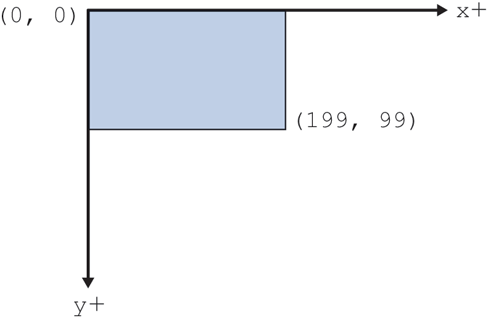
\includegraphics[width=\maxwidth,height=\maxheight,width=0.9\linewidth]{Figures/img_p136_1.png}
\end{center}

Điều này ban đầu có thể gây nhầm lẫn, vì bạn có thể đã quen với các hệ
tọa độ trong đó các giá trị \(y\) giảm dần khi bạn di chuyển xuống dưới.
Tuy nhiên, bạn sẽ sớm quen với nó thôi.

\subsection{Vẽ các đường và hình dạng (Drawing Lines and
Shapes)}\label{vux1ebd-cuxe1c-ux111ux1b0ux1eddng-vuxe0-huxecnh-dux1ea1ng-drawing-lines-and-shapes}

Vậy làm thế nào để bạn thực sự vẽ một cái gì đó? Để vẽ các hình dạng và
các đường thẳng, bạn không nói chuyện trực tiếp với
\texttt{DrawingPanel}, mà nói với một đối tượng liên quan có kiểu
\texttt{Graphics}. Hãy coi \texttt{DrawingPanel} như một bức tranh
canvas và đối tượng \texttt{Graphics} như một cây cọ vẽ. Lớp
\texttt{DrawingPanel} có một phương thức được gọi là
\texttt{getGraphics} để trả về đối tượng \texttt{Graphics} của nó:

\begin{verbatim}
Graphics g = panel.getGraphics();
\end{verbatim}

Một trong những lệnh vẽ đơn giản nhất là \texttt{drawLine}, nhận bốn đối
số số nguyên. Ví dụ, lời gọi phương thức:

\begin{verbatim}
g.drawLine(x1, y1, x2, y2);
\end{verbatim}

vẽ một đường thẳng từ điểm \((x_1, y_1)\) đến điểm \((x_2, y_2)\).
Phương thức \texttt{drawLine} chỉ là một trong nhiều lệnh mà một đối
tượng \texttt{Graphics} hiểu được; xem Bảng 3G.2 cho các lệnh khác. Đối
tượng \texttt{Graphics} có nhiều phương thức hơn ngoài các phương thức
được thảo luận ở đây. Bạn có thể đọc về chúng trong tài liệu Java API.

Bảng 3G.2 Một số phương thức hữu ích của đối tượng \texttt{Graphics}

\begin{center}

\includegraphics[width=\maxwidth,height=\maxheight,width=0.9\linewidth]{Figures/img_p138_0.png}
\end{center}

Dưới đây là một chương trình mẫu kết hợp những mảnh ghép này lại với
nhau:

\begin{verbatim}
 1  // Draws a line onto a DrawingPanel.
 2
 3  import java.awt.*;   // for graphics
 4
 5  public class DrawLine1 {
 6      public static void main(String[] args) {
 7          // create the drawing panel
 8          DrawingPanel panel = new DrawingPanel(200, 100);
 9
10          // draw a line on the panel using
11          // the Graphics paintbrush
12          Graphics g = panel.getGraphics();
13          g.drawLine(25, 75, 175, 25);
14      }
15  }
\end{verbatim}

Khi bạn chạy chương trình này, cửa sổ được hiển thị trong Hình 3G.2 sẽ
xuất hiện. Mặc dù nó không phải là văn bản trên giao diện điều khiển như
ở các chương trước, chúng sửa vẫn sẽ gọi đây là ``đầu ra'' của chương
trình.

Hình 3G.2 Đầu ra của \texttt{DrawLine1}

\begin{center}
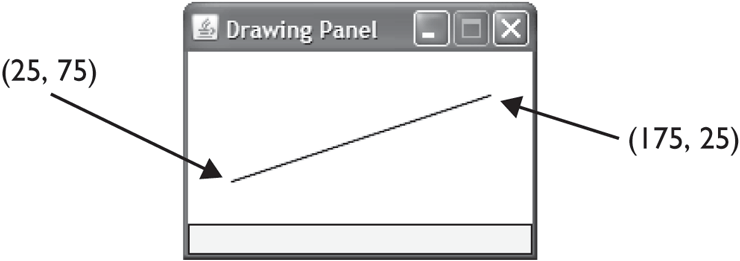
\includegraphics[width=\maxwidth,height=\maxheight,width=0.9\linewidth]{Figures/img_p139_0.png}
\end{center}

(Java có thể được chạy trên nhiều hệ thống khác nhau. Tùy thuộc vào hệ
điều hành của bạn, đầu ra của bạn có thể hơi khác so với các ảnh chụp
màn hình trong chương này.)

Câu lệnh đầu tiên trong \texttt{main} khởi tạo một \texttt{DrawingPanel}
với chiều rộng là 200 và chiều cao là 100. Khi nó đã được khởi tạo, cửa
sổ sẽ bật lên trên màn hình. Câu lệnh thứ hai vẽ một đường thẳng từ
\texttt{(25,\ 75)} đến \texttt{(175,\ 25)}. Điểm đầu tiên nằm ở phần
dưới bên trái của cửa sổ (25 điểm dịch từ bên trái, 75 điểm dịch từ trên
xuống). Điểm thứ hai nằm ở góc trên bên phải (175 điểm dịch từ bên trái,
25 điểm dịch từ trên xuống).

Hãy chú ý đến các dòng mã cụ thể này:

\begin{verbatim}
Graphics g = panel.getGraphics();
g.drawLine(25, 75, 175, 25);
\end{verbatim}

Bạn có thể tự hỏi tại sao bạn không thể nói đơn giản là:

\begin{verbatim}
panel.drawLine(25, 75, 175, 25);   // this is illegal
\end{verbatim}

Vấn đề là có hai đối tượng khác nhau tham gia vào chương trình này: bản
thân \texttt{DrawingPanel} (bức tranh canvas) và đối tượng
\texttt{Graphics} liên kết với panel (cây cọ vẽ). Panel không biết cách
vẽ một đường thẳng; chỉ có đối tượng \texttt{Graphics} mới biết cách
thực hiện việc này. Bạn phải cẩn thận để đảm bảo rằng bạn đang nói
chuyện với đúng đối tượng khi bạn đưa ra một lệnh.

Yêu cầu này có thể gây nhầm lẫn, nhưng nó rất phổ biến trong các chương
trình Java. Trên thực tế, trong một chương trình Java điển hình, có hàng
trăm (nếu không muốn nói là hàng nghìn) đối tượng tương tác với nhau.
Những tương tác này không khác nhiều so với tương tác giữa con người với
nhau. Nếu bạn muốn lên lịch một cuộc họp, một giám đốc điều hành bận rộn
của công ty có thể nói với bạn, ``Hãy nói chuyện với thư ký của tôi về
điều đó.'' Hoặc nếu bạn đang hỏi những câu hỏi pháp lý khó, một người có
thể nói với bạn, ``Hãy nói chuyện với luật sư của tôi về điều đó.''
Trong trường hợp này, \texttt{DrawingPanel} không biết cách vẽ, vì vậy
nếu nó có thể nói, nó sẽ nói, ``Hãy nói chuyện với đối tượng
\texttt{Graphics} của tôi về điều đó.''

Sử dụng đối tượng \texttt{Graphics} mà không lưu trữ nó trong một biến
cũng hợp lệ, như thế này:

\begin{verbatim}
panel.getGraphics().drawLine(25, 75, 175, 25);    // also legal
\end{verbatim}

Nhưng bạn sẽ thường muốn gửi một số lệnh đến đối tượng
\texttt{Graphics}, vì vậy sẽ thuận tiện hơn khi đặt tên cho nó và lưu
trữ nó trong một biến.

Hãy xem một ví dụ phức tạp hơn:

\begin{verbatim}
 1  // Draws three lines to make a triangle.
 2
 3  import java.awt.*;
 4
 5  public class DrawLine2 {
 6      public static void main(String[] args) {
 7          DrawingPanel panel = new DrawingPanel(200, 100);
 8
 9          // draw a triangle on the panel
10          Graphics g = panel.getGraphics();
11          g.drawLine(25, 75, 100, 25);
12          g.drawLine(100, 25, 175, 75);
13          g.drawLine(25, 75, 175, 75);
14      }
15  }
\end{verbatim}

Chương trình này vẽ ba đường thẳng khác nhau để tạo thành một hình tam
giác, như được hiển thị trong Hình 3G.3. Các đường thẳng được vẽ giữa ba
điểm khác nhau. Ở góc dưới bên trái, chúng ta có điểm
\texttt{(25,\ 75)}. Ở giữa phía trên, chúng ta có điểm
\texttt{(100,\ 25)}. Và ở góc dưới bên phải, chúng ta có điểm
\texttt{(175,\ 75)}. Các lời gọi khác nhau trên \texttt{drawLine} chỉ
đơn giản là vẽ các đường thẳng nối ba điểm này lại.

Hình 3G.3 Đầu ra của \texttt{DrawLine2}

\begin{center}
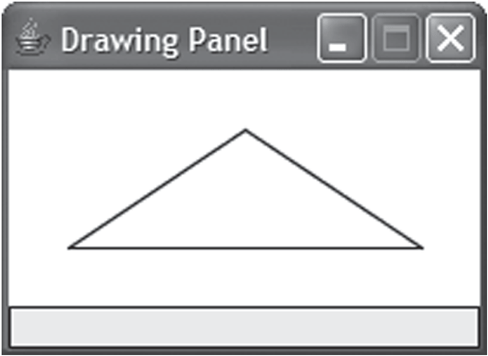
\includegraphics[width=\maxwidth,height=\maxheight,width=0.9\linewidth]{Figures/img_p142_0.png}
\end{center}

Đối tượng \texttt{Graphics} cũng có các phương thức để vẽ các hình dạng
cụ thể. Ví dụ, bạn có thể vẽ các hình chữ nhật với phương thức
\texttt{drawRect}:

\begin{verbatim}
g.drawRect(x, y, width, height);
\end{verbatim}

Câu lệnh này vẽ một hình chữ nhật có tọa độ góc trên bên trái là
\((x, y)\) và chiều cao cùng chiều rộng cho trước.

Một hình dạng khác mà bạn thường muốn vẽ là một hình tròn hoặc, tổng
quát hơn là một hình bầu dục (oval). Nhưng làm thế nào để bạn xác định
nó xuất hiện ở đâu và nó lớn đến mức nào?

Điều bạn thực sự chỉ định là cái được gọi là ``bounding rectangle''
(hình chữ nhật giới hạn) của hình tròn hoặc hình bầu dục. Java sẽ vẽ
hình bầu dục lớn nhất có thể nằm gọn bên trong hình chữ nhật đó. Vì vậy,
lời gọi phương thức:

\begin{verbatim}
g.drawOval(x, y, width, height);
\end{verbatim}

sẽ vẽ hình bầu dục lớn nhất vừa với hình chữ nhật có tọa độ góc trên bên
trái \((x, y)\) và chiều cao cùng chiều rộng cho trước.

Chú ý rằng hai giá trị đầu tiên được truyền vào \texttt{drawRect} và
\texttt{drawOval} là các tọa độ, trong khi hai giá trị tiếp theo là
chiều rộng và chiều cao. Ví dụ, đây là một chương trình ngắn vẽ hai hình
chữ nhật và hai hình bầu dục:

\begin{verbatim}
 1  // Draws several shapes.
 2
 3  import java.awt.*;
 4
 5  public class DrawShapes1 {
 6      public static void main(String[] args) {
 7          DrawingPanel panel = new DrawingPanel(200, 100);
 8
 9          Graphics g = panel.getGraphics();
10          g.drawRect(25, 50, 20, 20);
11          g.drawRect(150, 10, 40, 20);
12          g.drawOval(50, 25, 20, 20);
13          g.drawOval(150, 50, 40, 20);
14      }
15  }
\end{verbatim}

Hình 3G.4 cho thấy đầu ra của chương trình.

Hình 3G.4 Đầu ra của \texttt{DrawShapes1}

\begin{center}

\includegraphics[width=\maxwidth,height=\maxheight,width=0.9\linewidth]{Figures/img_p144_0.png}
\end{center}

Hình chữ nhật đầu tiên có góc trên bên trái của nó ở tọa độ
\texttt{(25,\ 50)}. Chiều rộng và chiều cao của nó đều là 20, vì vậy đây
là một hình vuông. Tọa độ của góc dưới bên phải của nó sẽ là
\texttt{(45,\ 70)}, hay lớn hơn tọa độ \((x, y)\) của góc trên bên trái
20 đơn vị. Chương trình cũng vẽ một hình chữ nhật có góc trên bên trái
tại \texttt{(150,\ 10)} có chiều rộng là 40 và chiều cao là 20 (rộng hơn
cao). Hình chữ nhật giới hạn của hình bầu dục đầu tiên có tọa độ góc
trên bên trái là \texttt{(50,\ 25)} và chiều rộng cũng như chiều cao là
20. Nói cách khác, nó là một hình tròn.

Hình chữ nhật giới hạn của hình bầu dục thứ hai có tọa độ góc trên bên
trái là \texttt{(150,\ 50)}, chiều rộng là 40, và chiều cao là 20 (nó là
một hình bầu dục rộng hơn là cao).

Đôi khi bạn không chỉ muốn vẽ đường viền (outline) của một hình dạng;
bạn muốn tô màu (paint) toàn bộ khu vực bằng một màu cụ thể. Có các biến
thể của các phương thức \texttt{drawRect} và \texttt{drawOval} được gọi
là \texttt{fillRect} và \texttt{fillOval} thực hiện chính xác điều đó,
vẽ một hình chữ nhật hoặc hình bầu dục và tô màu nó bằng màu sơn hiện
tại (mặc định là màu đen). Hãy thay đổi hai trong số các lời gọi trong
chương trình trước thành các thao tác ``tô màu'' (fill) thay vì các thao
tác ``vẽ'' (draw):

\begin{verbatim}
 1  // Draws and fills several shapes.
 2
 3  import java.awt.*;
 4
 5  public class DrawShapes2 {
 6      public static void main(String[] args) {
 7          DrawingPanel panel = new DrawingPanel(200, 100);
 8
 9          Graphics g = panel.getGraphics();
10          g.fillRect(25, 50, 20, 20);
11          g.drawRect(150, 10, 40, 20);
12          g.drawOval(50, 25, 20, 20);
13          g.fillOval(150, 50, 40, 20);
14      }
15  }
\end{verbatim}

Bây giờ chúng ta sẽ nhận được đầu ra được hiển thị trong Hình 3G.5 thay
thế.

Hình 3G.5 Đầu ra của \texttt{DrawShapes2}

\begin{center}
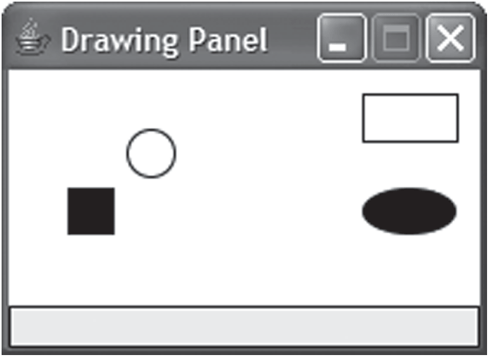
\includegraphics[width=\maxwidth,height=\maxheight,width=0.9\linewidth]{Figures/img_p146_1.png}
\end{center}

\subsection{Màu sắc (Colors)}\label{muxe0u-sux1eafc-colors}

Tất cả các hình dạng và đường thẳng được vẽ bởi các chương trình trước
đều có màu đen, và tất cả các panel đều có nền màu trắng. Đây là các màu
mặc định, nhưng bạn có thể thay đổi màu nền của panel, và bạn có thể
thay đổi màu được sử dụng bởi đối tượng \texttt{Graphics} bao nhiêu lần
tùy thích. Để thay đổi các màu này, bạn sử dụng lớp \texttt{Color} tiêu
chuẩn, là một phần của gói \texttt{java.awt}.

Có một số màu được định nghĩa sẵn mà bạn có thể tham chiếu trực tiếp.
Chúng được định nghĩa dưới dạng các hằng số lớp (class constants) trong
lớp \texttt{Color} (giống như nhiều hằng số chúng ta đã sử dụng trong
Chương 2). Tên của các hằng số này đều được viết hoa và mang tính tự
giải thích. Để tham chiếu đến một trong những màu này, bạn phải đặt
trước nó bằng tên lớp và dấu chấm, như \texttt{Color.GREEN} hoặc
\texttt{Color.BLUE}. Các hằng số \texttt{Color} được định nghĩa sẵn được
liệt kê trong Bảng 3G.3.

Bảng 3G.3 Các hằng số Màu (Color Constants)

\begin{center}

\includegraphics[width=\maxwidth,height=\maxheight,width=0.9\linewidth]{Figures/img_p147_0.png}
\end{center}

Như đã đề cập trước đó, đối tượng \texttt{DrawingPanel} có một phương
thức có thể được sử dụng để thay đổi màu nền bao phủ toàn bộ panel:

\begin{verbatim}
panel.setBackground(Color.YELLOW);
\end{verbatim}

Tương tự, đối tượng \texttt{Graphics} có một phương thức có thể được sử
dụng để thay đổi màu hiện tại dùng để vẽ hoặc tô màu các hình dạng và
đường thẳng:

\begin{verbatim}
g.setColor(Color.MAGENTA);
\end{verbatim}

Việc gọi \texttt{setColor} giống như nhúng cây cọ vẽ của bạn vào một màu
sơn khác. Từ thời điểm đó trở đi, tất cả các thao tác vẽ và tô màu sẽ
được thực hiện bằng màu đã chỉ định. Ví dụ, dưới đây là một phiên bản
khác của chương trình trước đó sử dụng màu nền lục lam (cyan - xanh
nhạt) và tô màu hình bầu dục và hình vuông bằng màu trắng thay vì màu
đen:

\begin{verbatim}
 1  // Draws and fills shapes in different colors.
 2
 3  import java.awt.*;
 4
 5  public class DrawColoredShapes {
 6      public static void main(String[] args) {
 7          DrawingPanel panel = new DrawingPanel(200, 100);
 8          panel.setBackground(Color.CYAN);
 9
10          Graphics g = panel.getGraphics();
11          g.drawRect(150, 10, 40, 20);
12          g.drawOval(50, 25, 20, 20);
13          g.setColor(Color.WHITE);
14          g.fillOval(150, 50, 40, 20);
15          g.fillRect(25, 50, 20, 20);
16      }
17  }
\end{verbatim}

Chương trình này tạo ra đầu ra được hiển thị trong Hình 3G.6. (Các hình
ảnh được hiển thị trong cuốn sách giáo khoa này có thể không khớp với
các màu bạn sẽ thấy trên màn hình của mình.)

Hình 3G.6 Đầu ra của \texttt{DrawColoredShapes}

\begin{center}

\includegraphics[width=\maxwidth,height=\maxheight,width=0.9\linewidth]{Figures/img_p148_0.png}
\end{center}

Lưu ý rằng bạn yêu cầu panel thiết lập màu nền (background color), trong
khi bạn yêu cầu đối tượng \texttt{Graphics} thiết lập màu tiền cảnh
(foreground color). Lý do là màu nền là một thuộc tính của toàn bộ cửa
sổ, trong khi màu tiền cảnh chỉ ảnh hưởng đến các hình dạng cụ thể mà
bạn vẽ.

Lưu ý thêm rằng thứ tự của các lời gọi đã được sắp xếp lại. Hai lệnh vẽ
xuất hiện trước, sau đó là lời gọi trên \texttt{setColor} để thay đổi
màu thành màu trắng, rồi đến hai lệnh tô màu. Điều này đảm bảo rằng thao
tác vẽ được thực hiện bằng màu đen và thao tác tô màu được thực hiện
bằng màu trắng. Thứ tự các phép toán rất quan trọng trong các chương
trình vẽ này, do đó bạn sẽ phải theo dõi xem màu hiện tại của mình là gì
mỗi khi bạn đưa ra lệnh mới để vẽ hoặc tô màu một cái gì đó.

\begin{center}
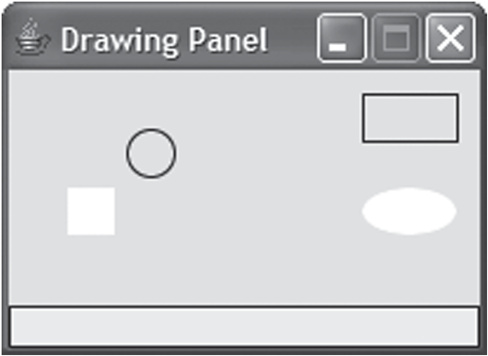
\includegraphics[width=\maxwidth,height=\maxheight,width=0.9\linewidth]{Figures/img_p149_0.png}
\end{center}

\begin{quote}
{[}!WARNING{]} LỖI LẬP TRÌNH PHỔ BIẾN \textbf{Hiểu lầm về Draw so với
Fill}

Một số lập trình viên mới nghĩ rằng một hình dạng phải được vẽ (chẳng
hạn như với \texttt{drawRect}) trước khi nó có thể được tô màu (chẳng
hạn như với \texttt{fillRect}). Điều này không đúng. Trên thực tế, khi
bạn đang cố gắng vẽ một hình dạng có đường viền (outlined shape), đây
chính xác là điều sai lầm. Giả sử bạn muốn vẽ một hình chữ nhật màu xanh
lá cây kích thước \(60 \times 30\) với viền đen tại tọa độ
\texttt{(20,\ 50)}. Bạn có thể viết mã sau:

\begin{verbatim}
g.setColor(Color.BLACK);   // incorrect code
g.drawRect(20, 50, 60, 30);
g.setColor(Color.GREEN);
g.fillRect(20, 50, 60, 30);
\end{verbatim}

Tuy nhiên, lệnh \texttt{fill} bao phủ các pixel giống hệt như lệnh
\texttt{draw}, và phần bên trong màu xanh lá cây sẽ được vẽ đè lên đường
viền màu đen, dẫn đến diện mạo sau:

\begin{center}
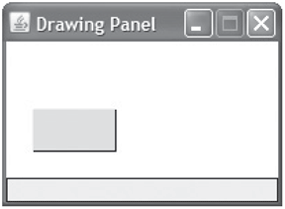
\includegraphics[width=\maxwidth,height=\maxheight,width=0.9\linewidth]{Figures/img_p151_0.png}
\end{center}

Thay vào đó, mã nên tô màu phần bên trong của hình chữ nhật trước, sau
đó mới vẽ đường viền màu đen, để đảm bảo rằng đường viền hiển thị nằm
trên phần tô màu. Dưới đây là đoạn mã chính xác và đầu ra của nó:

\begin{verbatim}
g.setColor(Color.GREEN);   // corrected code
g.fillRect(20, 50, 60, 30);
g.setColor(Color.BLACK);
g.drawRect(20, 50, 60, 30);
\end{verbatim}

\begin{center}
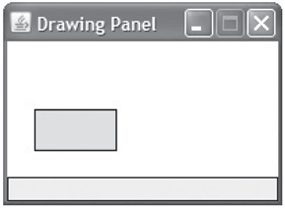
\includegraphics[width=\maxwidth,height=\maxheight,width=0.9\linewidth]{Figures/img_p151_1.png}
\end{center}
\end{quote}

\subsection{Vẽ bằng các vòng lặp (Drawing with
Loops)}\label{vux1ebd-bux1eb1ng-cuxe1c-vuxf2ng-lux1eb7p-drawing-with-loops}

Trong mỗi ví dụ trước, chúng ta đã sử dụng các hằng số đơn giản cho các
lệnh vẽ và tô màu, nhưng có thể sử dụng các biểu thức (expressions). Ví
dụ, giả sử chúng ta bám sát kích thước \texttt{DrawingPanel} của mình là
rộng 200 pixel và cao 100 pixel và chúng ta muốn tạo ra một chuỗi bốn
hình chữ nhật nằm chéo kéo dài từ góc trên bên trái đến góc dưới bên
phải, mỗi hình chứa một hình bầu dục màu trắng bên trong. Nói cách khác,
chúng ta muốn tạo ra đầu ra được hiển thị trong Hình 3G.7.

Hình 3G.7 Đầu ra mong muốn của \texttt{DrawLoop1}

\begin{center}
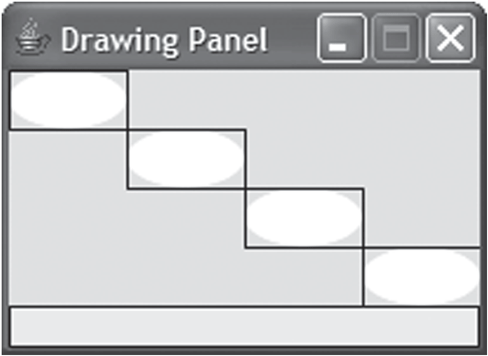
\includegraphics[width=\maxwidth,height=\maxheight,width=0.9\linewidth]{Figures/img_p152_1.png}
\end{center}

Chiều rộng tổng thể 200 và chiều cao tổng thể 100 được chia đều thành
bốn hình chữ nhật, có nghĩa là tất cả chúng đều phải rộng 50 pixel và
cao 25 pixel. Vì vậy, giá trị chiều rộng và chiều cao cho cả bốn hình
chữ nhật là giống nhau, nhưng vị trí góc trên bên trái của chúng thì
khác nhau. Góc trên bên trái của hình chữ nhật đầu tiên là ở
\texttt{(0,\ 0)}, cái thứ hai là ở \texttt{(50,\ 25)}, cái thứ ba là ở
\texttt{(100,\ 50)} và cái thứ tư là ở \texttt{(150,\ 75)}. Chúng ta cần
viết mã để tạo ra các tọa độ khác nhau này.

\begin{center}

\includegraphics[width=\maxwidth,height=\maxheight,width=0.9\linewidth]{Figures/img_p153_0.png}
\end{center}

Đây là một nơi tuyệt vời để sử dụng vòng lặp \texttt{for}. Sử dụng các
kỹ thuật được giới thiệu trong Chương 2, chúng ta có thể lập một bảng và
phát triển một công thức cho các tọa độ. Trong trường hợp này, sẽ dễ
dàng hơn nếu vòng lặp bắt đầu bằng \texttt{0} thay vì \texttt{1}, điều
này thường xảy ra với các chương trình vẽ. Dưới đây là một chương trình
tạo ra nỗ lực đầu tiên tốt để tạo ra đầu ra mong muốn:

\begin{verbatim}
 1  // Draws boxed ovals using a for loop (flawed version).
 2
 3  import java.awt.*;
 4
 5  public class DrawLoop1 {
 6      public static void main(String[] args) {
 7          DrawingPanel panel = new DrawingPanel(200, 100);
 8          panel.setBackground(Color.CYAN);
 9
10          Graphics g = panel.getGraphics();
11          for (int i = 0; i < 4; i++) {
12              g.drawRect(i * 50, i * 25, 50, 25);
13              g.setColor(Color.WHITE);
14              g.fillOval(i * 50, i * 25, 50, 25);
15          }
16      }
17  }
\end{verbatim}

Chương trình này tạo ra đầu ra được hiển thị trong Hình 3G.8.

Hình 3G.8 Đầu ra của \texttt{DrawLoop1}

\begin{center}
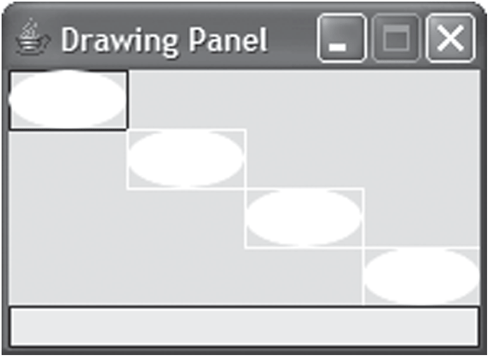
\includegraphics[width=\maxwidth,height=\maxheight,width=0.9\linewidth]{Figures/img_p154_1.png}
\end{center}

Tọa độ và kích thước đã đúng, nhưng màu sắc thì không. Thay vì có được
bốn hình chữ nhật màu đen có hình bầu dục màu trắng bên trong, chúng ta
lại có một hình chữ nhật màu đen và ba hình chữ nhật màu trắng. Đó là vì
chúng ta chỉ có một lời gọi \texttt{setColor} bên trong vòng lặp. Ban
đầu màu sắc sẽ

được đặt thành màu đen, đó là lý do tại sao hình chữ nhật đầu tiên xuất
hiện màu đen. Nhưng khi chúng ta gọi \texttt{setColor} thay đổi màu
thành màu trắng, mọi lệnh vẽ và tô màu tiếp theo đều được thực hiện bằng
màu trắng, bao gồm cả hình chữ nhật thứ hai, thứ ba và thứ tư.

Vì vậy, chúng ta cần bao gồm các lời gọi để đặt màu thành màu đen, để vẽ
các hình chữ nhật và đặt màu thành màu trắng để vẽ các hình bầu dục được
tô màu. Đồng thời, tốt nhất là nên đổi thứ tự các tác vụ này. Các hình
chữ nhật và hình bầu dục chồng lên nhau một chút, và chúng ta muốn hình
chữ nhật được vẽ đè lên hình bầu dục hơn là ngược lại. Chương trình sau
đây tạo ra đầu ra chính xác:

\begin{verbatim}
 1  // Draws boxed ovals using a for loop.
 2
 3  import java.awt.*;
 4
 5  public class DrawLoop2 {
 6      public static void main(String[] args) {
 7          DrawingPanel panel = new DrawingPanel(200, 100);
 8          panel.setBackground(Color.CYAN);
 9
10          Graphics g = panel.getGraphics();
11          for (int i = 0; i < 4; i++) {
12              g.setColor(Color.WHITE);
13              g.fillOval(i * 50, i * 25, 50, 25);
14              g.setColor(Color.BLACK);
15              g.drawRect(i * 50, i * 25, 50, 25);
16          }
17      }
18  }
\end{verbatim}

Cũng có thể tự tạo các đối tượng \texttt{Color} tùy chỉnh, thay vì sử
dụng các màu hằng số được cung cấp trong lớp \texttt{Color}. Màn hình
máy tính sử dụng đỏ, xanh lá cây và xanh dương (RGB) làm các màu cơ bản,
vì vậy khi bạn khởi tạo một đối tượng \texttt{Color}, bạn sẽ truyền các
giá trị tham số của riêng mình cho độ đỏ (redness), độ xanh lá cây
(greenness) và độ xanh dương (blueness) của màu sắc:

\begin{verbatim}
new Color(red, green, blue)
\end{verbatim}

Các thành phần đỏ/xanh lá cây/xanh dương phải là các giá trị số nguyên
từ \texttt{0} đến \texttt{255}. Giá trị càng cao, thì càng có nhiều màu
đó được trộn vào. Tất cả giá trị \texttt{0} tạo ra màu đen, và tất cả
giá trị \texttt{255} tạo ra màu trắng. Các giá trị
\texttt{(0,\ 255,\ 0)} tạo ra một màu xanh lá cây thuần túy, trong khi
các giá trị \texttt{(128,\ 0,\ 128)} tạo ra một màu tím đậm (bởi vì màu
đỏ và màu xanh dương được pha trộn). Hãy tìm kiếm ``RGB table'' trên
công cụ tìm kiếm yêu thích của bạn để tìm bảng các màu thông dụng.

Chương trình sau minh họa việc sử dụng các màu tùy chỉnh. Nó sử dụng một
hằng số lớp cho số lượng hình chữ nhật để vẽ và tạo ra một sự pha trộn
(blend) màu sắc từ đen sang trắng:

\begin{verbatim}
 1  // Draws a smooth color gradient from black to white.
 2
 3  import java.awt.*;
 4
 5  public class DrawColorGradient {
 6      public static final int RECTS = 32;
 7
 8      public static void main(String[] args) {
 9          DrawingPanel panel = new DrawingPanel(256, 256);
10          panel.setBackground(new Color(255, 128, 0)); // orange
11
12          Graphics g = panel.getGraphics();
13
14          // from black to white, top left to bottom right
15          for (int i = 0; i < RECTS; i++) {
16              int shift = i * 256 / RECTS;
17              g.setColor(new Color(shift, shift, shift));
18              g.fillRect(shift, shift, 20, 20);
19          }
20      }
21  }
\end{verbatim}

Chương trình này tạo ra đầu ra được hiển thị trong Hình 3G.9.

Hình 3G.9 Đầu ra của \texttt{DrawColorGradient}

\begin{center}

\includegraphics[width=\maxwidth,height=\maxheight,width=0.9\linewidth]{Figures/img_p157_0.png}
\end{center}

Lưu trữ một đối tượng \texttt{Color} vào một biến hoặc truyền nó như một
tham số cũng là hợp lệ. Ví dụ, chúng ta có thể viết mã tô màu trong
chương trình trước như sau:

\begin{verbatim}
Color c = new Color(shift, shift, shift);
g.setColor(c);
...
\end{verbatim}

\begin{center}
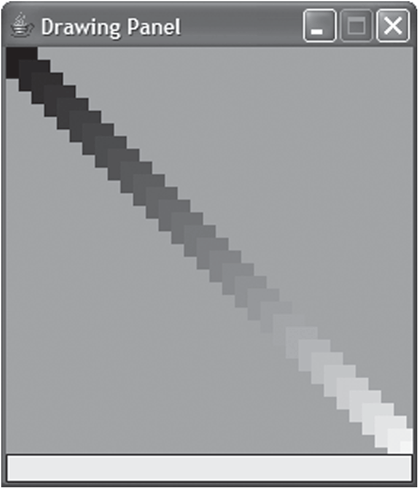
\includegraphics[width=\maxwidth,height=\maxheight,width=0.9\linewidth]{Figures/img_p158_0.png}
\end{center}

Chúng ta sẽ sử dụng ý tưởng này sau khi tham số hóa (parameterizing) màu
sắc trong Nghiên cứu điển hình (Case Study) của chương này.

\subsection{Văn bản và Phông chữ (Text and
Fonts)}\label{vux103n-bux1ea3n-vuxe0-phuxf4ng-chux1eef-text-and-fonts}

Một lệnh vẽ khác đáng được nhắc đến có thể được sử dụng để đưa văn bản
vào các bức vẽ của bạn. Phương thức \texttt{drawString} của đối tượng
\texttt{Graphics} sẽ vẽ một đối tượng \texttt{String} được cung cấp với
góc dưới bên trái của nó ở tọa độ \((x, y)\):

\begin{verbatim}
g.drawString(message, x, y);
\end{verbatim}

Quy ước này hơi khác một chút so với quy ước chúng ta đã sử dụng cho
\texttt{drawRect}. Với \texttt{drawRect}, chúng ta đã chỉ định các tọa
độ của góc trên bên trái. Ở đây, chúng ta chỉ định các tọa độ của góc
dưới bên trái. Theo mặc định, văn bản được vẽ với chiều cao xấp xỉ 10
pixel. Dưới đây là một chương trình mẫu sử dụng một vòng lặp để vẽ một
đối tượng \texttt{String} cụ thể 10 lần khác nhau, mỗi lần thụt lề 5
pixel sang bên phải và di chuyển xuống 10 pixel từ trên cùng:

\begin{verbatim}
 1  // Draws a message several times.
 2
 3  import java.awt.*;
 4
\end{verbatim}

\begin{verbatim}
 5  public class DrawStringMessage1 {
 6      public static void main(String[] args) {
 7          DrawingPanel panel = new DrawingPanel(200, 100);
 8          panel.setBackground(Color.YELLOW);
 9
10          Graphics g = panel.getGraphics();
11          for (int i = 0; i < 10; i++) {
12              g.drawString("There is no place like home",
13                          i * 5, 10 + i * 10);
14          }
15      }
16  }
\end{verbatim}

Chương trình này tạo ra đầu ra được hiển thị trong Hình 3G.10.

Hình 3G.10 Đầu ra của \texttt{DrawStringMessage}

\begin{center}
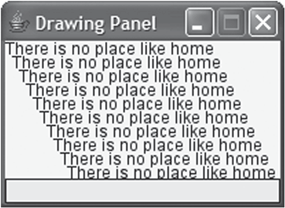
\includegraphics[width=\maxwidth,height=\maxheight,width=0.9\linewidth]{Figures/img_p160_1.png}
\end{center}

Phông chữ (fonts) được sử dụng để mô tả các kiểu dáng (styles) khác nhau
để viết các ký tự trên màn hình. Nếu bạn muốn thay đổi kiểu hoặc kích
thước của văn bản trên màn hình, bạn có thể sử dụng phương thức
\texttt{setFont} của đối tượng \texttt{Graphics}.

\textbf{Phông chữ (Font)} Một thiết kế tổng thể cho một tập hợp các ký
tự văn bản, bao gồm kiểu, kích thước, độ đậm (weight) và diện mạo của
từng ký tự.

Phương thức này thay đổi kích thước và kiểu văn bản mà các chuỗi được
vẽ.

Tham số truyền vào \texttt{setFont} là một đối tượng \texttt{Font}. Một
đối tượng \texttt{Font} được tạo ra bằng cách truyền vào ba tham
số---tên của phông chữ dưới dạng \texttt{String}, kiểu của nó (chẳng hạn
như in đậm hoặc in nghiêng), và kích thước của nó dưới dạng số nguyên:

\begin{verbatim}
new Font(name, style, size)
\end{verbatim}

Các kiểu phông chữ phổ biến như in đậm (bold) được triển khai dưới dạng
các hằng số trong lớp \texttt{Font}. Các hằng số có sẵn và một số tên
phông chữ phổ biến được liệt kê trong các Bảng 3G.4 và 3G.5.

Bảng 3G.4 Các hằng số hữu ích của lớp \texttt{Font}

\begin{center}

\includegraphics[width=\maxwidth,height=\maxheight,width=0.9\linewidth]{Figures/img_p161_0.png}
\end{center}

Bảng 3G.5 Các Tên Phông Chữ Phổ Biến

\begin{center}

\includegraphics[width=\maxwidth,height=\maxheight,width=0.9\linewidth]{Figures/img_p162_0.png}
\end{center}

Giống như trường hợp của màu sắc, việc thiết lập phông chữ chỉ ảnh hưởng
đến các chuỗi được vẽ sau khi phông chữ được thiết lập. Chương trình sau
đây thiết lập một số phông chữ và sử dụng chúng để vẽ các chuỗi:

\begin{verbatim}
 1  // Draws several messages using different fonts.
 2
 3  import java.awt.*;
 4
 5  public class DrawFonts {
 6      public static void main(String[] args) {
 7          DrawingPanel panel = new DrawingPanel(200, 100);
 8          panel.setBackground(Color.PINK);
 9
10          Graphics g = panel.getGraphics();
11          g.setFont(new Font("Monospaced",
12                     Font.BOLD + Font.ITALIC, 36));
13          g.drawString("Too big", 20, 40);
14
15          g.setFont(new Font("SansSerif", Font.PLAIN, 10));
16          g.drawString("Too small", 30, 60);
17
18          g.setFont(new Font("Serif", Font.ITALIC, 18));
19          g.drawString("Just right", 40, 80);
20      }
21  }
\end{verbatim}

Chương trình này tạo ra đầu ra được hiển thị trong Hình 3G.11.

Hình 3G.11 Đầu ra của \texttt{DrawFonts}

\begin{center}
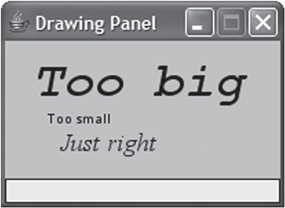
\includegraphics[width=\maxwidth,height=\maxheight,width=0.9\linewidth]{Figures/img_p163_0.png}
\end{center}

\subsection{Hình ảnh (Images)}\label{huxecnh-ux1ea3nh-images}

\texttt{DrawingPanel} cũng có khả năng hiển thị các hình ảnh được tải từ
các tệp ở các định dạng như JPEG, PNG và GIF. Để hiển thị một hình ảnh,
đầu tiên bạn phải tìm một tệp hình ảnh (chẳng hạn như một tệp trên
internet hoặc trên máy tính của bạn) và đặt nó vào cùng thư mục với dự
án mã của bạn. Hình ảnh được hiển thị qua hai bước: đầu tiên, hình ảnh
phải được tải từ ổ cứng vào một đối tượng \texttt{Image}, và sau đó đối
tượng \texttt{Graphics} của panel có thể hiển thị hình ảnh.

\begin{verbatim}
Image img = panel.loadImage("smileyface.png");
g.drawImage(img, x, y, panel);
\end{verbatim}

Các tọa độ \(x\) và \(y\) được truyền vào khi vẽ hình ảnh thể hiện vị
trí pixel ở góc trên cùng/bên trái của nó.

Có một vài điều kỳ quặc đối với cú pháp. Một là chúng ta sử dụng
\texttt{DrawingPanel} để tải hình ảnh, trong khi bạn sử dụng đối tượng
\texttt{Graphics} để vẽ nó. Rất dễ vô tình lẫn lộn hai thứ này. Ngoài
ra, không giống như các lệnh vẽ khác, \texttt{drawImage} yêu cầu bạn
truyền \texttt{DrawingPanel} làm tham số cuối cùng cho phương thức. Điều
này được yêu cầu bởi lớp \texttt{Graphics} của Java để mã có thể biên
dịch.

Ví dụ, chương trình sau đây tải một hình ảnh trông giống như bức vẽ của
một cầu vồng và vẽ nó lên \texttt{DrawingPanel} với một chuỗi văn bản
nằm dưới nó.

\begin{verbatim}
 1  // This program displays a rainbow from an image file.
 2  import java.awt.*;
 3
 4  public class DrawRainbow {
 5      public static void main(String[] args) {
 6          DrawingPanel panel = new DrawingPanel(280, 200);
 7          Image rainbow = panel.loadImage("rainbow.png");
 8          Graphics g = panel.getGraphics();
 9          g.drawImage(rainbow, 0, 0, panel);
10          g.drawString("Somewhere over the rainbow...", 10, 
11 180);
12      }
13  }
\end{verbatim}

Chương trình tạo ra đầu ra được hiển thị trong Hình 3G.12.

\begin{center}

\includegraphics[width=\maxwidth,height=\maxheight,width=0.9\linewidth]{Figures/img_p164_0.png}
\end{center}

Hình 3G.12 Đầu ra của \texttt{DrawRainbow}

Nếu bạn muốn vẽ cùng một hình ảnh nhiều lần trên panel, bạn không cần
phải lặp lại phần \texttt{loadImage} của quá trình này. Việc tải hình
ảnh một lần duy nhất và sau đó vẽ nó bao nhiêu lần tùy thích sẽ hiệu quả
hơn nhiều. Đoạn mã sau đây sẽ vẽ một vài bản sao của một hình ảnh trong
một tệp có tên là \texttt{smiley.png}, có kích thước \(100 \times 100\)
pixel. Đầu ra của đoạn mã này được hiển thị trong Hình 3G.13.

Hình 3G.13 Đầu ra mặt cười

\begin{center}
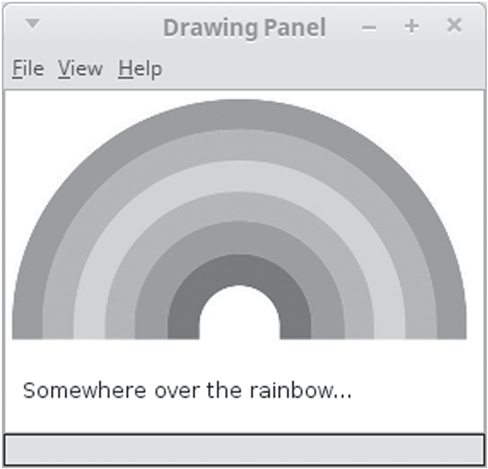
\includegraphics[width=\maxwidth,height=\maxheight,width=0.9\linewidth]{Figures/img_p165_1.png}
\end{center}

\begin{verbatim}
Image smileyFace = panel.loadImage("smiley.png");
Graphics g = panel.getGraphics();
for (int i = 0; i < 4; i++) {
    g.drawImage(smileyFace, i * 110 + 10, 10, panel);
}
\end{verbatim}

\begin{center}
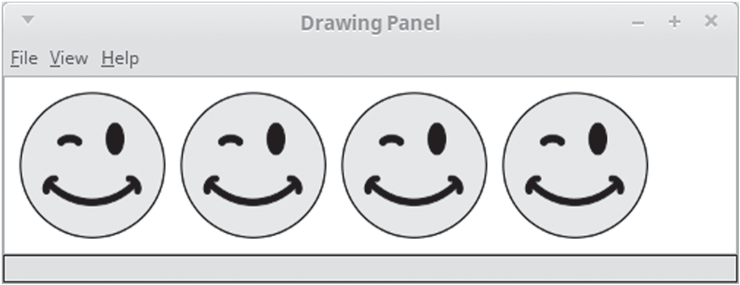
\includegraphics[width=\maxwidth,height=\maxheight,width=0.9\linewidth]{Figures/img_p166_0.png}
\end{center}

\subsection{3G.2 Phân rã thủ tục với Đồ họa (Procedural Decomposition
with
Graphics)}\label{g.2-phuxe2n-ruxe3-thux1ee7-tux1ee5c-vux1edbi-ux111ux1ed3-hux1ecda-procedural-decomposition-with-graphics-1}

Nếu bạn viết các chương trình vẽ phức tạp, bạn sẽ muốn chia nhỏ chúng
thành một số phương thức tĩnh (static methods) để cấu trúc mã và loại bỏ
sự dư thừa. Khi thực hiện việc này, bạn sẽ phải truyền đối tượng
\texttt{Graphics} cho từng phương thức tĩnh mà bạn giới thiệu. Để lấy
một ví dụ nhanh, chương trình \texttt{DrawStringMessage1} từ phần trước
có thể được chia thành một phương thức \texttt{main} và một phương thức
\texttt{drawText}, như sau:

\begin{verbatim}
 1  // Draws a message several times using a static method.
 2
 3  import java.awt.*;
 4
 5  public class DrawStringMessage2 {
 6      public static void main(String[] args) {
 7          DrawingPanel panel = new DrawingPanel(200, 100);
 8          panel.setBackground(Color.YELLOW);
 9
10          Graphics g = panel.getGraphics();
11          drawText(g);
12      }
13
14      public static void drawText(Graphics g) {
15          for (int i = 0; i < 10; i++) {
16              g.drawString("There is no place like home",
17                           i * 5, 10 + i * 10);
18          }
19      }
20  }
\end{verbatim}

Chương trình này tạo ra cùng một đầu ra như chương trình gốc (Hình
3G.10).

Chương trình sẽ không biên dịch được nếu không truyền
\texttt{Graphics\ g} cho phương thức \texttt{drawText}, bởi vì
\texttt{g} là cần thiết để gọi các phương thức vẽ như
\texttt{drawString} và \texttt{fillRect}.

\subsubsection{Một ví dụ lớn hơn: DrawDiamonds (A Larger Example:
DrawDiamonds)}\label{mux1ed9t-vuxed-dux1ee5-lux1edbn-hux1a1n-drawdiamonds-a-larger-example-drawdiamonds}

Bây giờ chúng ta hãy xem xét một tác vụ phức tạp hơn một chút: vẽ hình
thoi (diamond) lớn nhất có thể nằm vừa trong một hộp có kích thước cụ
thể. Hình thoi lớn nhất có thể nằm vừa trong một hộp có kích thước
\(50 \times 50\) được hiển thị trong Hình 3G.14.

Hình 3G.14 Hình thoi (Diamond)

\begin{center}

\includegraphics[width=\maxwidth,height=\maxheight,width=0.9\linewidth]{Figures/img_p168_0.png}
\end{center}

Mã để vẽ một hình thoi như vậy sẽ là:

\begin{verbatim}
g.drawRect(0, 0, 50, 50);
g.drawLine(0, 25, 25, 0);
g.drawLine(25, 0, 50, 25);
g.drawLine(50, 25, 25, 50);
g.drawLine(25, 50, 0, 25);
\end{verbatim}

Bây giờ hãy tưởng tượng rằng chúng ta muốn vẽ ba hình thoi
\(50 \times 50\) như vậy ở các vị trí khác nhau. Chúng ta có thể biến mã
vẽ hình thoi của mình thành một phương thức \texttt{drawDiamond} mà
chúng ta sẽ gọi ba lần. Vì mỗi hình thoi

sẽ ở một vị trí khác nhau, chúng ta có thể truyền các tọa độ \(x\) và
\(y\) dưới dạng các tham số cho phương thức \texttt{drawDiamond} của
mình.

Một hình thoi được bao quanh bởi một hộp có góc trên cùng bên trái tại
vị trí \texttt{(78,\ 22)} được hiển thị trong Hình 3G.15.

Hình 3G.15 Hình thoi tại \texttt{(78,\ 22)}

\begin{center}
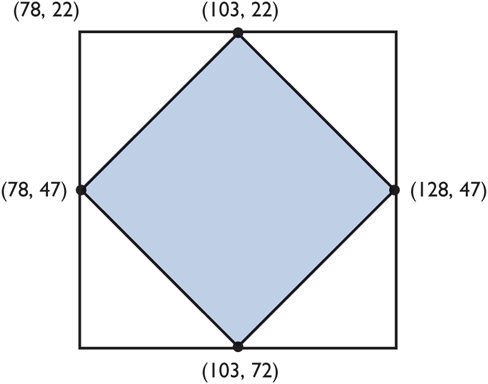
\includegraphics[width=\maxwidth,height=\maxheight,width=0.9\linewidth]{Figures/img_p170_1.png}
\end{center}

Mã để vẽ hình thoi này sẽ là:

\begin{verbatim}
g.drawRect(78, 22, 50, 50);
g.drawLine(78, 47, 103, 22);
g.drawLine(103, 22, 128, 47);
g.drawLine(128, 47, 103, 72);
g.drawLine(103, 72, 78, 47);
\end{verbatim}

Như bạn có thể thấy, các giá trị tham số được truyền cho các phương thức
\texttt{drawRect} và \texttt{drawLine} rất giống với các giá trị của
hình thoi đầu tiên, ngoại trừ việc chúng được dịch chuyển đi 78 theo
hướng \(x\) và 22 theo hướng \(y\) (ngoại trừ tham số thứ ba và thứ tư
của \texttt{drawRect}, vì đây là chiều rộng và chiều cao của hình chữ
nhật). Sự dịch chuyển \texttt{(78,\ 22)} này được gọi là một phần bù
(offset).

Chúng ta có thể tổng quát hóa các tọa độ để truyền vào các lệnh vẽ của
\texttt{Graphics\ g} để chúng hoạt động với bất kỳ hình thoi nào nếu
chúng ta truyền các phần bù \(x\) và \(y\) ở góc trên bên trái của hình
thoi đó. Ví dụ: chúng ta sẽ tổng quát hóa đường thẳng từ
\texttt{(0,\ 25)} trong hình thoi đầu tiên và từ \texttt{(78,\ 47)} đến
\texttt{(103,\ 22)} trong hình thoi thứ hai bằng cách nói rằng đó là một
đường thẳng từ \((x, y + 25)\) đến \((x + 25, y)\), trong đó \((x, y)\)
là phần bù (offset) của hình thoi đã cho.

Chương trình sau đây sử dụng phương thức \texttt{drawDiamond} để vẽ ba
hình thoi mà không bị dư thừa:

\begin{verbatim}
 1  // This program draws several diamond figures of size 50x50.
 2
 3  import java.awt.*;
 4
 5  public class DrawDiamonds {
 6      public static void main(String[] args) {
 7          DrawingPanel panel = new DrawingPanel(250, 150);
 8          Graphics g = panel.getGraphics();
 9
10          drawDiamond(g, 0, 0);
11          drawDiamond(g, 78, 22);
12          drawDiamond(g, 19, 81);
13      }
14
15      // draws a diamond in a 50x50 box
16      public static void drawDiamond(Graphics g, int x, int y) {
17          g.drawRect(x, y, 50, 50);
18          g.drawLine(x, y + 25, x + 25, y);
19          g.drawLine(x + 25, y, x + 50, y + 25);
20          g.drawLine(x + 50, y + 25, x + 25, y + 50);
21          g.drawLine(x + 25, y + 50, x, y + 25);
22      }
23  }
\end{verbatim}

Chương trình này tạo ra đầu ra được hiển thị trong Hình 3G.16.

Hình 3G.16 Đầu ra của \texttt{DrawDiamonds}

\begin{center}

\includegraphics[width=\maxwidth,height=\maxheight,width=0.9\linewidth]{Figures/img_p172_0.png}
\end{center}

Chúng ta có thể vẽ các hình có hoa văn trong các vòng lặp và yêu cầu một
phương thức vẽ gọi một phương thức vẽ khác. Ví dụ: nếu chúng ta muốn vẽ
năm hình thoi, bắt đầu tại tọa độ \texttt{(12,\ 15)} và cách nhau 60
pixel, chúng ta chỉ cần một vòng lặp \texttt{for} lặp lại năm lần và
dịch chuyển tọa độ \(x\) thêm 60 mỗi lần. Đây là một vòng lặp ví dụ:

\begin{verbatim}
for (int i = 0; i < 5; i++) {
    drawDiamond(g, 12 + 60 * i, 15);
}
\end{verbatim}

\begin{center}
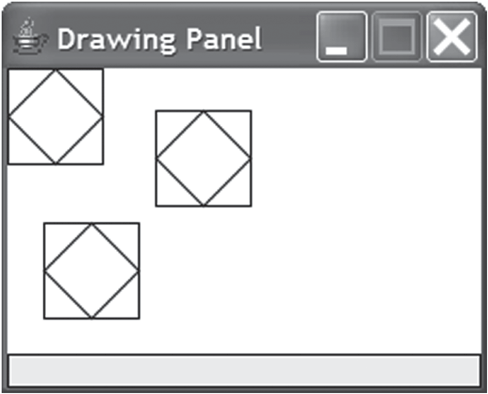
\includegraphics[width=\maxwidth,height=\maxheight,width=0.9\linewidth]{Figures/img_p173_0.png}
\end{center}

Nếu chúng ta tạo một phương thức khác để vẽ đường gồm năm hình thoi,
chúng ta có thể gọi nó từ \texttt{main} để vẽ nhiều đường thẳng chứa các
hình thoi. Dưới đây là phiên bản sửa đổi của chương trình
\texttt{DrawDiamonds} với hai phương thức đồ họa:

\begin{verbatim}
 1  // This program draws several diamond figures of size 50x50.
 2
 3  import java.awt.*;
 4
 5  public class DrawDiamonds2 {
 6      public static void main(String[] args) {
 7          DrawingPanel panel = new DrawingPanel(360, 160);
 8          Graphics g = panel.getGraphics();
 9
10          drawManyDiamonds(g, 12, 15);
11          g.setColor(Color.RED);
12          drawManyDiamonds(g, 55, 100);
13      }
14
15      // draws five diamonds in a horizontal line
16      public static void drawManyDiamonds(Graphics g,
17                                         int x, int y) {
18          for (int i = 0; i < 5; i++) {
19              drawDiamond(g, x + 60 * i, y);
20          }
21      }
22
23      // draws a diamond in a 50x50 box


24      public static void drawDiamond(Graphics g, int x, int y) {
25          g.drawRect(x, y, 50, 50);
26          g.drawLine(x, y + 25, x + 25, y);
27          g.drawLine(x + 25, y, x + 50, y + 25);
28          g.drawLine(x + 50, y + 25, x + 25, y + 50);
29          g.drawLine(x + 25, y + 50, x, y + 25);
30      }
31  }
\end{verbatim}

Chương trình này tạo ra đầu ra được hiển thị trong Hình 3G.17.

Hình 3G.17 Đầu ra của \texttt{DrawDiamonds2}

\begin{center}
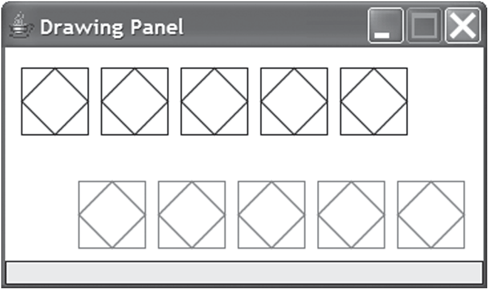
\includegraphics[width=\maxwidth,height=\maxheight,width=0.9\linewidth]{Figures/img_p175_1.png}
\end{center}

\subsection{3G.3 Nghiên cứu điển hình: Kim tự tháp (Case Study:
Pyramids)}\label{g.3-nghiuxean-cux1ee9u-ux111iux1ec3n-huxecnh-kim-tux1ef1-thuxe1p-case-study-pyramids-1}

Hãy tưởng tượng rằng bạn đã được yêu cầu viết một chương trình để vẽ các
hình ảnh trong Hình 3G.18 lên một \texttt{DrawingPanel}.

Hình 3G.18 Đầu ra Kim tự tháp (Pyramids) mong muốn

\begin{center}

\includegraphics[width=\maxwidth,height=\maxheight,width=0.9\linewidth]{Figures/img_p176_1.png}
\end{center}

Bảng vẽ (drawing panel) tổng thể có kích thước là \(350 \times 250\).
Mỗi kim tự tháp cao 100 pixel và rộng 100 pixel. Các kim tự tháp bao gồm
các bậc thang có màu sắc được căn giữa và mở rộng dần về phía dưới, với
các đường viền màu đen xung quanh mỗi bậc thang. Bảng 3G.6 liệt kê các
thuộc tính của từng kim tự tháp.

Bảng 3G.6 Các thuộc tính của Kim tự tháp

\begin{center}
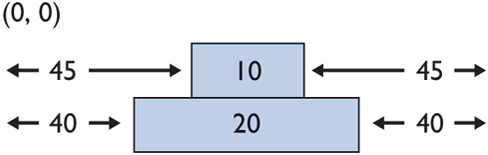
\includegraphics[width=\maxwidth,height=\maxheight,width=0.9\linewidth]{Figures/img_p177_0.png}
\end{center}

\subsubsection{Giải pháp phi cấu trúc một phần (Unstructured Partial
Solution)}\label{giux1ea3i-phuxe1p-phi-cux1ea5u-truxfac-mux1ed9t-phux1ea7n-unstructured-partial-solution}

Khi cố gắng giải quyết một bài toán lớn và phức tạp hơn như bài toán
này, điều quan trọng là phải giải quyết từng phần và cải tiến lặp đi lặp
lại (iterative enhancements) hướng tới một giải pháp hoàn chỉnh. Hãy bắt
đầu bằng cách cố gắng vẽ đúng kim tự tháp màu trắng ở góc trên cùng bên
trái.

Mỗi bậc thang được căn giữa theo chiều ngang trong kim tự tháp. Bậc
thang trên cùng rộng 10 pixel. Do đó, nó được bao quanh bởi \(90/2\)
hoặc 45 pixel khoảng trống ở mỗi bên. Điều đó có nghĩa là góc trên cùng
bên trái của hình chữ nhật \(10 \times 10\) nằm ở tọa độ
\texttt{(45,\ 0)}. Bậc thang thứ hai rộng 20 pixel, có nghĩa là nó được
bao quanh bởi \(80/2\) hoặc 40 pixel ở mỗi bên:

\begin{center}

\includegraphics[width=\maxwidth,height=\maxheight,width=0.9\linewidth]{Figures/img_p177_1.png}
\end{center}

Chương trình sau đây vẽ kim tự tháp màu trắng ở đúng vị trí:

\begin{verbatim}
 1  import java.awt.*;
 2
 3  // Draws the first pyramid only, with a lot of redundancy.
 4  public class Pyramids1 {
 5      public static void main(String[] args) {
 6          DrawingPanel panel = new DrawingPanel(350, 250);
 7          Graphics g = panel.getGraphics();
 8
 9          // draws the border rectangle
10          g.drawRect(0, 0, 100, 100);
11
12          // draws the 10 "stairs" in the white pyramid
13          g.drawRect(45,  0,  10, 10);
14          g.drawRect(40, 10,  20, 10);
15          g.drawRect(35, 20,  30, 10);
16          g.drawRect(30, 30,  40, 10);
17          g.drawRect(25, 40,  50, 10);
18          g.drawRect(20, 50,  60, 10);
19          g.drawRect(15, 60,  70, 10);
20          g.drawRect(10, 70,  80, 10);
21          g.drawRect( 5, 80,  90, 10);
22          g.drawRect( 0, 90, 100, 10);
23      }
24  }
\end{verbatim}

Nhìn vào mã, rõ ràng là có rất nhiều sự dư thừa (redundancy) giữa 10
dòng để vẽ các bậc thang. Kiểm tra các mẫu số trong mỗi cột tiết lộ rằng
giá trị \(x\) giảm đi 5 mỗi lần, giá trị \(y\) tăng thêm 10 mỗi lần,
chiều rộng tăng thêm 10 mỗi lần và chiều cao không đổi.

Một cách khác để mô tả giá trị \(x\) của bậc thang là nói rằng nó bằng
một nửa tổng số 100 trừ đi chiều rộng của bậc thang. Với suy nghĩ đó,
vòng lặp \texttt{for} sau đây vẽ 10 bậc thang mà không có sự lặp lại như
trước đó:

\begin{verbatim}
for (int i = 0; i < 10; i++) {
    int stairWidth = 10 * (i + 1);
    int stairHeight = 10;
    int stairX = (100 - stairWidth) / 2;
    int stairY = 10 * i;
    g.drawRect(stairX, stairY, stairWidth, stairHeight);
}
\end{verbatim}

\subsubsection{Tổng quát hóa việc vẽ các Kim tự tháp (Generalizing the
Drawing of
Pyramids)}\label{tux1ed5ng-quuxe1t-huxf3a-viux1ec7c-vux1ebd-cuxe1c-kim-tux1ef1-thuxe1p-generalizing-the-drawing-of-pyramids}

Tiếp theo, hãy thêm mã để vẽ kim tự tháp (màu đỏ) ở dưới cùng. Vị trí
\((x, y)\) của nó là \texttt{(80,\ 140)} và nó chỉ có năm bậc thang.
Điều đó có nghĩa là mỗi bậc thang

cao và rộng gấp đôi so với các bậc thang trong kim tự tháp màu trắng.

Dựa vào thông tin này, chúng ta có thể xác định rằng góc trên bên trái
của bậc thang trên cùng nằm ở \texttt{(120,\ 140)} và kích thước của nó
là \(20 \times 20\), góc trên bên trái của bậc thang thứ hai nằm ở
\texttt{(110,\ 160)} và kích thước của nó là \(40 \times 20\), và cứ thế
tiếp tục.

Hiện tại, hãy tập trung vào việc lấy đúng tọa độ của các bậc thang và
không lo lắng về màu tô màu đỏ. Dưới đây là một đoạn mã bị dư thừa để vẽ
các bậc thang của kim tự tháp màu đỏ, không có tô màu:

\begin{verbatim}
// draws the border rectangle
g.drawRect(80, 140, 100, 100);
// draws the 5 "stairs" of the red pyramid
g.drawRect(120, 140, 20, 20);
g.drawRect(110, 160, 40, 20);
g.drawRect(100, 180, 60, 20);
g.drawRect( 90, 200, 80, 20);
g.drawRect( 80, 220, 100, 20);
\end{verbatim}

\begin{center}
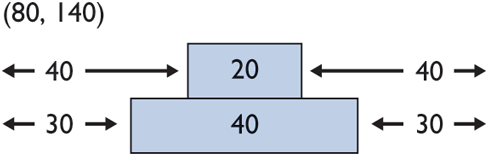
\includegraphics[width=\maxwidth,height=\maxheight,width=0.9\linewidth]{Figures/img_p180_0.png}
\end{center}

Một lần nữa, chúng ta có sự lặp lại giữa năm dòng để vẽ các bậc thang,
vì vậy hãy tìm kiếm một quy luật. Chúng ta sẽ sử dụng một vòng lặp để
loại bỏ sự lặp lại giống như chúng ta đã làm với kim tự tháp trước đó,
nhưng với những sửa đổi thích hợp. Chiều cao của mỗi bậc thang bây giờ
là 20 pixel và chiều rộng của mỗi bậc thang bây giờ là 20 nhân với số
thứ tự của bậc thang đó. Các tọa độ \(x\) và \(y\) khó hơn một chút.
Công thức tính tọa độ \(x\) tương tự như
\texttt{(100\ -\ stairWidth)\ /\ 2} từ trước đó, nhưng lần này nó phải
được dịch sang phải 80 pixel để tính đến vị trí góc trên bên trái của
hộp giới hạn (bounding box). Tọa độ \(y\) tương tự cũng phải được dịch
chuyển xuống dưới 140 pixel. Dưới đây là vòng lặp chính xác:

\begin{verbatim}
// draws the 5 "stairs" of the red pyramid
for (int i = 0; i < 5; i++) {
    int stairWidth = 20 * (i + 1);
    int stairHeight = 20;
    int stairX = 80 + (100 - stairWidth) / 2;
    int stairY = 140 + 20 * i;
    g.drawRect(stairX, stairY, stairWidth, stairHeight);
}
\end{verbatim}

Bạn có thể phát hiện ra quy luật giữa hai vòng lặp \texttt{for} được sử
dụng để vẽ các bậc thang của các kim tự tháp không? Các tọa độ \(x\) và
\(y\) chỉ khác nhau ở việc cộng thêm phần bù (offset) từ
\texttt{(0,\ 0)} trong vòng lặp thứ hai. Chiều rộng và chiều cao của các
bậc thang chỉ khác nhau ở chỗ một bậc thang của kim tự tháp cao 20 pixel
và bậc thang của kim tự tháp kia cao 10 pixel (kết quả của việc lấy tổng
kích thước là 100 chia cho số lượng bậc thang).

Sử dụng thông tin trước đó, hãy biến đoạn mã vẽ kim tự tháp thành một
phương thức mà chúng ta có thể gọi ba lần để tránh sự dư thừa. Các tham
số sẽ là các tọa độ \((x, y)\) của góc trên bên trái của hộp giới hạn
(bounding box) của kim tự tháp và số lượng bậc thang trong kim tự tháp.
Chúng ta cũng sẽ cần truyền \texttt{Graphics\ g} làm tham số để có thể
vẽ lên \texttt{DrawingPanel}. Chúng ta sẽ sửa đổi vòng lặp \texttt{for}
để tính chiều cao của bậc thang trước, sau đó sử dụng chiều cao để tính
chiều rộng của bậc thang và cuối cùng sử dụng chiều rộng và chiều cao để
giúp tính tọa độ \((x, y)\) của bậc thang. Đây là đoạn mã:

\begin{verbatim}
public static void drawPyramid(Graphics g, int x,
                               int y, int stairs) {
    // draws the border rectangle
    g.drawRect(x, y, 100, 100);
    // draws the stairs of the pyramid
    for (int i = 0; i < stairs; i++) {
        int stairHeight = 100 / stairs;
        int stairWidth = stairHeight * (i + 1);
        int stairX = x + (100 - stairWidth) / 2;
        int stairY = y + stairHeight * i;
        g.drawRect(stairX, stairY, stairWidth, stairHeight);
    }
}
\end{verbatim}

Mã trước đó hiện đã được tổng quát hóa để vẽ một kim tự tháp ở bất kỳ vị
trí nào với số lượng bậc thang bất kỳ. Nhưng một yếu tố cuối cùng bị
thiếu: khả năng tạo màu khác nhau cho mỗi kim tự tháp.

\subsubsection{Giải pháp có cấu trúc hoàn chỉnh (Complete Structured
Solution)}\label{giux1ea3i-phuxe1p-cuxf3-cux1ea5u-truxfac-houxe0n-chux1ec9nh-complete-structured-solution}

Đoạn mã trên đúng ngoại trừ việc nó không cho phép chúng ta vẽ các kim
tự tháp với màu sắc thích hợp. Hãy thêm một tham số bổ sung, một đối
tượng \texttt{Color}, vào phương thức của chúng ta và sử dụng nó để tô
màu các bậc thang của kim tự tháp khi cần. Chúng ta sẽ truyền
\texttt{Color.WHITE} làm giá trị của tham số này cho kim tự tháp màu
trắng đầu tiên; nó sẽ tô màu các bậc thang bằng màu trắng, mặc dù điều
này không cần thiết.

Cách để vẽ một hình dạng có màu (filled shape) với một đường viền có màu
khác là tô màu hình dạng đó trước, sau đó sử dụng màu đường viền để vẽ
cùng một hình dạng đó. Ví dụ, để có được các hình chữ nhật màu đỏ có
viền đen, trước tiên chúng ta sẽ sử dụng \texttt{fillRect} với màu đỏ,
sau đó chúng ta sẽ sử dụng \texttt{drawRect} với màu đen cùng với các
tham số tương tự.

Dưới đây là phiên bản mới của phương thức \texttt{drawPyramid} sử dụng
màu tô làm tham số:

\begin{verbatim}
public static void drawPyramid(Graphics g, Color c,
                               int x, int y, int stairs) {
    g.drawRect(x, y, 100, 100);
    for (int i = 0; i < stairs; i++) {
        int stairHeight = 100 / stairs;
        int stairWidth = stairHeight * (i + 1);
        int stairX = x + (100 - stairWidth) / 2;
        int stairY = y + stairHeight * i;
        g.setColor(c);
        g.fillRect(stairX, stairY, stairWidth, stairHeight);
        g.setColor(Color.BLACK);
        g.drawRect(stairX, stairY, stairWidth, stairHeight);
    }
}
\end{verbatim}

Sử dụng phương thức này, giờ đây chúng ta có thể vẽ cả ba kim tự tháp
một cách dễ dàng bằng cách gọi \texttt{drawPyramid} ba lần với các tham
số thích hợp:

\begin{verbatim}
drawPyramid(g, Color.WHITE, 0, 0, 10);
drawPyramid(g, Color.RED, 80, 140, 5);
drawPyramid(g, Color.BLUE, 220, 50, 20);
\end{verbatim}

Một cải tiến cuối cùng mà chúng ta có thể thực hiện cho chương trình
Pyramids của mình là biến kích thước kim tự tháp tổng thể là 100 thành
một hằng số, để không có quá nhiều số 100 nằm rải rác trong mã. Đây là
chương trình hoàn chỉnh:

\begin{verbatim}
 1  // This program draws three colored pyramid figures.
 2
 3  import java.awt.*;
\end{verbatim}

4 5 public class Pyramids \{ 6 public static final int SIZE = 100; 7 8
public static void main(String{[}{]} args) \{ 9 DrawingPanel panel = new
DrawingPanel(350, 250); 10 Graphics g = panel.getGraphics(); 11 12
drawPyramid(g, Color.WHITE, 0, 0, 10); 13 drawPyramid(g, Color.RED, 80,
140, 5); 14 drawPyramid(g, Color.BLUE, 220, 50, 20); 15 \} 16 17 //
draws one pyramid figure with the given 18 // number of stairs at the
given (x, y) position 19 // with the given color 20 public static void
drawPyramid(Graphics g, Color c, 21 int x, int y, int stairs) \{ 22 23
// draws the border rectangle 24 g.drawRect(x, y, SIZE, SIZE); 25 26 //
draws the stairs of the pyramid 27 for (int i = 0; i \textless{} stairs;
i++) \{ 28 int stairHeight = SIZE / stairs; 29 int stairWidth =
stairHeight * (i + 1); 30 int stairX = x + (SIZE - stairWidth) / 2; 31
int stairY = y + stairHeight * i; 32 33 // fills the rectangles with the
fill colors 34 g.setColor(c); 35 g.fillRect(stairX, stairY, stairWidth,
stairHeight); 36 37 // draws the black rectangle outlines 38
g.setColor(Color.BLACK); 39 g.drawRect(stairX, stairY, stairWidth,
stairHeight); 40 \} 41 \} 42 \}

\begin{verbatim}

## Tóm tắt Chương (Chapter Summary)

- `DrawingPanel` là một lớp tùy chỉnh (custom class) được cung cấp bởi các tác giả để dễ dàng hiển thị một cửa sổ đồ họa trên màn hình. Một `DrawingPanel` chứa một đối tượng `Graphics` có thể được sử dụng để vẽ các đường thẳng, văn bản và hình dạng trên màn hình bằng các màu sắc khác nhau.
- Đối tượng `Graphics` có nhiều phương thức hữu ích để vẽ các hình dạng và đường thẳng, chẳng hạn như `drawLine`, `fillRect` và `setColor`. Các hình dạng có thể được "vẽ" ("drawn" - chỉ vẽ đường viền) hoặc "được tô màu" ("filled" - tô màu toàn bộ hình dạng).
- Đối tượng `Graphics` có thể viết văn bản trên màn hình bằng phương thức `drawString` của nó. Bạn có thể chỉ định các kiểu dáng và kích thước phông chữ khác nhau bằng phương thức `setFont`.
- Các chương trình đồ họa được phân rã thành các phương thức phải truyền các tham số thích hợp cho các phương thức đó (ví dụ: đối tượng `Graphics`, cũng như bất kỳ tọa độ $(x, y)$ nào, kích thước hoặc các giá trị khác để hướng dẫn các hình được vẽ).

## Bài tập Tự kiểm tra (Self-Check Problems)

### Phần 3G.1: Giới thiệu về Đồ họa (Introduction to Graphics)

**1.** Cú pháp nào sau đây là đúng để vẽ một hình chữ nhật?
a. `Graphics g.drawRect(10, 20, 50, 30);`
b. `g.drawRect(10, 20, 50, 30);`
c. `g.draw.rectangle(10, 20, 50, 30);`
d. `Graphics.drawRect(10, 20, 50, 30);`
e. `g.drawRect(x = 10, y = 20, width = 50, height = 30);`

**2.** Có hai lỗi trong đoạn mã sau đây, trong đó cố gắng vẽ một đường thẳng từ tọa độ `(50, 86)` đến `(20, 35)`. Chúng là gì?
```java
DrawingPanel panel = new DrawingPanel(200, 200);
panel.drawLine(50, 20, 86, 35);
\end{verbatim}

\textbf{3.} Đoạn mã sau cố gắng vẽ một hình chữ nhật bên ngoài được tô
màu đen với một hình tròn bên trong được tô màu trắng ở trong nó:

\begin{verbatim}
DrawingPanel panel = new DrawingPanel(200, 100);
Graphics g = panel.getGraphics();
g.setColor(Color.WHITE);
g.fillOval(10, 10, 50, 50);
\end{verbatim}

\begin{verbatim}
g.setColor(Color.BLACK);
g.fillRect(10, 10, 50, 50);
\end{verbatim}

Tuy nhiên, đầu ra đồ họa lại trông giống như Hình 3G.19 thay thế. Phải
thay đổi điều gì để nó trông như dự định?

Hình 3G.19 Đầu ra đồ họa của Bài tự kiểm tra (Self-Check) 3G.3

\begin{center}
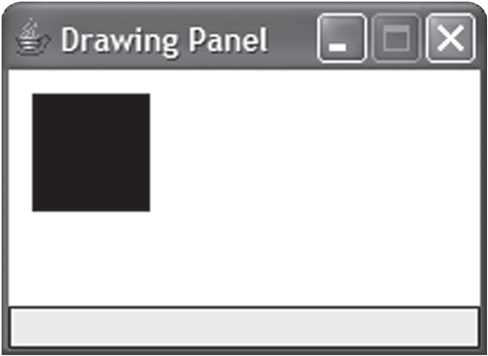
\includegraphics[width=\maxwidth,height=\maxheight,width=0.9\linewidth]{Figures/img_p190_1.png}
\end{center}

\textbf{4.} Đoạn mã sau cố gắng vẽ một hình chữ nhật màu đen từ
\texttt{(10,\ 20)} đến \texttt{(50,\ 40)} với một đường cắt ngang đường
chéo của nó:

\begin{verbatim}
DrawingPanel panel = new DrawingPanel(200, 100);
Graphics g = panel.getGraphics();
g.drawRect(10, 20, 50, 40);
g.drawLine(10, 20, 50, 40);
\end{verbatim}

Tuy nhiên, đầu ra đồ họa lại trông giống như Hình 3G.20 thay thế. Phải
thay đổi điều gì để nó trông như dự định?

Hình 3G.20 Đầu ra đồ họa của Bài tự kiểm tra (Self-Check) 3G.4

\begin{center}
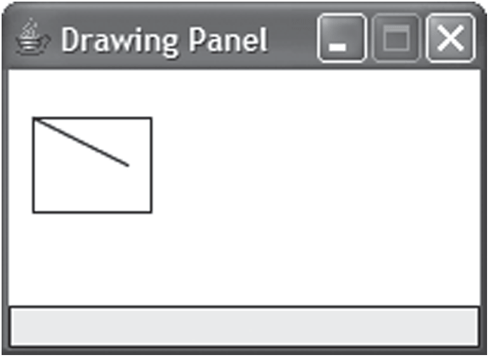
\includegraphics[width=\maxwidth,height=\maxheight,width=0.9\linewidth]{Figures/img_p191_1.png}
\end{center}

\textbf{5.} Loại hình nào sẽ được vẽ bởi chương trình sau? Bạn có thể vẽ
một bức tranh gần giống với hình dạng của nó mà không cần chạy nó trước
không?

\begin{verbatim}
 1  import java.awt.*;
 2
 3  public class Draw7 {
 4      public static void main(String[] args) {
 5          DrawingPanel panel = new DrawingPanel(200, 200);
 6          Graphics g = panel.getGraphics();
 7          for (int i = 0; i < 20; i++) {
 8              g.drawOval(i * 10, i * 10, 200 - (i * 10), 200 - (i * 10));
 9          }
10      }
11  }
\end{verbatim}

\subsection{Bài tập (Exercises)}\label{buxe0i-tux1eadp-exercises}

\textbf{1.} Viết một chương trình sử dụng \texttt{DrawingPanel} để vẽ
Hình 3G.21.

Hình 3G.21 Đầu ra đồ họa mong muốn của Bài tập 3G.1

\begin{center}

\includegraphics[width=\maxwidth,height=\maxheight,width=0.9\linewidth]{Figures/img_p193_1.png}
\end{center}

Cửa sổ rộng 220 pixel và cao 150 pixel. Hình nền màu vàng. Có hai hình
bầu dục màu xanh dương có kích thước \(40 \times 40\) pixel. Chúng cách
nhau 80 pixel, và góc trên bên trái của hình bầu dục bên trái nằm ở vị
trí \texttt{(50,\ 25)}. Có một hình vuông màu đỏ mà hai góc trên của nó
cắt chính xác tâm của hai hình bầu dục. Cuối cùng, có một đường ngang
màu đen đi qua tâm của hình vuông.

\textbf{2.} Sửa đổi chương trình của bạn từ bài tập trước để vẽ hình
bằng một phương thức có tên là \texttt{drawFigure}. Phương thức nên chấp
nhận ba tham số: \texttt{Graphics\ g} của \texttt{DrawingPanel} để vẽ
lên, và một cặp tọa độ \((x, y)\) chỉ định vị trí của góc trên bên trái
của hình. Sử dụng tiêu đề (heading) sau cho phương thức của bạn:

\begin{verbatim}
public static void drawFigure(Graphics g, int x, int y)
\end{verbatim}

Đặt kích thước của \texttt{DrawingPanel} của bạn thành
\(450 \times 150\) pixel và sử dụng phương thức \texttt{drawFigure} của
bạn để đặt hai hình lên đó, như được hiển thị trong Hình 3G.22. Một hình
nên ở vị trí \texttt{(50,\ 25)} và hình kia nên ở vị trí
\texttt{(250,\ 45)}.

Hình 3G.22 Đầu ra đồ họa mong muốn của Bài tập 3G.2

\begin{center}

\includegraphics[width=\maxwidth,height=\maxheight,width=0.9\linewidth]{Figures/img_p194_0.png}
\end{center}

\textbf{3.} Giả sử bạn có chương trình hiện tại sau đây tên là
\texttt{Face}, sử dụng \texttt{DrawingPanel} để vẽ hình khuôn mặt được
hiển thị trong Hình 3G.23. Sửa đổi chương trình để vẽ đầu ra đã được sửa
đổi hiển thị trong Hình 3G.24. Hãy làm như vậy bằng cách viết một phương
thức được tham số hóa (parameterized method) để vẽ một khuôn mặt ở các
vị trí khác nhau. Kích thước cửa sổ nên được thay đổi thành
\(320 \times 180\) pixel, và góc trên bên trái của hai khuôn mặt nằm ở
\texttt{(10,\ 30)} và \texttt{(150,\ 50)}.

Hình 3G.23 Đầu ra đồ họa ban đầu của Bài tập 3G.3

\begin{center}

\includegraphics[width=\maxwidth,height=\maxheight,width=0.9\linewidth]{Figures/img_p195_1.png}
\end{center}

Hình 3G.24 Đầu ra đồ họa mong muốn của Bài tập 3G.3

\begin{center}

\includegraphics[width=\maxwidth,height=\maxheight,width=0.9\linewidth]{Figures/img_p196_1.png}
\end{center}

\begin{verbatim}
 1  public class Face {
 2      public static void main(String[] args) {
 3          DrawingPanel panel = new DrawingPanel(220, 150);
 4          Graphics g = panel.getGraphics();
 5
 6          g.setColor(Color.BLACK);
 7          g.drawOval(10, 30, 100, 100);   // face outline
 8
 9          g.setColor(Color.BLUE);
10          g.fillOval(30, 60, 20, 20);     // eyes
11          g.fillOval(70, 60, 20, 20);
12
13          g.setColor(Color.RED);          // mouth
14          g.drawLine(40, 100, 80, 100);
15      }
16  }
\end{verbatim}

\textbf{4.} Sửa đổi chương trình \texttt{Face} trước đó của bạn để vẽ
đầu ra mới được hiển thị trong Hình 3G.25. Kích thước cửa sổ nên được
thay đổi thành \(520 \times 180\) pixel, và các góc trên bên trái của
các khuôn mặt nằm ở \texttt{(10,\ 30)}, \texttt{(110,\ 30)},
\texttt{(210,\ 30)}, \texttt{(310,\ 30)} và \texttt{(410,\ 30)}.

Hình 3G.25 Đầu ra đồ họa mong muốn của Bài tập 3G.4

\begin{center}

\includegraphics[width=\maxwidth,height=\maxheight,width=0.9\linewidth]{Figures/img_p198_1.png}
\end{center}

\textbf{5.} Viết một chương trình tên là \texttt{ShowDesign} sử dụng
\texttt{DrawingPanel} để vẽ Hình 3G.26.

Hình 3G.26 Đầu ra đồ họa mong muốn của Bài tập 3G.5

\begin{center}
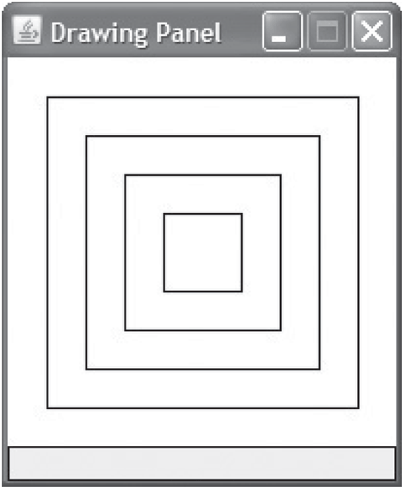
\includegraphics[width=\maxwidth,height=\maxheight,width=0.9\linewidth]{Figures/img_p199_0.png}
\end{center}

Cửa sổ rộng 200 pixel và cao 200 pixel. Màu nền là màu trắng và màu tiền
cảnh là màu đen. Khoảng cách giữa bốn hình chữ nhật là 20 pixel, và các
hình chữ nhật là đồng tâm (tâm của chúng nằm ở cùng một điểm). Sử dụng
vòng lặp để vẽ các hình chữ nhật lặp đi lặp lại.

\textbf{6.} Sửa đổi chương trình \texttt{ShowDesign} của bạn từ bài tập
trước sao cho nó có một phương thức chấp nhận các tham số về chiều rộng
và chiều cao của cửa sổ, và hiển thị các hình chữ nhật ở kích thước phù
hợp. Ví dụ: nếu phương thức của bạn được gọi với các giá trị
\texttt{300} và \texttt{100}, cửa sổ sẽ trông giống như Hình 3G.27.

Hình 3G.27 Đầu ra đồ họa mong muốn của Bài tập 3G.6

\begin{center}
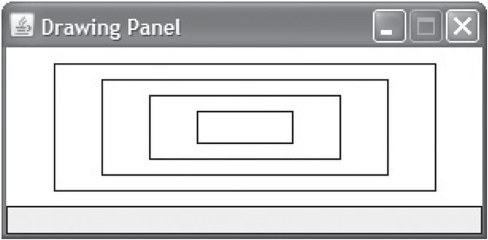
\includegraphics[width=\maxwidth,height=\maxheight,width=0.9\linewidth]{Figures/img_p200_0.png}
\end{center}

\textbf{7.} Viết một chương trình tên là \texttt{Squares} sử dụng
\texttt{DrawingPanel} để vẽ hình dạng hiển thị trong Hình 3G.28.

Hình 3G.28 Đầu ra đồ họa mong muốn của Bài tập 3G.7

\begin{center}

\includegraphics[width=\maxwidth,height=\maxheight,width=0.9\linewidth]{Figures/img_p200_1.png}
\end{center}

\texttt{DrawingPanel} có kích thước rộng 300 pixel và cao 200 pixel.
Hình nền của nó là màu lục lam (cyan). Các đường ngang và dọc được vẽ
bằng màu đỏ và đường chéo được vẽ bằng màu đen. Góc trên bên trái của
đường chéo nằm ở \texttt{(50,\ 50)}. Các đường ngang và dọc liên tiếp
cách nhau 20 pixel.

\textbf{8.} Sửa đổi mã của bạn từ bài tập trước để tạo ra hoa văn được
hiển thị trong Hình 3G.29.

Hình 3G.29 Đầu ra đồ họa mong muốn của Bài tập 3G.8

\begin{center}

\includegraphics[width=\maxwidth,height=\maxheight,width=0.9\linewidth]{Figures/img_p201_1.png}
\end{center}

\texttt{DrawingPanel} bây giờ có kích thước \(400 \times 300\) pixel.
Hình đầu tiên nằm ở vị trí cũ, \texttt{(50,\ 50)}. Các hình khác lần
lượt ở vị trí \texttt{(250,\ 10)} và \texttt{(180,\ 115)}. Sử dụng một
hoặc nhiều phương thức tĩnh có tham số (parameterized static methods) để
giảm sự lặp lại trong giải pháp của bạn.

\textbf{9.} Sửa đổi mã của bạn từ bài tập trước để tạo ra hoa văn được
hiển thị trong Hình 3G.30.

Hình 3G.30 Đầu ra đồ họa mong muốn của Bài tập 3G.9

\begin{center}

\includegraphics[width=\maxwidth,height=\maxheight,width=0.9\linewidth]{Figures/img_p202_1.png}
\end{center}

\texttt{DrawingPanel} giống như bài trước ngoại trừ việc bây giờ mỗi
hình có một kích thước khác nhau. Hình bên trái có kích thước ban đầu là
100, hình trên cùng bên phải có kích thước là 50, và hình dưới cùng bên
phải có kích thước là 180. Sử dụng các phương thức tĩnh có tham số
(parameterized static methods) để giảm sự dư thừa của giải pháp của bạn.

\textbf{10.} Viết một chương trình tên là \texttt{Stairs} sử dụng
\texttt{DrawingPanel} để vẽ hình hiển thị trong Hình 3G.31. Góc trên bên
trái của bậc thang đầu tiên nằm ở vị trí \texttt{(5,\ 5)}. Bậc thang đầu
tiên có kích thước \(10 \times 10\) pixel. Mỗi bậc thang rộng hơn bậc
trên nó 10 pixel. Tạo một bảng gồm các tọa độ \((x, y)\) và kích thước
\((\text{width} \times \text{height})\) của năm bậc thang đầu tiên. Lưu
ý những giá trị nào thay đổi và những giá trị nào không đổi.

Hình 3G.31 Đầu ra đồ họa mong muốn của Bài tập 3G.10

\begin{center}
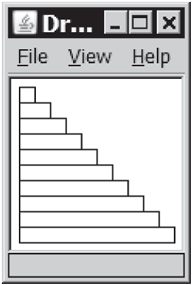
\includegraphics[width=\maxwidth,height=\maxheight,width=0.9\linewidth]{Figures/img_p204_0.png}
\end{center}

\textbf{11.} Sửa đổi chương trình \texttt{Stairs} trước đó của bạn để vẽ
từng đầu ra được hiển thị trong Hình 3G.32. Chỉ sửa đổi phần thân của
vòng lặp của bạn. (Bạn có thể muốn tạo một bảng mới để tìm biểu thức cho
\(x\), \(y\), chiều rộng và chiều cao cho từng đầu ra mới.)

Hình 3G.32 Đầu ra đồ họa mong muốn của Bài tập 3G.11

\begin{center}

\includegraphics[width=\maxwidth,height=\maxheight,width=0.9\linewidth]{Figures/img_p204_1.png}
\end{center}

\textbf{12.} Viết một chương trình tên là \texttt{Triangle} sử dụng
\texttt{DrawingPanel} để vẽ hình hiển thị trong Hình 3G.33.

Hình 3G.33 Đầu ra đồ họa mong muốn của Bài tập 3G.12

\begin{center}

\includegraphics[width=\maxwidth,height=\maxheight,width=0.9\linewidth]{Figures/img_p205_2.png}
\end{center}

Cửa sổ có kích thước \(600 \times 200\) pixel. Nền màu vàng và các đường
vẽ màu xanh dương. Các đường vẽ cách nhau 10 pixel theo chiều dọc và các
đường chéo giao nhau ở dưới cùng của hình, tại chính giữa theo chiều
ngang.

\textbf{13.} Viết một chương trình tên là \texttt{Football} sử dụng
\texttt{DrawingPanel} để vẽ hình hiển thị trong Hình 3G.34. Mặc dù hình
trông có vẻ chứa các đường cong, nhưng nó hoàn toàn được tạo thành từ
các đường thẳng.

Hình 3G.34 Đầu ra đồ họa mong muốn của Bài tập 3G.13

\begin{center}

\includegraphics[width=\maxwidth,height=\maxheight,width=0.9\linewidth]{Figures/img_p206_1.png}
\end{center}

Cửa sổ có kích thước \(250 \times 250\) pixel. Có một hình chữ nhật bên
ngoài từ \texttt{(10,\ 30)} đến \texttt{(210,\ 230)} và một tập hợp các
đường màu đen được vẽ xung quanh các cạnh cách nhau mỗi 10 pixel. Ví dụ:
dọc theo phía trên bên trái có một đường từ \texttt{(10,\ 200)} đến
\texttt{(20,\ 30)}, một đường từ \texttt{(10,\ 190)} đến
\texttt{(30,\ 30)}, một đường từ \texttt{(10,\ 180)} đến
\texttt{(40,\ 30)},\ldots{} và dọc theo phía dưới bên phải có một đường
từ \texttt{(20,\ 210)} đến \texttt{(210,\ 200)}, một đường từ
\texttt{(30,\ 210)} đến \texttt{(210,\ 190)}, v.v.

\subsection{Dự án Lập trình (Programming
Projects)}\label{dux1ef1-uxe1n-lux1eadp-truxecnh-programming-projects-1}

\textbf{1.} Viết một chương trình vẽ các hoa văn hiển thị trong Hình
3G.35 lên một \texttt{DrawingPanel}.

Hình 3G.35 Đầu ra đồ họa mong muốn của Dự án Lập trình 3G.1

\begin{center}

\includegraphics[width=\maxwidth,height=\maxheight,width=0.9\linewidth]{Figures/img_p208_1.png}
\end{center}

Kích thước của \texttt{DrawingPanel} là \(400 \times 400\) pixel và màu
nền của nó là màu lục lam (cyan). Nó chứa bốn hình bao gồm các hình tròn
đồng tâm màu vàng với viền đen, tất cả được bao quanh bởi một hình chữ
nhật màu xanh lá cây có viền đen. Bốn hình trên \texttt{DrawingPanel}
của bạn phải có các thuộc tính được hiển thị trong Bảng 3G.7.

Bảng 3G.7 Các thuộc tính của hình tròn

Chia nhỏ chương trình của bạn thành các phương thức để vẽ một hình con
cũng như các lưới hình con lớn hơn, chẳng hạn như lưới \(5 \times 5\) ở
vị trí \texttt{(10,\ 120)}.

\textbf{2.} Viết một chương trình vẽ hình ảnh được hiển thị trong Hình
3G.36 lên một \texttt{DrawingPanel} có kích thước \(200 \times 200\).
Mỗi con tem (stamp) có kích thước \(50 \times 50\) pixel.

Hình 3G.36 Đầu ra đồ họa mong muốn của Dự án Lập trình 3G.2

\begin{center}

\includegraphics[width=\maxwidth,height=\maxheight,width=0.9\linewidth]{Figures/img_p209_0.png}
\end{center}

\textbf{3.} Viết một chương trình vẽ các bàn cờ (checkerboards) giống
như được hiển thị trong Hình 3G.37 lên một \texttt{DrawingPanel} có kích
thước \(420 \times 300\).

Hình 3G.37 Đầu ra đồ họa mong muốn của Dự án Lập trình 3G.3

\begin{center}

\includegraphics[width=\maxwidth,height=\maxheight,width=0.9\linewidth]{Figures/img_p210_1.png}
\end{center}

\textbf{4.} Viết một phiên bản sửa đổi của chương trình nghiên cứu điển
hình \texttt{Projectile} từ Chương 3 để vẽ một đồ thị về chuyến bay của
đường đạn (projectile's flight) lên một \texttt{DrawingPanel} có kích
thước \(420 \times 220\). Ví dụ, bảng điều khiển được hiển thị trong
Hình 3G.38 vẽ một đường đạn với vận tốc ban đầu là 30 mét mỗi giây, một
góc là 50 độ, và 10 bước.

Hình 3G.38 Đầu ra đồ họa mong muốn của Dự án Lập trình 3G.4

\begin{center}

\includegraphics[width=\maxwidth,height=\maxheight,width=0.9\linewidth]{Figures/img_p211_1.png}
\end{center}

\textbf{5.} Viết một chương trình vẽ hình ảnh được hiển thị trong Hình
3G.39 lên một \texttt{DrawingPanel} có kích thước \(650 \times 400\).
Hình ảnh này đại diện cho một ảo ảnh quang học nổi tiếng được gọi là
``Cafe Wall'', trong đó một loạt các hình vuông thẳng (straight squares)
dường như bị nghiêng.

Hình 3G.39 Đầu ra đồ họa mong muốn của Dự án Lập trình 3G.5

\begin{center}

\includegraphics[width=\maxwidth,height=\maxheight,width=0.9\linewidth]{Figures/img_p212_1.png}
\end{center}

Hình ảnh có nền màu xám và nhiều hàng hình vuông màu đen và màu trắng
với một chữ X màu xanh dương được vẽ xuyên qua mỗi hình vuông màu đen.
Hai hàng đứng tự do (free-standing rows) trong sơ đồ có các thuộc tính
sau:

Bảng 3G.8 Các thuộc tính của hàng Cafe Wall

\begin{center}
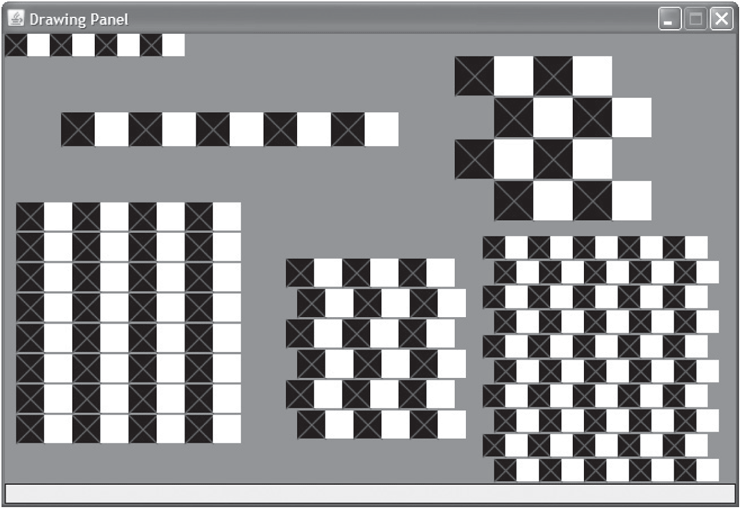
\includegraphics[width=\maxwidth,height=\maxheight,width=0.9\linewidth]{Figures/img_p213_0.png}
\end{center}

Sơ đồ có bốn lưới gồm các hàng hình vuông, với 2 pixel khoảng trống theo
chiều dọc giữa các hàng kề nhau. Một khía cạnh quan trọng của ảo ảnh
quang học là mỗi hàng xen kẽ (every other row) được dịch chuyển theo
chiều ngang bởi một phần bù (offset) cụ thể. Bốn lưới có các thuộc tính
sau:

Bảng 3G.9 Các thuộc tính của lưới Cafe Wall
